% Édition française OpenLogic : 64 unités sur 722, huit chapitres.
% LaTeX cumulatif contenant tout le texte de cette livraison.
% Styles, figures, bibliographie et instructions fournis dans le ZIP source.
\documentclass[11pt,a4paper,openany]{memoir}
\usepackage{mathpazo}
\usepackage{fontspec}
\setmainfont{TeX Gyre Pagella}
\setsansfont{TeX Gyre Heros}
\setmonofont{TeX Gyre Cursor}
\usepackage{natbib}
\newcommand*{\olpath}{../..}
\newcommand*{\ollangid}{fr}
\newcommand*{\ollanguage}{french}
\input{\olpath/sty/open-logic.sty}
\input{\olpath/sty/open-logic-defer.sty}
\includeenv{editorial}
% Les cadres doivent restituer les notes après leur fermeture.
\usepackage{footnotehyper}
\makesavenoteenv{editorial}
\frcompletevariantstrue
% Les renvois hors livraison restent des liens vers leur section originale.
% Dès que la section française est intégrée, son renvoi interne est prioritaire.
\makeatletter
\newcommand{\FRoriginalsection}[2]{%
  section « \href{https://github.com/OpenLogicProject/OpenLogic/blob/9620cc73f9c8e0ad003c514a5d3748f29611c4c0/content/history/set-theory/#1.tex}{#2} »\space
  (dans l'original anglais, hors de cette livraison)}
\csdef{FRexternal@his:set:mythology:sec}{%
  \FRoriginalsection{mythology}{More Myth than History?}}
\csdef{FRexternal@his:set:limits:sec}{%
  \FRoriginalsection{limits}{Rigorous Definition of Limits}}
\csdef{FRexternal@sth:::part}{%
  partie « \href{https://github.com/OpenLogicProject/OpenLogic/blob/9620cc73f9c8e0ad003c514a5d3748f29611c4c0/content/set-theory/set-theory.tex}{Set Theory} »\space
  (dans l'original anglais, hors de cette livraison)}
\csdef{FRexternal@sth:ord-arithmetic::chap}{%
  chapitre « \href{https://github.com/OpenLogicProject/OpenLogic/blob/9620cc73f9c8e0ad003c514a5d3748f29611c4c0/content/set-theory/ord-arithmetic/ord-arithmetic.tex}{Ordinal Arithmetic} »\space
  (dans l'original anglais, hors de cette livraison)}
\RenewDocumentCommand \olref { o o o m } {%
  \begingroup
  \edef\FRrefkey{%
    \IfNoValueTF{#1}
      {\theolpart:\theolchapter:\theolsection}
      {\IfNoValueTF{#2}
        {\theolpart:\theolchapter:#1}
        {\IfNoValueTF{#3}{\theolpart:#1:#2}{#1:#2:#3}}}:#4}%
  \@ifundefined{r@\FRrefkey}
    {\ifcsdef{FRexternal@\FRrefkey}
      {\csuse{FRexternal@\FRrefkey}}{\cref{\FRrefkey}}}
    {\cref{\FRrefkey}}%
  \endgroup}
\makeatother

\problemsperchapter
\setlrmarginsandblock{28mm}{28mm}{*}
\setulmarginsandblock{26mm}{28mm}{*}
\checkandfixthelayout
\linespread{1.05}
\setlength{\emergencystretch}{2em}
\let\cleardoublepage\clearpage
\pagestyle{plain}
\hypersetup{pdftitle={OpenLogic : édition française — Des ensembles à la logique propositionnelle},
pdfauthor={Open Logic Project ; traduction française assistée par IA},
pdfsubject={Ensembles, relations, fonctions, dénombrabilité, nombres et logique propositionnelle},
linkcolor=black,citecolor=black,urlcolor=blue}
\begin{document}
\frontmatter
\begin{titlingpage}
\setlength{\parindent}{0pt}
\vspace*{15mm}
{\sffamily\Huge\bfseries OpenLogic\par}
\vspace{6mm}
{\sffamily\LARGE Édition française\par}
\vspace{14mm}
{\sffamily\huge Des ensembles\\à la logique propositionnelle\par}
\vspace{5mm}
{\large Relations, fonctions, dénombrabilité et nombres :\\
syntaxe, sémantique et systèmes de preuve\par}
\vfill
{\large Sixième livraison : huit chapitres\par}
\vspace{4mm}
Cette livraison comprend cinquante-six sections et leurs huit chapitres d’organisation,
soit 64 des 722 unités de contenu prévues pour l’édition intégrale.
Elle conserve les démonstrations, exemples, figures et exercices
des chapitres originaux. Les précisions éditoriales sont signalées
dans le texte. Les présentations alternatives de la dénombrabilité
sont réunies dans un même chapitre, avec leurs conventions explicites.
Le cinquième chapitre construit les entiers, les rationnels et les réels,
par les coupures de Dedekind et les classes de suites de Cauchy.
Le sixième étudie les ensembles infinis, les algèbres de Dedekind,
la récurrence et une autre preuve du théorème de Schröder--Bernstein.
Le septième présente les formules propositionnelles, leur construction
inductive, les valuations et les notions sémantiques fondamentales.
Le huitième présente les systèmes de preuve, leur correction et leur
complétude : calcul des séquents, déduction naturelle, tableaux et
dérivations axiomatiques.
\vspace{7mm}
\par\small
Texte original : \href{https://openlogicproject.org/}{Open Logic Project}.
Traduction française et révision éditoriale assistées par IA.
Aucune validation humaine indépendante n'est revendiquée.
\par\medskip
Texte original et traduction : licence
\href{https://creativecommons.org/licenses/by/4.0/}{Creative Commons
Attribution 4.0 International}. Les notices de droits propres aux
composants sont conservées avec les sources.
\par\medskip
\href{https://kokunoyumeto.github.io/OpenLogic-translations/}{Catalogue
des traductions d'OpenLogic}
\end{titlingpage}
\tableofcontents*
\mainmatter

% BEGIN embedded source: content/sets-functions-relations/sets/sets.tex
\begingroup
\expandafter\def\csname ol@sectioncs\endcsname{section}
\def\olfilename{sets}


\olchapter{sfr}{set}{Ensembles}


% BEGIN embedded source: content/sets-functions-relations/sets/basics.tex
\begingroup
\expandafter\def\csname ol@sectioncs\endcsname{section}
\def\olfilename{basics}


\olfileid[fr]{sfr}{set}{bas}
\olsection{Extensionnalité}

Un \emph{ensemble} est une collection d'objets considérée comme un seul
objet. Les objets qui le constituent sont appelés ses \emph{éléments}
ou ses \emph{membres}. Si $x$ est !!a{element} d'un ensemble~$A$,
on écrit $x \in A$ ; sinon, on écrit $x \notin A$. L'ensemble qui n'a
aucun !!{element} est appelé l'ensemble \emph{vide} et se note
«~$\emptyset$~».

\begin{explain}
Peu importe la manière dont on \emph{décrit} l'ensemble,
l'\emph{ordre} dans lequel on donne ses !!{element}s, ou même le
\emph{nombre de fois} où on les énumère. Seule compte l'identité
de ses !!{element}s. Le principe suivant exprime cette idée.
\end{explain}

\begin{defn}[Extensionnalité]
  Si $A$ et $B$ sont des ensembles, alors $A = B$ si et seulement si
  tout !!{element} de~$A$ est aussi !!a{element} de~$B$, et
  réciproquement.
\end{defn}

L'extensionnalité justifie certaines notations. En général, étant donnés
des objets $a_{1}$, \dots, $a_{n}$, on note $\{a_{1}, \dots, a_{n}\}$
\emph{l'}ensemble dont les !!{element}s sont $a_1, \ldots, a_n$.
L'article défini est essentiel : l'extensionnalité nous dit qu'il ne
peut y avoir qu'\emph{un seul} ensemble de ce type. Elle justifie
également l'égalité suivante :
  \[
    \{a, a, b\} = \{a, b\} = \{b,a\}.
  \]
On retrouve ainsi l'idée que, pour les ensembles, ni l'ordre dans
lequel on indique les !!{element}s ni le nombre de leurs occurrences
n'importent.

\begin{tagblock}{novice}
\begin{ex}
Lorsqu'on dispose d'objets, on peut les réunir en un ensemble.
Par exemple, l'ensemble des frères et sœurs de Richard contient
une personne et peut s'écrire $S=\{\textrm{Ruth}\}$.
L'ensemble des entiers strictement positifs inférieurs à $4$ est
$\{1, 2, 3\}$ ; on peut aussi l'écrire $\{3, 2, 1\}$ ou même
$\{1, 2, 1, 2, 3\}$. Il s'agit chaque fois du même ensemble,
par extensionnalité : tout !!{element} de $\{1, 2, 3\}$ est aussi
!!a{element} de $\{3, 2, 1\}$ (et de $\{1, 2, 1, 2, 3\}$), et
réciproquement.
\end{ex}
\end{tagblock}

Nous décrirons souvent un ensemble à l'aide d'une propriété commune
à ses !!{element}s. Nous utiliserons pour cela la notation abrégée
$\Setabs{x}{\phi(x)}$, où $\phi(x)$ désigne la propriété que~$x$
doit vérifier pour figurer parmi les !!{element}s de l'ensemble.

\begin{tagblock}{novice}
\begin{ex}
Dans notre exemple, nous aurions aussi pu définir $S$ par
\[
S = \Setabs{x}{x \text{ est un frère ou une sœur de Richard}}.
\]
\end{ex}
\end{tagblock}

\begin{tagblock}{math}
\begin{ex}
Un entier strictement positif est dit \emph{parfait} si et seulement
s'il est égal à la somme de ses diviseurs propres positifs
(c'est-à-dire des entiers positifs qui le divisent et lui sont
strictement inférieurs).\footnote{Précision de l'édition française :
les diviseurs considérés sont positifs, et la notion de nombre parfait
porte ici sur les entiers strictement positifs.}
Par exemple, $6$ est parfait, car ses diviseurs propres positifs
sont $1$, $2$ et~$3$, et $6 = 1 + 2 + 3$. En fait, $6$ est le seul
entier strictement positif inférieur à $10$ qui soit parfait.
L'extensionnalité nous permet donc d'écrire :
\[
	\{6\} = \Setabs{x}{x\text{ est parfait et }0 \leq x \leq 10}
\]
La notation de droite se lit «~l'ensemble des $x$ tels que $x$
est parfait et $0 \leq x \leq 10$~». Cette égalité confirme que
la manière de décrire un ensemble n'importe pas. Plus généralement,
l'extensionnalité garantit qu'il y a au plus un ensemble des $x$
tels que $\phi(x)$. Elle justifie donc que l'on appelle
$\Setabs{x}{\phi(x)}$ \emph{l'}ensemble des $x$ tels que~$\phi(x)$,
s'il existe.\footnote{La condition d'existence est explicitée ici ;
la section consacrée au paradoxe de Russell en explique la nécessité.}
\end{ex}
\end{tagblock}

L'extensionnalité fournit une méthode pour montrer que deux ensembles
sont égaux : pour établir $A = B$, on montre que, si $x \in A$,
alors $x \in B$, et que, si $y \in B$, alors $y \in A$.

\begin{prob}
Démontrer qu'il existe au plus un ensemble vide : si $A$ et $B$ sont
des ensembles sans !!{element}, montrer que $A = B$.
\end{prob}


\endgroup
% END embedded source: content/sets-functions-relations/sets/basics.tex



% BEGIN embedded source: content/sets-functions-relations/sets/subsets.tex
\begingroup
\expandafter\def\csname ol@sectioncs\endcsname{section}
\def\olfilename{subsets}


\olfileid[fr]{sfr}{set}{sub}
\olsection{Sous-ensembles et ensembles des parties}

\begin{explain}
Nous voudrons souvent comparer des ensembles. Une comparaison
naturelle consiste à vérifier si \emph{tout ce qui appartient à
l'un appartient aussi à l'autre}. Cette situation est assez
importante pour justifier une nouvelle notation.
\end{explain}

\begin{defn}[Sous-ensemble]
Si tout !!{element} d'un ensemble $A$ est aussi !!a{element} de~$B$,
on dit que $A$ est un \emph{sous-ensemble}, ou une \emph{partie},
de~$B$, et on écrit $A \subseteq B$. Si $A$ n'est pas un
sous-ensemble de~$B$, on écrit $A \not\subseteq B$.
Si $A \subseteq B$ mais $A \neq B$, on écrit $A \subsetneq B$
et on dit que $A$ est un \emph{sous-ensemble strict} de $B$.
\end{defn}

\begin{ex}
Tout ensemble est un sous-ensemble de lui-même, et $\emptyset$ est
un sous-ensemble de tout ensemble. L'ensemble des entiers naturels
pairs est un sous-ensemble de l'ensemble des entiers naturels.
On a aussi $\{ a, b \} \subseteq \{ a, b, c \}$. En revanche,
si $e$ est distinct de $a$, $b$ et $c$, l'ensemble $\{ a, b, e \}$
n'est pas un sous-ensemble de $\{ a, b, c \}$.\footnote{L'hypothèse
sur $e$, implicite dans l'exemple original, est rendue explicite.}
\end{ex}

\begin{ex}
Le nombre $2$ est un !!{element} de l'ensemble des entiers relatifs,
tandis que l'ensemble des entiers pairs en est un sous-ensemble.
Un ensemble peut toutefois être \emph{à la fois} un !!{element}
et un sous-ensemble d'un autre ensemble : par exemple,
$\{0\} \in \{0, \{0\}\}$ et $\{0\} \subseteq \{0, \{0\}\}$.
\end{ex}

L'extensionnalité donne un critère d'égalité des ensembles :
$A = B$ si et seulement si tout !!{element} de~$A$ est aussi
!!a{element} de~$B$, et réciproquement. La définition de
«~sous-ensemble~» donne à $A \subseteq B$ exactement le sens de
la première moitié de ce critère : tout !!{element} de~$A$ est
aussi !!a{element} de~$B$. Elle s'applique également en échangeant
$A$ et $B$ : $B \subseteq A$ si et seulement si tout !!{element}
de~$B$ est aussi !!a{element} de~$A$. C'est précisément ce
qu'exprime «~et réciproquement~» dans le principe d'extensionnalité.
Autrement dit, ce principe entraîne que deux ensembles sont égaux
si et seulement si chacun est un sous-ensemble de l'autre.

\begin{prop}
$A = B$ si et seulement si $A \subseteq B$ et $B \subseteq A$.
\end{prop}

Introduisons à présent quelques notations utiles. Pour définir
l'inclusion de $A$ dans~$B$, nous avons utilisé l'expression
«~tout !!{element} de~$A$ est \dots~», en remplaçant «~$\dots$~»
par «~!!a{element} de $B$~». Cette \emph{forme}
d'expression est si fréquente qu'une notation formelle nous
sera utile.

\begin{defn}\ollabel{forallxina}
$(\forall x \in A)\phi$ abrège $\forall x(x \in A \lif
\phi)$. De même, $(\exists x \in A)\phi$ abrège $\exists x(x
\in A \land \phi)$.
\end{defn}

Avec cette notation, $A \subseteq B$ si et seulement si
$(\forall x \in A)x \in B$.

Considérons maintenant un type particulier d'ensemble :
l'ensemble de tous les sous-ensembles d'un ensemble donné.

\begin{defn}[Ensemble des parties]
L'ensemble de tous les sous-ensembles d'un ensemble~$A$ est appelé
l'\emph{ensemble des parties de}~$A$ et se note $\Pow{A}$.
  \[
    \Pow{A} = \Setabs{B}{B \subseteq A}
  \]
\end{defn}

\begin{ex}
Quels sont tous les sous-ensembles possibles de $\{ a, b, c \}$ ?
Ce sont $\emptyset$, $\{a \}$, $\{b\}$, $\{c\}$, $\{a, b\}$,
$\{a, c\}$, $\{b, c\}$ et $\{a, b, c\}$. L'ensemble de tous
ces sous-ensembles est $\Pow{\{a,b,c\}}$ :
\[
\Pow{\{ a, b, c \}} = \{\emptyset, \{a \}, \{b\}, \{c\}, \{a, b\},
\{b, c\}, \{a, c\}, \{a, b, c\}\}
\]
\end{ex}

\begin{prob}
Énumérer tous les sous-ensembles de $\{a, b, c, d\}$.
\end{prob}

\begin{prob}
Montrer que, si $A$ a $n$ !!{element}s, alors $\Pow{A}$ a
$2^n$ !!{element}s.
\end{prob}


\endgroup
% END embedded source: content/sets-functions-relations/sets/subsets.tex



% BEGIN embedded source: content/sets-functions-relations/sets/important-sets.tex
\begingroup
\expandafter\def\csname ol@sectioncs\endcsname{section}
\def\olfilename{important-sets}


\olfileid[fr]{sfr}{set}{imp}
\olsection{Quelques ensembles importants}

\begin{ex}
Nous étudierons surtout des ensembles dont les !!{element}s sont
des objets mathématiques. Quatre d'entre eux sont assez importants
pour porter un nom particulier :
\begin{multline*}
    \Nat = \{0, 1, 2, 3, \ldots\} \\
    \shoveright{\text{l'ensemble des entiers naturels}}\\
    \shoveleft{\Int = \{\ldots, -2, -1, 0, 1, 2, \ldots\}} \\
    \shoveright{\text{l'ensemble des entiers relatifs}}\\
    \shoveleft{\Rat = \Setabs{\nicefrac{m}{n}}{m, n \in \Int\text{ et }n \neq 0}}\\
    \shoveright{\text{l'ensemble des nombres rationnels}}\\
    \shoveleft{\Real = (-\infty, \infty)}\\
    \text{l'ensemble des nombres réels (le continu)}
\end{multline*}
Ce sont tous des ensembles \emph{infinis} : chacun possède une
infinité d'!!{element}s.

En passant d'un ensemble au suivant, nous disposons de
\emph{nouveaux} nombres. On voit en effet que
$\Nat \subseteq \Int \subseteq \Rat \subseteq \Real$ :
tout entier naturel est un entier relatif ; tout entier relatif
est rationnel ; tout nombre rationnel est réel.
On voit également que $\Nat \subsetneq \Int \subsetneq \Rat$,
puisque $-1$ est un entier relatif qui n'est pas naturel, et
$\nicefrac{1}{2}$ est rationnel sans être entier.
Il est moins évident que $\Rat \subsetneq \Real$, c'est-à-dire
qu'il existe des nombres réels non rationnels\oliflabeldef{sfr:arith:real:realline}{,
mais nous y reviendrons plus loin (\olref[arith][real]{realline})}{}.

Nous utiliserons aussi parfois l'ensemble des entiers strictement
positifs $\PosInt = \{1, 2, 3, \dots\}$ et l'ensemble formé
des deux premiers entiers naturels, $\Bin = \{0, 1\}$.
\end{ex}

\begin{tagblock}{compsci}
\begin{ex}[Mots]
Un autre exemple intéressant est l'ensemble $A^{*}$ des
\emph{mots finis} sur un alphabet $A$ : toute suite finie
d'éléments de~$A$ est un mot sur $A$. Pour tout alphabet~$A$,
le \emph{mot vide $\Lambda$} fait partie des mots sur~$A$.
Par exemple,
\begin{multline*}
\Bin^*
=\{\Lambda,0,1,00,01,10,11,\\
000,001,010,011,100,101,110,111,0000,\ldots\}.
\end{multline*}
Si $x=x_{1}\ldots x_{n}\in A^{*}$ est un mot formé de $n$
«~lettres~» de $A$, sa \emph{longueur} est~$n$,
et on écrit $\len{x}=n$.
\end{ex}
\end{tagblock}

\begin{ex}[Suites infinies]
Pour tout ensemble $A$, on peut aussi considérer l'ensemble~$A^\omega$
des suites infinies d'!!{element}s de~$A$. Une suite infinie
$a_1a_2a_3a_4\dots$ est une liste d'objets qui se prolonge
indéfiniment dans une seule direction, chacun de ces objets
étant !!a{element} de~$A$.
\end{ex}


\endgroup
% END embedded source: content/sets-functions-relations/sets/important-sets.tex



% BEGIN embedded source: content/sets-functions-relations/sets/unions-and-intersections.tex
\begingroup
\expandafter\def\csname ol@sectioncs\endcsname{section}
\def\olfilename{unions-and-intersections}


\olfileid[fr]{sfr}{set}{uni}
\olsection{Réunions et intersections}

\begin{explain}
Dans la \olref[sfr][set][bas]{sec}, nous avons introduit les définitions
d'ensembles en compréhension, c'est-à-dire de la forme
$\Setabs{x}{\phi(x)}$. On fait ici appel à une propriété~$\phi$,
qui peut mentionner des ensembles déjà définis. Ainsi, si $A$ et~$B$
sont des ensembles, $\Setabs{x}{x \in A \lor x \in B}$ est formé
de tous les objets qui sont des !!{element}s de $A$ ou de~$B$ :
il rassemble les !!{element}s de $A$ et de~$B$.
La \olref{fig:union} représente cette situation : la zone colorée
correspond aux !!{element}s des deux ensembles $A$ et~$B$ réunis.

\begin{figure}
  \olasset{assets/diagrams/union.tikz}
  \caption{La réunion $A \cup B$ de deux ensembles rassemble
    les !!{element}s de $A$ et ceux de~$B$.}
  \ollabel{fig:union}
\end{figure}

Cette opération qui consiste à réunir des ensembles est très
utile et fréquente ; donnons-lui un nom et un symbole.
\end{explain}

\begin{defn}[Réunion]
La \emph{réunion} de deux ensembles $A$ et $B$, notée $A \cup B$,
est l'ensemble de tous les objets qui sont des !!{element}s
de $A$, de $B$, ou des deux.
\[
A \cup B = \Setabs{x}{x \in A \lor x \in B}
\]
\end{defn}

\begin{ex}
Puisque la répétition des !!{element}s n'importe pas, la réunion de
deux ensembles ayant !!a{element} en commun ne contient cet
!!{element} qu'une seule fois. Par exemple,
$\{ a, b, c\} \cup \{ a, 0, 1\} = \{a, b, c, 0, 1\}$.

La réunion d'un ensemble et de l'un de ses sous-ensembles est
simplement le plus grand des deux :
$\{a, b, c \} \cup \{a \} = \{a, b, c\}$.

La réunion d'un ensemble et de l'ensemble vide est égale à
cet ensemble : $\{a, b, c \} \cup \emptyset = \{a, b, c \}$.
\end{ex}

\begin{prob}
Démontrer que, si $A \subseteq B$, alors $A \cup B = B$.
\end{prob}

\begin{explain}
On peut aussi considérer une opération «~duale~» de la réunion :
former l'ensemble de tous les !!{element}s qui appartiennent
à la fois à~$A$ et à~$B$. Cette opération s'appelle
l'\emph{intersection} ; elle est représentée dans
la \olref{fig:intersection}.
\begin{figure}
  \olasset{assets/diagrams/intersection.tikz}
  \caption{L'intersection $A \cap B$ de deux ensembles est
    l'ensemble de leurs !!{element}s communs.}
  \ollabel{fig:intersection}
\end{figure}
\end{explain}

\begin{defn}[Intersection]
L'\emph{intersection} de deux ensembles $A$ et $B$, notée
$A \cap B$, est l'ensemble de tous les objets qui sont
des !!{element}s à la fois de $A$ et de~$B$.
\[
A \cap B = \Setabs{x}{x \in A \land x \in B}
\]
Deux ensembles sont dits \emph{disjoints} si leur intersection
est vide, c'est-à-dire s'ils n'ont aucun !!{element} en commun.
\end{defn}

\begin{ex}
Si deux ensembles n'ont aucun !!{element} en commun, leur
intersection est vide. Dans l'exemple suivant, on suppose que
$a$, $b$ et $c$ sont distincts de $0$ et de $1$ :\footnote{Cette
hypothèse, implicite dans l'exemple original, est rendue explicite.}
$\{ a, b, c\} \cap \{ 0, 1\} = \emptyset$.

S'ils ont des !!{element}s en commun, leur intersection est
l'ensemble de ces !!{element}s. En supposant ici $c\neq d$,
on a $\{a, b, c \} \cap \{a, b, d \} = \{a, b\}$.\footnote{Précision
de l'édition française : l'hypothèse $c\neq d$ suffit pour cet exemple.
Sans elle, un élément commun supplémentaire pourrait apparaître.}

L'intersection d'un ensemble et de l'un de ses sous-ensembles
est simplement le plus petit des deux :
$\{a, b, c\} \cap \{a, b\} = \{a, b\}$.

L'intersection de tout ensemble avec l'ensemble vide est vide :
$\{a, b, c \} \cap \emptyset = \emptyset$.
\end{ex}

\begin{prob}
Démontrer rigoureusement que, si $A \subseteq B$, alors
$A \cap B = A$.
\end{prob}

\begin{explain}
On peut aussi former la réunion ou l'intersection de plus de
deux ensembles. Voici une manière commode de traiter le cas général :
réunissons en un seul ensemble tous les ensembles dont nous voulons
prendre la réunion (ou l'intersection). La réunion des ensembles
de départ est alors l'ensemble des objets qui appartiennent à
au moins un !!{element} de cette famille ; leur intersection
est l'ensemble des objets qui appartiennent à chacun de ses
!!{element}s. Pour l'intersection, nous supposons la famille non vide.
\end{explain}

\begin{defn}
Si $A$ est un ensemble d'ensembles, $\bigcup A$ est l'ensemble
des !!{element}s des !!{element}s de~$A$ :
\begin{align*}
\bigcup A & = \Setabs{x}{x \text{ appartient à un !!{element} de } A},
\text{ soit}\\
& = \Setabs{x}{\text{il existe } B \in A
  \text{ tel que } x \in B}
\end{align*}
\end{defn}

\begin{defn}
Si $A$ est un ensemble non vide d'ensembles, $\bigcap A$ est
l'ensemble des objets communs à tous les éléments de~$A$ :
\begin{align*}
\bigcap A & = \Setabs{x}{x \text{ appartient à tout !!{element} de } A},
\text{ soit}\\
 & = \Setabs{x}{\text{pour tout } B \in A, x \in B}
\end{align*}
\end{defn}
\noindent\emph{Précision de l'édition française.}
L'hypothèse $A\neq\emptyset$ est nécessaire ici : sans elle, la
condition universelle serait vérifiée par tout objet. Si l'on travaille
dans un ensemble ambiant fixé $U$, on peut en revanche définir
l'intersection de la famille vide comme étant $U$.

\begin{ex}
Supposons que $A = \{ \{ a, b \}, \{ a, d, e \}, \{ a, d \} \}$,
avec $b\neq d$.\footnote{Précision de l'édition française :
l'hypothèse $b\neq d$, implicite dans l'exemple original,
garantit que les trois ensembles n'ont aucun élément commun autre que $a$.}
Alors $\bigcup A = \{ a, b, d, e \}$ et $\bigcap A = \{ a \}$.
\end{ex}
\begin{prob}
	Montrer que, si $A$ est un ensemble et $A \in B$,
	alors $A \subseteq \bigcup B$.
\end{prob}

On peut procéder de même pour une suite d'ensembles
$A_1$, $A_2$, \dots
\begin{align*}
\bigcup_i A_i & = \Setabs{x}{x \text{ appartient à l'un des } A_i}\\
\bigcap_i A_i & = \Setabs{x}{x \text{ appartient à chacun des } A_i}.
\end{align*}

Si les ensembles sont \emph{indexés} par un ensemble $I$,
c'est-à-dire si l'on considère un ensemble $A_i$ pour chaque
$i \in I$, on peut aussi employer les abréviations suivantes,
avec $I\neq\emptyset$ pour l'intersection sans ensemble ambiant fixé :
\begin{align*}
	\bigcup_{i \in I} A_i & = \bigcup \Setabs{A_i }{i \in I}\\
	\bigcap_{i \in I} A_i & = \bigcap\Setabs{A_i}{i \in I}
\end{align*}

Enfin, on peut considérer l'ensemble de tous les !!{element}s
de~$A$ qui n'appartiennent pas à~$B$. La \olref{difference}
en donne une représentation.

\begin{figure}
  \olasset{assets/diagrams/difference.tikz}
  \caption{La différence $A \setminus B$ de deux ensembles
    est l'ensemble des !!{element}s de~$A$ qui ne sont pas
    des !!{element}s de~$B$.}
  \ollabel{difference}
\end{figure}

\begin{defn}[Différence]
La \emph{différence ensembliste}~$A \setminus B$ est l'ensemble
de tous les !!{element}s de $A$ qui ne sont pas des !!{element}s
de~$B$, c'est-à-dire
\[
A\setminus B = \Setabs{x}{x\in A \text{ et } x \notin B}.
\]
\end{defn}

\begin{prob}
	Démontrer que, si $A \subsetneq B$,
	alors $B \setminus A \neq \emptyset$.
\end{prob}


\endgroup
% END embedded source: content/sets-functions-relations/sets/unions-and-intersections.tex



% BEGIN embedded source: content/sets-functions-relations/sets/pairs-and-products.tex
\begingroup
\expandafter\def\csname ol@sectioncs\endcsname{section}
\def\olfilename{pairs-and-products}


\olfileid[fr]{sfr}{set}{pai}
\olsection[Couples, n-uplets et produits cartésiens]{Couples, $n$-uplets et produits cartésiens}

\begin{explain}
L'extensionnalité implique que les éléments d'un ensemble ne
sont pas ordonnés. Pour représenter un ordre, nous utilisons
des \emph{couples}, ou \emph{paires ordonnées}, $\tuple{x, y}$.
Dans une paire non ordonnée $\{x, y\}$, l'ordre n'importe pas :
$\{x, y\} = \{y, x\}$. Il importe dans un couple :
si $x \neq y$, alors $\tuple{x, y} \neq \tuple{y, x}$.

Comment représenter les couples en théorie des ensembles ?
Il est essentiel que deux couples soient égaux si et seulement
s'ils ont la même première composante et la même seconde
composante, c'est-à-dire :
\[
  \tuple{a, b}= \tuple{c, d}\text{ si et seulement si }a = c \text{ et }b=d.
\]
La définition de Wiener--Kuratowski permet de définir ainsi
les couples en théorie des ensembles.
\end{explain}

\begin{defn}[Couple]\ollabel{wienerkuratowski}
	$\tuple{a, b} = \{\{a\}, \{a, b\}\}$.
\end{defn}

\begin{prob}
	À l'aide de la \olref[sfr][set][pai]{wienerkuratowski},
	démontrer que $\tuple{a, b}= \tuple{c, d}$ si et seulement si
	$a = c$ et $b=d$.
\end{prob}

\begin{explain}
Une fois les couples définis, nous pouvons les utiliser pour
définir d'autres ensembles. Nous avons parfois besoin de suites
ordonnées de plus de deux objets : des \emph{triplets}
$\tuple{x, y, z}$, des \emph{quadruplets} $\tuple{x, y, z, u}$,
et ainsi de suite. Un triplet peut être représenté par un couple
dont la première composante est elle-même un couple :
$\tuple{x, y, z}$ est $\tuple{\tuple{x, y},z}$.
De même, le quadruplet $\tuple{x,y,z,u}$ est
$\tuple{\tuple{\tuple{x,y},z},u}$, et ainsi de suite.
On parle en général de \emph{$n$-uplets ordonnés}
$\tuple{x_1, \dots, x_n}$.

Certains ensembles de couples, ou plus généralement de
$n$-uplets ordonnés, nous seront utiles.
\end{explain}

\begin{defn}[Produit cartésien]
Étant donnés deux ensembles $A$ et $B$, leur \emph{produit cartésien}
$A \times B$ est défini par
\[
  A \times B = \Setabs{\tuple{x, y}}{x \in A \text{ et } y \in B}.
\]
\end{defn}

\begin{ex}
Si $A = \{0, 1\}$ et $B = \{1, a, b\}$, leur produit est
\[
A \times B = \{ \tuple{0, 1}, \tuple{0, a}, \tuple{0, b},
    \tuple{1, 1}, \tuple{1, a}, \tuple{1, b} \}.
\]
\end{ex}

\begin{ex}
Si $A$ est un ensemble, le produit de $A$ avec lui-même, $A \times A$,
se note aussi~$A^2$. C'est l'ensemble de \emph{tous} les couples
$\tuple{x, y}$ tels que $x, y \in A$.
L'ensemble de tous les triplets $\tuple{x, y, z}$ est $A^3$,
et ainsi de suite. On peut en donner une définition par récurrence :
\begin{align*}
  A^1 & = A\\
  A^{k+1} & = A^k \times A
\end{align*}
\end{ex}

\begin{prob}
Énumérer tous les !!{element}s de $\{1, 2, 3\}^3$.
\end{prob}

\begin{prop}\ollabel{cardnmprod}
Si $A$ a $n$ !!{element}s et $B$ a $m$ !!{element}s, alors
$A \times B$ a $n\cdot m$ éléments.
\end{prop}

\begin{proof}
Pour chaque !!{element}~$x$ de~$A$, il y a $m$ !!{element}s
de la forme $\tuple{x, y} \in A \times B$.
Posons $B_x = \Setabs{\tuple{x, y}}{y \in B}$.
Puisque $x_1 \neq x_2$ entraîne
$\tuple{x_1, y} \neq \tuple{x_2, y}$, on a
$B_{x_1} \cap B_{x_2} = \emptyset$.
Si $A = \{x_1, \dots, x_n\}$, alors
$A \times B = B_{x_1} \cup \dots \cup B_{x_n}$,
qui possède donc $n\cdot m$ !!{element}s.

Pour le visualiser, disposons les !!{element}s de~$A \times B$
dans un tableau :
\[
\begin{array}{rcccc}
  B_{x_1} = & \{\tuple{x_1, y_1} & \tuple{x_1, y_2} & \dots & \tuple{x_1, y_m}\}\\
  B_{x_2} = & \{\tuple{x_2, y_1} & \tuple{x_2, y_2} & \dots & \tuple{x_2, y_m}\}\\
  \vdots & & \vdots\\
  B_{x_n} = & \{\tuple{x_n, y_1} & \tuple{x_n, y_2} & \dots & \tuple{x_n, y_m}\}
\end{array}
\]
Les $x_i$ étant tous distincts, de même que les $y_j$,
les couples de ce tableau sont deux à deux distincts,
et il y en a $n\cdot m$.
\end{proof}

\begin{prob}
Montrer par récurrence sur~$k$ que, pour tout $k \ge 1$,
si $A$ a $n$ !!{element}s, alors $A^k$ a $n^k$ !!{element}s.
\end{prob}

\begin{ex}
Si $A$ est un ensemble, un \emph{mot} sur~$A$ est une suite
finie d'!!{element}s de~$A$. Une telle suite peut être considérée
comme un $n$-uplet d'!!{element}s de~$A$. Par exemple, si
$A = \{a, b, c\}$, la suite «~$bac$~» peut être considérée
comme le triplet~$\tuple{b, a, c}$.
Les mots, c'est-à-dire les suites de symboles, jouent un rôle
essentiel en informatique. Par convention, on considère les
!!{element}s de~$A$ comme des suites de longueur~$1$,
et $\emptyset$ comme la suite de longueur~$0$.
Avec ce codage, l'ensemble des représentations de \emph{tous}
les mots sur~$A$ s'écrit alors\footnote{Précision de l'édition
française : pour un alphabet arbitraire, ce codage peut identifier
des mots de longueurs différentes. Par exemple, si le symbole
$\emptyset$ appartient à $A$, le mot vide et le mot d'une seule
lettre $\emptyset$ ont la même représentation. Pour représenter
les mots sans ambiguïté, on associe en général à chaque
représentation la longueur du mot. La formule de l'original
est conservée ci-dessous comme description des représentations
non munies de leur longueur.}
\[
A^* = \{\emptyset\} \cup A \cup A^2 \cup A^3 \cup \dots
\]
\end{ex}


\endgroup
% END embedded source: content/sets-functions-relations/sets/pairs-and-products.tex



% BEGIN embedded source: content/sets-functions-relations/sets/russells-paradox.tex
\begingroup
\expandafter\def\csname ol@sectioncs\endcsname{section}
\def\olfilename{russells-paradox}


\olfileid[fr]{sfr}{set}{rus}
\olsection{Le paradoxe de Russell}

L'extensionnalité justifie la notation $\Setabs{x}{\phi(x)}$ pour
\emph{l'}ensemble des $x$ tels que~$\phi(x)$. Mais ce qu'elle
justifie \emph{exactement}, c'est ceci : \emph{s'il existe}
un ensemble dont les membres sont tous les objets vérifiant
$\phi$, et eux seuls, \emph{alors} il n'y en a qu'un.
Autrement dit, une fois~$\phi$ fixé, l'ensemble
$\Setabs{x}{\phi(x)}$ est unique, \emph{s'il existe}.

Cette condition est essentielle !{} Toutes les propriétés ne
permettent pas de définir un ensemble par \emph{compréhension} :
certaines ne définissent \emph{aucun} ensemble.
Si toute propriété définissait un ensemble, nous aboutirions
à des contradictions. Le paradoxe de Russell en est l'exemple
le plus célèbre.

Les ensembles peuvent être des !!{element}s d'autres ensembles :
par exemple, l'ensemble des parties d'un ensemble~$A$ est
constitué d'ensembles. Il est donc légitime de se demander
si un ensemble est !!a{element} d'un autre.
Un ensemble peut-il être membre de lui-même ?
Rien dans l'idée intuitive d'ensemble ne semble l'exclure.
Si \emph{tous} les ensembles forment une collection d'objets,
on pourrait penser les rassembler en un seul ensemble :
l'ensemble de tous les ensembles. Étant lui-même un ensemble,
il serait !!a{element} de l'ensemble de tous les ensembles.

Le paradoxe de Russell apparaît lorsqu'on considère la propriété
de ne pas avoir soi-même pour !!{element}, autrement dit
de \emph{ne pas s'appartenir à soi-même}.
Supposons qu'il existe un ensemble de tous les ensembles
qui ne s'appartiennent pas à eux-mêmes. L'ensemble
\[
R = \Setabs{x}{x \notin x}
\]
existe-t-il ? On peut démontrer que non.

\begin{thm}[Paradoxe de Russell]\ollabel{thm:russells-paradox}
	Il n'existe pas d'ensemble $R = \Setabs{x}{x \notin x}$.
\end{thm}

\begin{proof}
Si $R = \Setabs{x}{x \notin x}$ existe, alors
$R \in R$ si et seulement si $R \notin R$,
ce qui est contradictoire.
\end{proof}

\begin{tagblock}{novice}
\begin{explain}
Reprenons cette démonstration plus en détail.
Si $R$ existe, on peut se demander si $R \in R$.
Supposons que $R \in R$. Or $R$ est défini comme
l'ensemble de tous les ensembles qui ne sont pas des
!!{element}s d'eux-mêmes. Si $R \in R$, alors $R$ ne vérifie
pas la propriété qui définit $R$. Mais seuls les ensembles
qui vérifient cette propriété appartiennent à~$R$.
Donc $R$ ne peut pas être !!a{element} de~$R$,
c'est-à-dire $R \notin R$. Mais $R$ ne peut pas à la fois
être et ne pas être !!a{element} de~$R$ :
nous obtenons une contradiction.

Puisque l'hypothèse $R \in R$ conduit à une contradiction,
on a $R \notin R$. Mais cela conduit aussi à une contradiction !{}
En effet, si $R \notin R$, alors $R$ vérifie lui-même
la propriété qui définit $R$. Ainsi, $R$ serait !!a{element} de $R$,
comme tous les autres ensembles qui ne s'appartiennent pas
à eux-mêmes. Là encore, il ne peut pas à la fois
ne pas être et être !!a{element} de~$R$.
\end{explain}
\end{tagblock}

\begin{digress}
Comment construire une théorie des ensembles qui évite
le paradoxe de Russell, c'est-à-dire qui n'affirme pas,
de façon \emph{contradictoire}, l'existence de
$R = \Setabs{x}{x \notin x}$ ?
Il faut poser des axiomes qui précisent exactement
dans quelles conditions les ensembles existent,
et dans quelles conditions ils n'existent pas.

La théorie des ensembles esquissée dans ce chapitre
ne le fait pas : elle est \emph{naïve}.
Elle dit seulement que les ensembles satisfont le principe
d'extensionnalité et qu'à partir d'ensembles donnés, on peut
former leur réunion, leur intersection, etc.
Il est possible de développer la théorie des ensembles
avec davantage de rigueur. \oliflabeldef{cumul:::part}{Ce sera
l'objet de la partie \olref[cumul][][]{part}.
Pour l'instant, nous poursuivrons de manière naïve,
en veillant à éviter les contradictions.}{}
\end{digress}



\endgroup
% END embedded source: content/sets-functions-relations/sets/russells-paradox.tex


\OLEndChapterHook


\endgroup
% END embedded source: content/sets-functions-relations/sets/sets.tex


% BEGIN embedded source: content/sets-functions-relations/relations/relations-complete.tex
\begingroup
\expandafter\def\csname ol@sectioncs\endcsname{section}
\def\olfilename{relations-complete}


\olchapter{sfr}{rel}{Relations}


% BEGIN embedded source: content/sets-functions-relations/relations/relations-as-sets.tex
\begingroup
\expandafter\def\csname ol@sectioncs\endcsname{section}
\def\olfilename{relations-as-sets}


\olfileid[fr]{sfr}{rel}{set}
\olsection{Les relations comme ensembles}

\begin{explain}
Dans la \olref[sfr][set][imp]{sec}, nous avons présenté quelques
ensembles importants : $\Nat$, $\Int$, $\Rat$, $\Real$.
Vous connaissez sans doute déjà certaines relations entre les
!!{element}s de ces ensembles. Chacun porte, par exemple,
une \emph{relation d'ordre} usuelle. Il y a aussi la relation
\emph{être identique à}, que tout objet entretient avec lui-même,
et avec aucun autre objet. Nous rencontrerons bien d'autres
relations intéressantes ; les relations possibles sont encore
plus nombreuses. Avant de les examiner, remarquons que l'on
peut considérer les relations comme des ensembles particuliers.

Rappelons pour cela deux notions de la \olref[sfr][set][pai]{sec}.
Tout d'abord, celle de \emph{couple} : étant donnés $a$ et $b$,
on peut former~$\tuple{a, b}$. Ici, l'ordre des composantes
\emph{importe}. Si $a \neq b$, alors
$\tuple{a, b} \neq \tuple{b, a}$.
La situation diffère de celle des paires non ordonnées,
c'est-à-dire des ensembles à $2$ éléments dans ce cas :
$\{a, b\}=\{b, a\}$.
Ensuite, rappelons le \emph{produit cartésien} : si $A$ et $B$
sont des ensembles, on peut former~$A \times B$, l'ensemble
de tous les couples $\tuple{x, y}$ tels que $x \in A$ et $y \in B$.
En particulier, $A^{2}= A \times A$ est l'ensemble de tous
les couples d'éléments de~$A$.

Considérons maintenant une relation particulière :
la relation $<$ sur l'ensemble~$\Nat$ des entiers naturels.
Formons l'ensemble de tous les couples de nombres $\tuple{n, m}$
tels que $n<m$, c'est-à-dire
\[
  R=\Setabs{\tuple{n, m}}{n, m \in \Nat \text{ et } n<m}.
\]
Il y a un lien étroit entre le fait que $n$ soit strictement
inférieur à $m$ et l'appartenance du couple $\tuple{n, m}$ à $R$ :
\[
      n<m\text{ si et seulement si }\tuple{n, m} \in R.
\]
On peut ainsi, sans perdre d'information, considérer que
l'ensemble $R$ \emph{est} la relation $<$ sur $\Nat$.

De même, on peut construire un sous-ensemble de $\Nat^{2}$
pour toute relation entre entiers naturels.
Réciproquement, à tout ensemble de couples d'entiers naturels
$S \subseteq \Nat^{2}$ correspond une relation :
celle que $n$ entretient avec $m$ si et seulement si
$\tuple{n, m} \in S$. Cela justifie la définition suivante.
\end{explain}

\begin{defn}[Relation binaire]
Une \emph{relation binaire} sur un ensemble $A$ est un
sous-ensemble de~$A^{2}$. Si $R \subseteq A^{2}$ est
une relation binaire sur~$A$ et si $x, y \in A$,
on écrit parfois $Rxy$ (ou $xRy$) pour $\tuple{x, y} \in R$.
\end{defn}

\begin{ex}
  \ollabel{relations}
On peut disposer les couples d'entiers naturels qui
constituent l'ensemble $\Nat^{2}$ dans un tableau à deux dimensions :
\[
  \begin{array}{ccccc}
  \mathbf{\tuple{ 0,0 }} & \tuple{ 0,1 } &
    \tuple{ 0,2 } & \tuple{ 0,3 } & \ldots\\
  \tuple{ 1,0 } & \mathbf{\tuple{ 1,1 }} &
    \tuple{ 1,2 } & \tuple{ 1,3 } & \ldots\\
  \tuple{ 2,0 } & \tuple{ 2,1 } &
    \mathbf{\tuple{ 2,2 }} & \tuple{ 2,3 } & \ldots\\
  \tuple{ 3,0 } & \tuple{ 3,1 } & \tuple{ 3,2 } &
    \mathbf{\tuple{ 3,3 }} & \ldots\\
  \vdots & \vdots & \vdots & \vdots & \mathbf{\ddots}
  \end{array}
\]
La diagonale est indiquée en gras, car le sous-ensemble de $\Nat^2$
formé des couples qui s'y trouvent, c'est-à-dire
\[
  \{\tuple{0,0 }, \tuple{ 1,1 }, \tuple{ 2,2 }, \dots\},
  \]
est la \emph{relation d'identité sur}~$\Nat$.
Cette relation étant fréquente, posons, pour tout ensemble $A$,
$\Id{A}=\Setabs{\tuple{ x,x }}{x \in A}$.
Le sous-ensemble de tous les couples situés au-dessus
de la diagonale, c'est-à-dire
\[
  L = \{\tuple{ 0,1 },\tuple{ 0,2 },\ldots,\tuple{ 1,2 },
  \tuple{ 1,3 }, \dots, \tuple{ 2,3 }, \tuple{ 2,4 },\ldots\},
\]
est la relation \emph{être strictement inférieur à} :
$Lnm$ si et seulement si $n<m$.
Le sous-ensemble des couples situés au-dessous
de la diagonale, c'est-à-dire
\[
  G=\{ \tuple{ 1,0 },\tuple{ 2,0 },\tuple{
    2,1 }, \tuple{ 3,0 },\tuple{ 3,1 },\tuple{ 3,2 }, \dots\},
\]
est la relation \emph{être strictement supérieur à} :
$Gnm$ si et seulement si $n>m$.
Notons ici $I=\Id{\Nat}$.\footnote{Précision de l'édition
française : la notation $I$, utilisée sans définition explicite
dans la suite de l'exemple original, désigne la relation
d'identité sur les entiers naturels.}
La réunion de $L$ et de $I$, que l'on peut noter $K=L\cup I$,
est la relation \emph{être inférieur ou égal à} :
$Knm$ si et seulement si $n \le m$.
De même, $H=G \cup I$ est la relation
\emph{être supérieur ou égal à}.
Ces relations $L$, $G$, $K$ et $H$ sont des relations
particulières appelées des \emph{ordres}.
Les relations $L$ et $G$ ont la propriété qu'aucun entier naturel
n'entretient $L$ ou $G$ avec lui-même : pour tout $n$,
ni $Lnn$ ni $Gnn$.
Les relations qui possèdent cette propriété sont dites
\emph{irréflexives} ; lorsqu'elles sont aussi des ordres,
on les appelle des \emph{ordres stricts}.
\end{ex}

\begin{explain}
Les ordres et l'identité sont des relations importantes
et naturelles. Soulignons cependant que notre définition fait
de \emph{tout} sous-ensemble de $A^{2}$ une relation sur~$A$,
aussi artificielle ou peu naturelle qu'elle puisse paraître.
En particulier, $\emptyset$ est une relation sur tout ensemble :
la \emph{relation vide}, qui ne relie aucun couple d'éléments.
L'ensemble $A^{2}$ lui-même est aussi une relation sur~$A$ :
elle relie tout couple d'éléments et s'appelle la
\emph{relation universelle}. Même un ensemble tel que
$E=\Setabs{\tuple{n, m}}{n>5 \text{ ou } m \times n \ge 34}$
définit une relation, ici entre entiers naturels.
\end{explain}

\begin{prob}
  Énumérer les !!{element}s de la relation $\subseteq$
  sur l'ensemble $\Pow{\{a, b, c\}}$.
\end{prob}


\endgroup
% END embedded source: content/sets-functions-relations/relations/relations-as-sets.tex



% BEGIN embedded source: content/sets-functions-relations/relations/reflections.tex
\begingroup
\expandafter\def\csname ol@sectioncs\endcsname{section}
\def\olfilename{reflections}


\olfileid[fr]{sfr}{rel}{ref}
\olsection{Réflexions philosophiques}

Dans la \olref[set]{sec}, nous avons défini les relations comme
certains ensembles. Arrêtons-nous un instant sur une question
philosophique : que \emph{fait} une telle définition ?
Il est fort douteux que nous voulions dire avoir
\emph{découvert} des identités métaphysiques : par exemple,
que la relation d'ordre sur $\Nat$ \emph{se serait révélée être}
l'ensemble $R= \Setabs{\tuple{n,m}}{n, m \in \Nat\text{ et }
n < m}$ défini dans la \olref[set]{sec}.
Voici trois raisons d'en douter.

Premièrement, dans la \olref[set][pai]{wienerkuratowski},
nous avons défini $\tuple{a, b} = \{\{a\}, \{a, b\}\}$.
Considérons plutôt la définition
$\lVert a, b\rVert = \{\{b\}, \{a, b\}\} = \tuple{b,a}$.
Lorsque $a \neq b$, on a
$\tuple{a, b} \neq \lVert a,b\rVert$.
Pourtant, nous aurions tout aussi bien pu choisir
$\lVert a,b\rVert$ comme définition d'un couple, au lieu de
$\tuple{a,b}$. Les deux définitions auraient aussi bien convenu.
Nous avons donc deux candidats tout aussi satisfaisants
pour «~être~» la relation d'ordre sur les entiers naturels :
\begin{align*}
		R &= \Setabs{\tuple{n,m}}{n, m \in \Nat \text{ et }n < m}\\
		S &= \Setabs{\lVert n,m\rVert}{n, m \in \Nat \text{ et }n < m}.
\end{align*}
Puisque $R \neq S$, par extensionnalité, ils ne peuvent
manifestement pas être \emph{tous deux} identiques à la relation
d'ordre sur~$\Nat$. Mais il serait arbitraire, et donc quelque
peu embarrassant, d'affirmer que c'est $R$, plutôt que $S$
(ou l'inverse), qui \emph{est}, dans les faits, cette relation
d'ordre. Il s'agit d'un exemple très simple d'un argument
contre le réductionnisme ensembliste, rendu célèbre par
Benacerraf en \citeyear{Benacerraf1965}.
Nous y reviendrons à plusieurs reprises.

Deuxièmement, si \emph{toute} relation doit être identifiée
à un ensemble, la relation d'appartenance elle-même, $\in$,
devrait être un ensemble particulier : précisément,
$\Setabs{\tuple{x,y}}{x \in y}$.
Mais cet ensemble existe-t-il ?
Le paradoxe de Russell nous avertit que son existence
ne va pas de soi. En fait,
\oliflabeldef{cumul:::part}{la théorie des ensembles développée
dans la partie \olref[cumul][][]{part} \emph{exclura} l'existence
de cet ensemble.\footnote{En anticipant sur la suite, voici
pourquoi. Supposons, pour raisonner par l'absurde, que
$I = \Setabs{\tuple{x,y}}{x \in y}$ existe.
Alors $\bigcup \bigcup I$ est l'ensemble universel,
ce qui contredit le résultat \olref[sfr][z][sep]{thm:NoUniversalSet}.}}{on peut
développer rigoureusement la théorie des ensembles sous forme
axiomatique, et cette théorie exclura effectivement l'existence
de cet ensemble.}
Ainsi, même si certaines relations peuvent être traitées
comme des ensembles, la relation d'appartenance devra
constituer un cas particulier.

Troisièmement, en «~identifiant~» les relations à des ensembles,
nous nous sommes autorisés à écrire $Rxy$ pour
$\tuple{x,y} \in R$. Cela convient si la relation
d'appartenance, «~$\in$~», est traitée \emph{comme} un prédicat.
Mais si «~$\in$~» désigne un certain type d'ensemble,
l'expression «~$\tuple{x,y} \in R$~» ne consiste plus
qu'en trois termes singuliers désignant des ensembles :
«~$\tuple{x,y}$~», «~$\in$~» et «~$R$~».
Or une telle liste de noms n'est pas plus capable d'exprimer
une proposition que la suite de mots dépourvue de sens :
«~la tasse le pot à crayons la table~».
Là encore, même si certaines relations peuvent être traitées
comme des ensembles, la relation d'appartenance doit constituer
un cas particulier. Cet argument réunit une version simple
du paradoxe frégéen du concept \emph{cheval} et une célèbre
objection que Wittgenstein a adressée à Russell.

Que faut-il en conclure ?
Il n'y a rien de \emph{fautif} à dire que les relations sur
les nombres sont des ensembles, à condition de comprendre
dans quel esprit on le dit. Nous n'affirmons pas une identité
métaphysique. Nous remarquons simplement que, dans certains
contextes, on peut \emph{traiter} certaines relations comme
certains ensembles, et que c'est ce que nous ferons.


\endgroup
% END embedded source: content/sets-functions-relations/relations/reflections.tex



% BEGIN embedded source: content/sets-functions-relations/relations/special-properties.tex
\begingroup
\expandafter\def\csname ol@sectioncs\endcsname{section}
\def\olfilename{special-properties}


\olfileid[fr]{sfr}{rel}{prp}
\olsection{Propriétés particulières des relations}

\begin{intro}
Certains types de relations sont si fréquents qu’on leur a donné des noms
particuliers. Ainsi, $\le$ et~$\subseteq$ mettent les objets de leurs domaines
respectifs (par exemple $\Nat$ pour~$\le$ et $\Pow{A}$ pour~$\subseteq$)
en relation de façons semblables. Pour préciser ce qui rapproche ces
relations et ce qui les distingue, nous les classons selon certaines
propriétés qu’elles peuvent posséder. Certaines combinaisons de ces
propriétés définissent des types de relations particulièrement importants :
les relations d’ordre et les relations d’équivalence.
\end{intro}

\begin{defn}[Réflexivité]
Une relation $R \subseteq A^2$ est \emph{réflexive} si et seulement si,
pour tout $x \in A$, on a $Rxx$.
\end{defn}

\begin{defn}[Transitivité]
Une relation $R \subseteq A^2$ est \emph{transitive} si et seulement si,
chaque fois que $Rxy$ et $Ryz$, on a aussi $Rxz$.
\end{defn}

\begin{defn}[Symétrie]
Une relation~$R \subseteq A^2$ est \emph{symétrique} si et seulement si,
chaque fois que $Rxy$, on a aussi~$Ryx$.
\end{defn}

\begin{defn}[Antisymétrie]
Une relation~$R \subseteq A^2$ est \emph{antisymétrique} si et seulement si,
chaque fois que l’on a à la fois $Rxy$ et $Ryx$, on a $x=y$
(autrement dit : si $x\neq y$, alors $\lnot Rxy$ ou $\lnot Ryx$).
\end{defn}

\begin{explain}
Pour une relation symétrique, $Rxy$ et $Ryx$ sont toujours vraies toutes
les deux ou fausses toutes les deux. Pour une relation antisymétrique,
$Rxy$ et $Ryx$ ne peuvent être vraies toutes les deux que si $x = y$.
Cela n’\emph{exige} pas que $Rxy$ et $Ryx$ soient vraies lorsque $x = y$ ;
cette possibilité n’est simplement pas exclue. Une relation antisymétrique
peut donc être réflexive, mais toute relation antisymétrique n’est pas
nécessairement réflexive. Remarquons aussi qu’être antisymétrique et ne pas
être symétrique sont deux conditions différentes. Une relation peut même
être à la fois symétrique et antisymétrique : c’est le cas, par exemple,
de la relation d’identité.
\end{explain}

\begin{defn}[Connexité]
Une relation $R \subseteq A^2$ est \emph{connexe} si, pour tous $x,y\in A$,
lorsque $x \neq y$, on a $Rxy$ ou~$Ryx$.
\end{defn}

\begin{prob}
Donnez des exemples de relations qui sont (a) réflexives et symétriques
mais non transitives, (b) réflexives et antisymétriques,
(c) antisymétriques et transitives mais non réflexives, et
(d) réflexives, symétriques et transitives. N’utilisez pas de relations
portant sur des nombres ou des ensembles.
\end{prob}

\begin{defn}[Irréflexivité]
Une relation $R \subseteq A^2$ est dite \emph{irréflexive} si,
pour tout $x \in A$, on n’a pas $Rxx$.
\end{defn}

\begin{defn}[Asymétrie]
Une relation $R \subseteq A^2$ est dite \emph{asymétrique} s’il n’existe
aucun couple $x,y\in A$ pour lequel on ait à la fois $Rxy$ et~$Ryx$.
\end{defn}

Si $A \neq \emptyset$, aucune relation irréflexive sur~$A$ n’est réflexive,
et toute relation asymétrique sur~$A$ est aussi antisymétrique.
Il existe cependant, dès que $A$ contient au moins deux éléments,
des relations $R \subseteq A^2$ qui ne sont ni réflexives ni
irréflexives ; et, sur tout ensemble non vide, il existe des relations
antisymétriques qui ne sont pas asymétriques.\footnote{Précision éditoriale :
la première affirmation d’existence de l’original demande au moins deux
éléments. Sur un singleton, les seules relations sont la relation vide,
irréflexive, et la relation d’identité, réflexive.}


\endgroup
% END embedded source: content/sets-functions-relations/relations/special-properties.tex



% BEGIN embedded source: content/sets-functions-relations/relations/equivalence-relations.tex
\begingroup
\expandafter\def\csname ol@sectioncs\endcsname{section}
\def\olfilename{equivalence-relations}


\olfileid[fr]{sfr}{rel}{eqv}

\olsection{Relations d’équivalence}

La relation d’identité sur un ensemble est réflexive, symétrique et
transitive. Les relations~$R$ qui possèdent ces trois propriétés sont
très courantes.

\begin{defn}[Relation d’équivalence]
Une relation $R \subseteq A^2$ réflexive, symétrique et transitive est
appelée une \emph{relation d’équivalence}. Deux !!{element}s $x$ et $y$
de~$A$ sont dits \emph{$R$-équivalents} si~$Rxy$.
\end{defn}

Les relations d’équivalence conduisent à la notion de \emph{classe
d’équivalence}. Une relation d’équivalence découpe son domaine en blocs
qui forment une partition.\footnote{Précision terminologique : l’original
emploie ici « partitions » pour désigner les blocs d’une même partition.}
Dans chaque bloc, tous les objets sont en relation les uns avec les autres ;
aucun objet d’un bloc n’est en relation avec un objet d’un autre bloc.
Il est parfois utile de parler \emph{directement} de ces blocs.
C’est pourquoi nous introduisons la définition suivante.

\begin{defn}\ollabel{def:equivalenceclass}
Soit $R \subseteq A^2$ une relation d’équivalence. Pour chaque $x \in A$,
la \emph{classe d’équivalence} de $x$ dans~$A$ est l’ensemble
$\equivrep{x}{R} = \Setabs{y \in A}{Rxy}$. L’\emph{ensemble quotient}
de $A$ par~$R$ est $\equivclass{A}{R} = \Setabs{\equivrep{x}{R}}{x \in A}$,
c’est-à-dire l’ensemble de ces classes d’équivalence.
\end{defn}

Le résultat suivant justifie cette définition et explique pourquoi les
classes d’équivalence forment bien les blocs d’une partition de~$A$.

\begin{prop}
Si $R \subseteq A^2$ est une relation d’équivalence, alors $Rxy$ si et
seulement si $\equivrep{x}{R} = \equivrep{y}{R}$.
\end{prop}

\begin{proof}
Pour le sens direct, supposons $Rxy$ et soit $z \in \equivrep{x}{R}$.
Par définition, $Rxz$. Comme $R$ est une relation d’équivalence, on a $Ryz$.
Explicitons ce raisonnement : de $Rxy$ et de la symétrie de~$R$, on tire
$Ryx$ ; de $Rxz$ et de la transitivité de~$R$, on tire alors~$Ryz$.
Ainsi, $z \in \equivrep{y}{R}$. Puisque ce raisonnement vaut pour tout
tel objet, $\equivrep{x}{R} \subseteq \equivrep{y}{R}$. De la même manière,
$\equivrep{y}{R} \subseteq \equivrep{x}{R}$. Par extensionnalité,
$\equivrep{x}{R} = \equivrep{y}{R}$.

Pour la réciproque, supposons $\equivrep{x}{R} = \equivrep{y}{R}$.
Comme $R$ est réflexive, $Ryy$, donc $y \in \equivrep{y}{R}$.
L’hypothèse $\equivrep{x}{R} = \equivrep{y}{R}$ donne alors
$y \in \equivrep{x}{R}$. On a donc $Rxy$.
\end{proof}

\begin{ex}
L’arithmétique modulaire fournit un exemple intéressant de relation
d’équivalence. Pour tous $a,b \in \Nat$ et $n \in \PosInt$,\footnote{Précision
éditoriale : on prend ici les deux nombres dans les entiers naturels,
zéro compris, pour que la relation soit définie sur tout le domaine du
quotient ci-dessous. L’original les rangeait avec le module parmi les
entiers strictement positifs.}
on pose $a \equiv_n b$ si et seulement si la division de $a$ par~$n$
donne le même reste que celle de $b$ par~$n$. En symboles : $a \equiv_n b$
si et seulement s’il existe $k \in \Int$ tel que $a - b = kn$.
Pour tout~$n$, $\equiv_n$ est une relation d’équivalence. Elle détermine
exactement $n$ classes d’équivalence distinctes ; autrement dit,
$\equivclass{\Nat}{\equiv_n}$ possède $n$ !!{element}s. Ces classes sont :
l’ensemble des nombres divisibles par $n$ sans reste, soit
$\equivrep{0}{\equiv_n}$ ; l’ensemble des nombres dont la division par $n$
donne le reste~$1$, soit $\equivrep{1}{\equiv_n}$ ; \ldots ; et l’ensemble
des nombres dont la division par~$n$ donne le reste~$n-1$, soit
$\equivrep{n-1}{\equiv_n}$.
\end{ex}

\begin{prob}
Montrez que $\equiv_n$ est une relation d’équivalence pour tout
$n \in \PosInt$, et que $\equivclass{\Nat}{\equiv_n}$ possède exactement
$n$ éléments.
\end{prob}


\endgroup
% END embedded source: content/sets-functions-relations/relations/equivalence-relations.tex



% BEGIN embedded source: content/sets-functions-relations/relations/orders.tex
\begingroup
\expandafter\def\csname ol@sectioncs\endcsname{section}
\def\olfilename{orders}


\olfileid[fr]{sfr}{rel}{ord}
\olsection{Ordres}

\begin{explain}
Dans bien des comparaisons, nous décrivons certains objets comme
« inférieurs », « égaux » ou « supérieurs » à d’autres, sous un certain
rapport. Ces comparaisons font intervenir des relations d’\emph{ordre}.
Il en existe cependant plusieurs types. Certaines exigent que deux objets
quelconques soient comparables, d’autres non. Certaines comprennent
l’identité (comme~$\le$), d’autres l’excluent (comme~$<$).
Il nous sera utile de les classer.
\end{explain}

\begin{defn}[Préordre]
Une relation à la fois réflexive et transitive est appelée un
\emph{préordre}.
\end{defn}

\begin{defn}[Ordre partiel]
Un préordre qui est aussi antisymétrique est appelé un \emph{ordre partiel}.
\end{defn}

\begin{defn}[Ordre linéaire]\ollabel{def:linearorder}
Un ordre partiel qui est aussi connexe est appelé un \emph{ordre total}
ou \emph{ordre linéaire}.
\end{defn}

\begin{ex}
Tout ordre linéaire est aussi un ordre partiel, et tout ordre partiel
est aussi un préordre, mais les réciproques sont fausses.
La relation universelle sur~$A$ est un préordre, car elle est réflexive
et transitive. Mais, si $A$ possède plus d’un !!{element}, cette relation
n’est pas antisymétrique ; ce n’est donc pas un ordre partiel.
\end{ex}

\begin{ex}
Considérons sur~$\Bin^*$ la relation $\preccurlyeq$, qui se lit
\emph{est de longueur inférieure ou égale à} : $x \preccurlyeq y$ si et
seulement si $\len{x} \le \len{y}$. C’est un préordre (réflexif et
transitif), qui est même connexe, mais ce n’est pas un ordre partiel,
car il n’est pas antisymétrique. Ainsi, $01 \preccurlyeq 10$ et
$10 \preccurlyeq 01$, alors que $01 \neq 10$.
\end{ex}

\begin{ex}
La relation $\subseteq$ sur un ensemble d’ensembles est un ordre partiel
important. Ce n’est pas en général un ordre linéaire : si $a \neq b$ et
que l’on considère $\Pow{\{a, b\}} = \{\emptyset, \{a\}, \{b\}, \{a,b\}\}$,
on constate que $\{a\} \nsubseteq \{b\}$, que $\{a\} \neq \{b\}$ et que
$\{b\} \nsubseteq \{a\}$.
\end{ex}

\begin{ex}
La relation de \emph{divisibilité} fournit un ordre partiel qui n’est pas
linéaire. Pour des entiers $n$ et~$m$, on écrit $n \mid m$ pour dire que
$n$ divise $m$ sans reste, c’est-à-dire qu’il existe un entier~$k$ tel que
$m = kn$. Sur~$\Nat$, c’est un ordre partiel, mais pas un ordre linéaire :
par exemple, $2 \nmid 3$ et $3 \nmid 2$. Sur $\Int$, la divisibilité
n’est qu’un préordre, car elle n’est pas antisymétrique : $1 \mid -1$ et
$-1 \mid 1$, alors que $1 \neq -1$.
\end{ex}

\begin{ex}
La relation de \emph{prolongement} sur l’ensemble de suites~$A^*$ se
définit ainsi : $s \sqsubseteq s'$ si et seulement si $s = \emptyseq$
(la suite vide), $s = s'$, ou bien $s = \tuple{s_1, \dots, s_n}$ et
$s' = \tuple{s_1, \dots, s_n, s_{n+1}, \dots, s_m}$.
Lorsque $s \sqsubseteq s'$, on dit aussi que $s$ est un \emph{segment initial}
de~$s'$. La relation de prolongement sur $A^*$ est un ordre partiel.
Elle n’est pas linéaire dès que l’alphabet contient deux symboles distincts :
si $a \neq b$, alors $ab \not\sqsubseteq ba$ et $ba \not\sqsubseteq ab$.
\footnote{Précisions éditoriales : avec au plus un symbole, cet ordre est
linéaire. On considère ici de véritables suites finies, dont la longueur
fait partie de l’identité, conformément à la précision sur le codage des
mots donnée au chapitre précédent.}
\end{ex}

\begin{defn}[Ordre strict]
Un \emph{ordre strict} est une relation irréflexive, asymétrique et transitive.
\end{defn}

\begin{defn}[Ordre linéaire strict]\ollabel{def:strictlinearorder}
Un ordre strict qui est aussi connexe est appelé un \emph{ordre total strict}
ou \emph{ordre linéaire strict}.
\end{defn}

\begin{ex}
$\le$ est l’ordre linéaire correspondant à l’ordre linéaire strict~$<$.
$\subseteq$ est l’ordre partiel correspondant à l’ordre strict~$\subsetneq$.
\end{ex}

On peut transformer tout ordre strict $R$ sur~$A$ en un ordre partiel
en lui ajoutant la diagonale $\Id{A}$, c’est-à-dire tous les
couples~$\tuple{x, x}$. On obtient ainsi la \emph{clôture réflexive} de~$R$.
Réciproquement, on obtient un ordre strict à partir d’un ordre partiel
en en retirant~$\Id{A}$. Les deux résultats suivants le précisent.

\begin{prop}\ollabel{prop:stricttopartial}
Si $R$ est un ordre strict sur~$A$, alors $R^+ = R \cup \Id{A}$ est un
ordre partiel. De plus, si $R$ est un ordre linéaire strict, $R^+$ est
un ordre linéaire.
\end{prop}

\begin{proof}
Supposons que $R$ soit un ordre strict : $R \subseteq A^2$ et $R$ est
irréflexive, asymétrique et transitive. Posons $R^+ = R \cup \Id{A}$.
Il faut montrer que $R^+$ est réflexive, antisymétrique et transitive.

$R^+$ est manifestement réflexive, puisque
$\tuple{x, x} \in \Id{A} \subseteq R^+$ pour tout $x \in A$.

Pour établir l’antisymétrie de $R^+$, supposons, par l’absurde, que
$R^+xy$ et $R^+yx$, mais que $x \neq y$. Puisque
$\tuple{x,y} \in R \cup \Id{A}$ et $\tuple{x, y} \notin \Id{A}$,
on a nécessairement $\tuple{x, y} \in R$, c’est-à-dire $Rxy$.
De même, on a~$Ryx$. Cela contredit l’hypothèse selon laquelle $R$
est asymétrique.

Pour la transitivité, supposons $R^+xy$ et $R^+yz$. Si l’on a à la fois
$\tuple{x, y} \in R$ et $\tuple{y,z} \in R$, alors
$\tuple{x, z} \in R$, puisque $R$ est transitive. Sinon,
$\tuple{x, y} \in \Id{A}$, c’est-à-dire $x = y$, ou bien
$\tuple{y, z} \in \Id{A}$, c’est-à-dire $y = z$.
Dans le premier cas, on a $R^+yz$ par hypothèse et $x = y$, donc $R^+xz$.
Le second cas se traite de la même manière. Dans tous les cas, $R^+xz$ :
$R^+$ est donc aussi transitive.

Pour la dernière affirmation, supposons que $R$ soit en outre connexe.
Pour tous $x \neq y$, on a donc $Rxy$ ou~$Ryx$, c’est-à-dire
$\tuple{x, y} \in R$ ou $\tuple{y, x} \in R$.
Puisque $R \subseteq R^+$, cela reste vrai pour $R^+$, qui est donc
connexe elle aussi.
\end{proof}

\begin{prop}\ollabel{prop:partialtostrict}
Si $R$ est un ordre partiel sur~$A$, alors $R^- = R \setminus \Id{A}$
est un ordre strict. De plus, si $R$ est un ordre linéaire, $R^-$ est
un ordre linéaire strict.
\end{prop}

\begin{proof}
La démonstration est laissée en exercice.
\end{proof}

\begin{prob}
Démontrez la \olref[sfr][rel][ord]{prop:partialtostrict}.
\end{prob}

Le résultat élémentaire suivant établit que les ordres linéaires stricts
possèdent une propriété analogue à l’extensionnalité.

\begin{prop}\ollabel{prop:extensionality-strictlinearorders}
Si $<$ est un ordre linéaire strict sur $A$, alors :
\[
  (\forall a, b \in A)((\forall x \in A)(x < a \liff x < b) \lif a = b).
\]
\end{prop}

\begin{proof}
Supposons $(\forall x \in A)(x < a \liff x < b)$. Si $a < b$, alors
$a < a$, ce qui contredit l’irréflexivité de $<$ ; donc $a \nless b$.
De la même manière, $b \nless a$. Puisque $<$ est connexe, on a $a = b$.
\end{proof}


\endgroup
% END embedded source: content/sets-functions-relations/relations/orders.tex



% BEGIN embedded source: content/sets-functions-relations/relations/graphs.tex
\begingroup
\expandafter\def\csname ol@sectioncs\endcsname{section}
\def\olfilename{graphs}


\olfileid[fr]{sfr}{rel}{grp}
\olsection{Graphes}

Un \emph{graphe} se représente par un diagramme dans lequel des points,
appelés « nœuds » ou « sommets », sont reliés par des arêtes.
Les graphes sont omniprésents en mathématiques discrètes et en informatique.
Ils sont très utiles pour représenter et visualiser des relations et
des structures, qu’il s’agisse d’objets concrets, comme divers réseaux,
ou de structures abstraites, comme les issues possibles d’une décision.
La littérature étudie de nombreux types de graphes : les arêtes peuvent
être orientées ou non, porter ou non des étiquettes ; on peut autoriser
ou interdire une arête reliant un nœud à lui-même, plusieurs arêtes entre
les mêmes nœuds, etc. Les \emph{graphes orientés} entretiennent un lien
particulier avec les relations.

\begin{defn}[Graphe orienté]
Un \emph{graphe orienté} $G = \tuple{V, E}$ est constitué d’un ensemble
de \emph{sommets}~$V$ et d’un ensemble d’\emph{arêtes}~$E \subseteq V^2$.
\end{defn}

\begin{explain}
Selon notre définition, un graphe est simplement un ensemble muni d’une
relation sur cet ensemble. Il est bien sûr naturel d’en attendre une
représentation graphique : on peut le dessiner en traçant une flèche du
sommet~$v_1$ vers le sommet $v_2$ si et seulement si
$\tuple{v_1, v_2} \in E$. La seule différence entre une relation considérée
en elle-même et un graphe est que le graphe précise l’ensemble des sommets ;
il peut donc comporter des sommets isolés. Le point essentiel est que
toute relation~$R$ sur un ensemble~$X$ peut être considérée comme un graphe
orienté $\tuple{X, R}$ et que, réciproquement, un graphe
orienté~$\tuple{V, E}$ peut être considéré comme une relation
$E \subseteq V^2$ dont l’ensemble $V$ est explicitement indiqué.
\end{explain}

\begin{ex}
Le graphe $\tuple{V, E}$ défini par $V = \{1, 2, 3, 4\}$ et
$E = \{\tuple{1,1}, \allowbreak \tuple{1, 2}, \allowbreak \tuple{1, 3},
\allowbreak \tuple{2, 3}\}$ se représente ainsi :
\begin{align*}
& 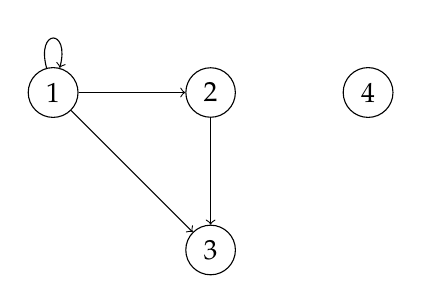
\begin{tikzpicture}[->,node distance=2cm]
  \node[draw,circle] (A) {$1$};
  \node[draw,circle] (B) [right of=A] {$2$};
  \node[draw,circle] (C) [below of=B] {$3$};
  \node[draw,circle] (D) [right of=B] {$4$};
  \draw (A) to [loop above]  (A);
  \draw (A) to  (B);
  \draw (A) to  (C);
  \draw (B) to  (C);
  \end{tikzpicture}
\intertext{Il diffère du graphe $\tuple{V', E}$ où
  $V' = \{1, 2, 3\}$, représenté ci-dessous :}
& 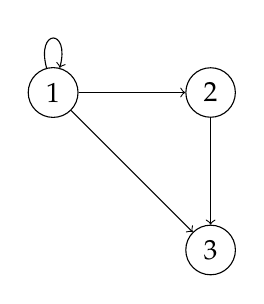
\begin{tikzpicture}[->,node distance=2cm]
  \node[draw,circle] (A) {$1$};
  \node[draw,circle] (B) [right of=A] {$2$};
  \node[draw,circle] (C) [below of=B] {$3$};
  \draw (A) to [loop above]  (A);
  \draw (A) to  (B);
  \draw (A) to  (C);
  \draw (B) to  (C);
  \end{tikzpicture}
\end{align*}
\end{ex}

\begin{prob}
Considérez la relation « inférieur ou égal à »~$\le$ sur l’ensemble
$\{1, 2, 3, 4\}$ comme un graphe et dessinez le diagramme correspondant.
\end{prob}


\endgroup
% END embedded source: content/sets-functions-relations/relations/graphs.tex



% BEGIN embedded source: content/sets-functions-relations/relations/trees.tex
\begingroup
\expandafter\def\csname ol@sectioncs\endcsname{section}
\def\olfilename{trees}


\olfileid[fr]{sfr}{rel}{tre}
\olsection{Arbres}

Un \emph{arbre} est un type particulier d’ordre partiel qui joue un rôle
important dans toutes les branches de la logique. Les arbres finis
apparaissent dès la logique élémentaire : les !!{formula}s peuvent ainsi
être analysées au moyen de leur décomposition en arbres syntaxiques,
et les !!{derivation}s, dans de nombreux systèmes de !!{derivation},
prennent elles aussi la forme d’arbres finis.
%
Les arbres infinis interviennent dès la démonstration des théorèmes
de complétude de la logique propositionnelle et de la logique du premier
ordre ; on les retrouve dans toute la logique mathématique.

La notion ensembliste d’arbre est étroitement liée à celle de la théorie
des graphes. Voici la représentation d’un arbre fini :

\begin{center}
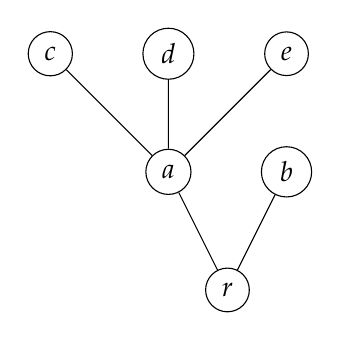
\begin{tikzpicture}[nodes={draw, circle}, -]
\node{$r$} [grow'=up]
    child { node {$a$}
        child { node {$c$} }
        child { node {$d$} }
        child { node {$e$} }
    }
    child { node {$b$} };
\end{tikzpicture}
\end{center}

Le nœud~$r$, situé tout en bas, est la racine. Tout nœud autre que $r$
possède exactement un nœud parent immédiatement au-dessous de lui.
On peut interpréter la relation entre un nœud~$x$ et un nœud~$y$ que
l’on atteint depuis~$x$ en suivant les arêtes vers le haut en disant
que $x$ est un \emph{ancêtre} de~$y$.

La relation d’ascendance dans un arbre est un ordre partiel strict.
Cela motive la définition ensembliste. Pour l’énoncer, nous avons besoin
de deux notions. Un \emph{plus petit élément} d’un ensemble~$A$
partiellement ordonné par~$\le$ est !!a{element} $x \in A$ tel que,
pour tout $y \in A$, on ait~$x \le y$. Un ensemble est \emph{bien ordonné}
par~$\le$ si chacune de ses parties non vides possède un plus petit élément.

\begin{defn}[Arbre]
Un \emph{arbre} est un couple $T = \tuple{A, \le}$ où $A$ est un ensemble
et $\le$ un ordre partiel sur~$A$ possédant un unique plus petit élément
$r \in A$, appelé la \emph{racine}, et tel que, pour tout $x \in A$,
l’ensemble $\Setabs{y}{y \le x}$ soit bien ordonné par~$\le$.
\end{defn}

\begin{defn}[Successeurs]
Soit $T = \tuple{A, \le}$ un arbre. Si $x,y \in A$, $x < y$ et
qu’il n’existe aucun $z \in A$ tel que $x < z < y$, on dit que $y$
est un \emph{successeur} de~$x$.
\end{defn}

Les successeurs de $x \in A$ sont aussi appelés ses \emph{enfants}.
Si $y$ est un successeur de~$x$, on dit que $x$ est le \emph{prédécesseur}
ou le \emph{parent} de~$y$.

\begin{prop}
Si $\tuple{A,\le}$ est un arbre, tout $x \in A$ autre que la racine
possède au plus un prédécesseur.
\end{prop}

\begin{proof}
Supposons $y_1 < x$, $y_2 < x$ et $y_1 \neq y_2$.
Alors $\{y_1, y_2\} \subseteq \Setabs{z}{z<x}$.
Puisque $\Setabs{z}{z<x}$ est bien ordonné par~$\le$, sa partie
$\{y_1, y_2\}$ possède un plus petit élément, qui est nécessairement
$y_1$ ou~$y_2$. Ainsi, $y_1 \le y_2$ ou $y_2 \le y_1$.
Or $y_1 \neq y_2$ par hypothèse ; on a donc $y_1 < y_2$ ou $y_2 < y_1$.
Comme $y_1 < x$ et $y_2 < x$, on en déduit que $y_1 < y_2 < x$
ou $y_2 < y_1 < x$. Les deux objets $y_1$ et $y_2$ ne peuvent donc
pas être tous deux des prédécesseurs de~$x$.
\end{proof}

\begin{defn}
Un arbre $T = \tuple{A, \le}$ est dit \emph{infini} si $A$ est infini,
et \emph{fini} sinon. Si chaque $x \in A$ possède un nombre fini
de successeurs, on dit que $T$ est \emph{à branchement fini}.
\end{defn}

\begin{defn}[Branches]
Soit $T = \tuple{A, \le}$ un arbre. Une \emph{branche} de~$T$ est une
chaîne maximale dans~$T$, c’est-à-dire un ensemble $B \subseteq A$
tel que, pour tous $x, y \in B$, on ait $x \le y$ ou $y \le x$,
et que, pour tout $z \in A \setminus B$, il existe $u \in B$ tel que
l’on n’ait ni $z \le u$ ni $u \le z$.\footnote{Correction éditoriale :
le domaine est bien celui de l’arbre. L’original écrivait ici la lettre
$X$, qui n’avait pas été définie, à la place de $A$.}
%
On note $[T]$ l’ensemble de toutes les branches de $T$.
\end{defn}

\begin{ex}
Un exemple classique d’arbre à branchement fini est l’\emph{arbre binaire
infini} des suites finies de $0$ et de~$1$, parfois noté $\{0,1\}^*$
ou~$\Bin^*$, muni de la relation de prolongement $\sqsubseteq$
(par exemple $101 \sqsubseteq 101101$). Comme on peut toujours prolonger
un mot binaire en lui ajoutant un $0$ ou un $1$ à la fin, cet arbre
contient une infinité d’éléments : chaque élément~$s$ possède exactement
deux successeurs, $s0$ et~$s1$. Sa racine est la suite vide $\emptyseq$.
\end{ex}

\begin{ex}
Plus généralement, l’ensemble des suites finies d’entiers naturels~$\Nat^*$,
muni de la relation de prolongement~$\sqsubseteq$, est aussi un arbre.
Il n’est manifestement pas à branchement fini : chaque $s \in \Nat^*$
possède une infinité de successeurs~$sn$, un pour chaque $n \in \Nat$.
Toute partie non vide $A \subseteq \Nat^*$ stable par passage aux
segments initiaux est un \emph{sous-arbre} de~$\Nat^*$.
(Autrement dit, si $s \in A$ et $s' \sqsubseteq s$, alors $s' \in A$.)
\footnote{Précision éditoriale : la condition « non vide » assure la
présence d’une racine, exigée par notre définition d’un arbre ;
l’original ne la précisait pas.}
Tout arbre fini peut être représenté par un sous-arbre fini de~$\Nat^*$.
\end{ex}

\begin{prop}[Lemme de K\H{o}nig]
Si $T = \tuple{A,\le}$ est un arbre infini à branchement fini,
alors $T$ possède une branche infinie.
\end{prop}

Un cas particulier du lemme de K\H{o}nig, couramment utilisé en théorie
de la calculabilité, est appelé le \emph{lemme faible de K\H{o}nig} :
tout sous-arbre infini de $\{0,1\}^*$ possède une branche infinie.


\endgroup
% END embedded source: content/sets-functions-relations/relations/trees.tex



% BEGIN embedded source: content/sets-functions-relations/relations/operations.tex
\begingroup
\expandafter\def\csname ol@sectioncs\endcsname{section}
\def\olfilename{operations}


\olfileid[fr]{sfr}{rel}{ops}
\olsection{Opérations sur les relations}

Il est souvent utile de modifier ou de combiner des relations.
Dans la \olref[sfr][rel][ord]{prop:stricttopartial}, nous avons considéré
leur \emph{réunion}, qui est simplement la réunion de deux relations
prises comme ensembles de couples. De même, dans la
\olref[sfr][rel][ord]{prop:partialtostrict}, nous avons considéré
leur différence ensembliste. Voici quelques autres opérations sur les relations.

\begin{defn}\ollabel{relationoperations}
Soient $R$ et $S$ des relations, et $A$ un ensemble quelconque.

La relation \emph{inverse} de $R$ est
$R^{-1} = \Setabs{\tuple{y, x}}{\tuple{x, y} \in R}$.

Le \emph{produit relatif} de $R$ et $S$ est
$(R \mid S) = \{\tuple{x, z} : \exists y(Rxy \land Syz)\}$.

La \emph{restriction} de $R$ à $A$ est
$\funrestrictionto{R}{A}= R \cap A^2$.

L’\emph{image} de $A$ par $R$ est
$\funimage{R}{A} = \{y : (\exists x \in A)Rxy\}$.
\end{defn}

\begin{ex}
Soit $S \subseteq \Int^2$ la relation de succession sur~$\Int$ :
$S = \Setabs{\tuple{x, y} \in \Int^2}{x + 1 = y}$.
Ainsi, $Sxy$ si et seulement si $x + 1 = y$.

$S^{-1}$ est la relation qui associe à chaque entier son prédécesseur,
soit $\Setabs{\tuple{x,y}\in\Int^2}{x -1 =y}$.

$S\mid S$ est $ \Setabs{\tuple{x,y}\in\Int^2}{x + 2 =y}$.

$\funrestrictionto{S}{\Nat}$ est la relation de succession sur~$\Nat$.

$\funimage{S}{\{1,2,3\}}$ est $\{2, 3, 4\}$.
\end{ex}

\begin{defn}[Clôture transitive]
Soit $R \subseteq A^2$ une relation binaire.\footnote{Précision de notation :
dans cette section, le signe plus en exposant désigne la clôture transitive.
Il n’a donc pas le sens local de clôture réflexive employé dans la
section sur les ordres. Les notations de l’original sont conservées.}

La \emph{clôture transitive} de~$R$ est
$R^+ = \bigcup_{0 < n \in \Nat} R^n$, où l’on définit par récurrence
$R^1 = R$ et $R^{n+1} = R^n \mid R$.

La \emph{clôture réflexive et transitive} de $R$ est
$R^* = R^+ \cup \Id{A}$.
\end{defn}

\begin{ex}
Reprenons la relation de succession $S \subseteq \Int^2$.
On a $S^2xy$ si et seulement si $x + 2 = y$, $S^3xy$ si et seulement si
$x + 3 = y$, etc. Ainsi, $S^+xy$ si et seulement si $x + n = y$
pour un certain $n \geq 1$. Autrement dit, $S^+xy$ si et seulement si
$x < y$, et $S^*xy$ si et seulement si $x \le y$.
\end{ex}

\begin{prob}
Montrez que la clôture transitive de $R$ est effectivement transitive.
\end{prob}


\endgroup
% END embedded source: content/sets-functions-relations/relations/operations.tex


\OLEndChapterHook


\endgroup
% END embedded source: content/sets-functions-relations/relations/relations-complete.tex


% BEGIN embedded source: content/sets-functions-relations/functions/functions.tex
\begingroup
\expandafter\def\csname ol@sectioncs\endcsname{section}
\def\olfilename{functions}


\olchapter{sfr}{fun}{Fonctions}


% BEGIN embedded source: content/sets-functions-relations/functions/function-basics.tex
\begingroup
\expandafter\def\csname ol@sectioncs\endcsname{section}
\def\olfilename{function-basics}


\olfileid[fr]{sfr}{fun}{bas}
\olsection{Notions de base}

\begin{explain}
Une \emph{fonction} associe à chaque !!{element} d’un ensemble donné
un !!{element} déterminé d’un autre ensemble donné, qui peut être le même.
Par exemple, l’opération qui consiste à ajouter~$1$ définit une fonction :
à chaque nombre~$n$, elle associe l’unique nombre~$n+1$.

Plus généralement, une fonction peut recevoir en entrée des couples,
des triplets, etc., et produire une sortie. L’arithmétique élémentaire
nous fournit de nombreuses fonctions familières : l’addition et la
multiplication, par exemple, reçoivent deux nombres et en renvoient un troisième.

Dans ce sens mathématique abstrait, une fonction est une \emph{boîte noire} :
seule compte la sortie associée à chaque entrée, et non la méthode
qui permet de la calculer.
\end{explain}

\begin{defn}[Fonction]
Une \emph{fonction} $f \colon A \to B$ associe à chaque !!{element}
de~$A$ un unique !!{element} de~$B$.

On appelle $A$ le \emph{domaine} de~$f$ et $B$ son \emph{ensemble d’arrivée}.
Les !!{element}s de~$A$ sont les entrées ou \emph{arguments} de~$f$.
L’!!{element} de~$B$ que~$f$ associe à un argument~$x$ est appelé
la \emph{valeur de~$f$} en~$x$ et se note~$f(x)$.

L’\emph{image} $\ran{f}$ de~$f$ est la partie de son ensemble d’arrivée
constituée des valeurs effectivement prises par~$f$ :
$\ran{f} = \Setabs{f(x)}{x \in A}$.
\end{defn}

Le diagramme de la \olref{fig:function} aide à se représenter une fonction.
L’ellipse de gauche représente son \emph{domaine}, celle de droite
son \emph{ensemble d’arrivée}. Chaque flèche part d’un \emph{argument}
du domaine et aboutit à la \emph{valeur} correspondante dans l’ensemble d’arrivée.

\begin{figure}
  \olasset{assets/diagrams/function.tikz}
  \caption{Une fonction associe à chaque !!{element} d’un ensemble
    !!a{element} d’un autre ensemble. Une flèche part d’un argument
    du domaine et aboutit à la valeur correspondante dans l’ensemble d’arrivée.}
  \ollabel{fig:function}
\end{figure}

\begin{ex}
La multiplication reçoit en entrée des couples d’entiers naturels et
renvoie des entiers naturels. Elle va donc de $\Nat \times \Nat$
(son domaine) dans $\Nat$ (son ensemble d’arrivée).
Son image est elle aussi $\Nat$, puisque tout $n \in \Nat$ est égal à
$n \times 1$.
\end{ex}

\begin{ex}
La multiplication est une fonction parce qu’elle associe à chaque entrée,
c’est-à-dire à chaque couple d’entiers naturels, une unique sortie :
$\times \colon \Nat^2 \to \Nat$. En revanche, associer à un entier
naturel~$n$ un réel~$x$ tel que $x^2 = n$ ne définit pas une fonction :
chaque entier strictement positif~$n$ possède deux racines carrées,
$\sqrt{n}$ et~$-\sqrt{n}$. On obtient une fonction en ne retenant que
la racine carrée positive ou nulle :
$\sqrt{\phantom{X}} \colon \Nat \to \Real$.
\footnote{Précision éditoriale : on inclut la racine nulle pour que
la fonction soit aussi définie en zéro, qui appartient à son domaine.}
\end{ex}

\begin{ex}
La relation qui associe à chaque étudiant d’un cours sa note finale est
une fonction : un étudiant ne peut pas recevoir deux notes finales
différentes pour un même cours. La relation qui associe à chaque étudiant
ses parents n’est pas une fonction : un étudiant peut avoir zéro, deux
ou davantage de parents.
\end{ex}

\begin{explain}
Pour définir une fonction, on peut préciser sa valeur pour chaque
argument possible. On peut le faire par une formule, par une méthode
de calcul ou par une liste des valeurs correspondant aux arguments.
Quelle que soit la méthode choisie, il faut s’assurer qu’à chaque
argument correspond une valeur et une seule.
\end{explain}

\begin{ex}
Soit $f \colon \Nat \to \Nat$ définie par $f(x) = x+1$.
Cette définition précise que $f$ reçoit des entiers naturels et renvoie
des entiers naturels : à tout entier naturel~$x$, elle associe son
successeur~$x+1$. Ici, l’ensemble d’arrivée $\Nat$ n’est pas l’image
de~$f$, car l’entier naturel~$0$ n’est le successeur d’aucun entier naturel.
L’image de~$f$ est l’ensemble des entiers strictement positifs, $\Int^{+}$.
\end{ex}

\begin{ex}\ollabel{examplefunext}
Soit $g \colon \Nat \to \Nat$ définie par $g(x) = x+2-1$.
C’est une fonction qui reçoit des entiers naturels et renvoie des
entiers naturels. À un entier naturel~$x$, elle associe le prédécesseur
du successeur du successeur de~$x$, soit $x+1$.
\footnote{Correction éditoriale : l’original appelait l’entrée
$n$ avant de la désigner par $x$ ; on emploie ici la même lettre.}
\end{ex}

\begin{explain}
Nous venons de considérer deux fonctions $f$ et $g$ données par des
\emph{définitions} différentes. Pourtant, il s’agit de la \emph{même fonction}.
Pour tout entier naturel~$n$, on a en effet
$f(n) = n+1 = n+2-1 = g(n)$. Autrement dit, nos définitions de $f$ et~$g$
décrivent la même correspondance au moyen d’équations différentes.
Nous utilisons donc implicitement un principe d’extensionnalité
pour les fonctions :
\[
  \text{si }\forall x\, f(x) = g(x)\text{, alors }f = g
\]
à condition que $f$ et~$g$ aient le même domaine et le même ensemble d’arrivée.
\end{explain}

\begin{ex}
On peut aussi définir une fonction par cas. Définissons par exemple
$h \colon \Nat \to \Nat$ par
\[
h(x) =
\begin{cases}
  \frac{x}{2} & \text{si $x$ est pair} \\
  \frac{x+1}{2} & \text{si $x$ est impair.}
\end{cases}
\]
Tout entier naturel étant pair ou impair, cette fonction renvoie toujours
un entier naturel. Dans une telle définition par cas disjoints, toute
entrée possible doit relever d’un cas et d’un seul. Il faut parfois
démontrer que les cas sont exhaustifs et mutuellement exclusifs.
\footnote{Précision éditoriale : l’original présente cette condition comme
une exigence générale. Des cas peuvent aussi se recouper, à condition
qu’ils attribuent la même valeur aux entrées communes ; toutes les entrées
doivent néanmoins être couvertes.}
\end{ex}


\endgroup
% END embedded source: content/sets-functions-relations/functions/function-basics.tex



% BEGIN embedded source: content/sets-functions-relations/functions/function-kinds.tex
\begingroup
\expandafter\def\csname ol@sectioncs\endcsname{section}
\def\olfilename{function-kinds}


\olfileid[fr]{sfr}{fun}{kin}
\olsection{Types de fonctions}

\begin{explain}
Il sera utile de classer certains types de fonctions que nous rencontrerons
fréquemment.

Commençons par les fonctions pour lesquelles chaque élément de l’ensemble
d’arrivée est une valeur prise par la fonction. Elles sont dites
!!{surjective}s et peuvent être représentées comme dans la
\olref{fig:surjective}.

\begin{figure}
  \olasset{assets/diagrams/surjective.tikz}
  \caption{Une fonction !!{surjective} prend pour valeur chaque
    !!{element} de son ensemble d’arrivée.}
  \ollabel{fig:surjective}
\end{figure}
\end{explain}

\begin{defn}[Fonction !!{surjective}]
Une fonction $f \colon A \rightarrow B$ est \emph{!!{surjective}} si et
seulement si $B$ est aussi l’image de~$f$ : pour tout $y \in B$, il existe
au moins un $x \in A$ tel que~$f(x) = y$. En symboles :
\[
  (\forall y \in B)(\exists x \in A)f(x) = y.
\]
On appelle une telle fonction !!a{surjection} de $A$ dans $B$.
\end{defn}

\begin{explain}
Pour montrer que $f$ est !!a{surjection}, il faut montrer que chaque
objet de son ensemble d’arrivée est égal à $f(x)$ pour une certaine
entrée $x$.

Toute fonction \emph{induit} une surjection. Étant donnée
$f \colon A \to B$, définissons $f' \colon A \to \ran{f}$ par
$f'(x) = f(x)$. Puisque $\ran{f}$ est \emph{par définition}
$\Setabs{f(x) \in B}{x \in A}$, la fonction $f'$ est nécessairement
!!a{surjection}.
\end{explain}

\begin{explain}
Toute fonction associe à chaque entrée possible une unique sortie.
Certaines fonctions ont en outre la propriété de ne jamais associer
la même sortie à deux entrées différentes. Elles sont dites
!!{injective}s et peuvent être représentées comme dans la
\olref{fig:injective}.
\begin{figure}
  \olasset{assets/diagrams/injective.tikz}
  \caption{Une fonction !!{injective} n’associe jamais la même valeur
    à deux arguments différents.}
  \ollabel{fig:injective}
\end{figure}
\end{explain}

\begin{defn}[Fonction !!{injective}]
Une fonction $f \colon A \rightarrow B$ est \emph{!!{injective}} si et
seulement si, pour chaque $y \in B$, il existe au plus un $x \in A$
tel que~$f(x) = y$. On appelle une telle fonction !!a{injection}
de $A$ dans~$B$.
\end{defn}

\begin{explain}
Pour montrer que $f$ est !!a{injection}, il faut montrer que,
pour tous les !!{element}s $x$ et $y$ de son domaine,
si $f(x)=f(y)$, alors $x=y$.
\end{explain}

\begin{ex}
La fonction constante $f\colon \Nat \to \Nat$ définie par $f(x) = 1$
n’est ni !!{injective} ni !!{surjective}.

La fonction identité $f\colon \Nat \to \Nat$ définie par $f(x) = x$
est à la fois !!{injective} et !!{surjective}.

La fonction successeur $f \colon \Nat \to \Nat$ définie par $f(x) = x+1$
est !!{injective}, mais n’est pas !!{surjective}.

La fonction $f \colon \Nat \to \Nat$ définie par
\[
  f(x) =
  \begin{cases}
    \frac{x}{2} & \text{si $x$ est pair} \\
    \frac{x+1}{2} & \text{si $x$ est impair.}
  \end{cases}
\]
est !!{surjective}, mais n’est pas !!{injective}.
\end{ex}

\begin{explain}
Nous aurons souvent besoin de fonctions à la fois !!{injective}s et
!!{surjective}s. On les dit !!{bijective}s ; elles se représentent
comme dans la \olref{fig:bijective}. Les !!{bijection}s sont aussi
parfois appelées \emph{correspondances biunivoques}, car elles font
correspondre de manière unique les éléments de l’ensemble d’arrivée
à ceux du domaine.
\begin{figure}
  \olasset{assets/diagrams/bijective.tikz}
  \caption{Une fonction !!{bijective} fait correspondre de manière unique
    les éléments de l’ensemble d’arrivée à ceux du domaine.}
  \ollabel{fig:bijective}
\end{figure}
\end{explain}

\begin{defn}[!!^{bijection}]
Une fonction $f \colon A \to B$ est \emph{!!{bijective}} si et seulement
si elle est à la fois !!{surjective} et !!{injective}.
On l’appelle !!a{bijection} de $A$ dans~$B$ (ou entre $A$ et~$B$).
\end{defn}


\endgroup
% END embedded source: content/sets-functions-relations/functions/function-kinds.tex



% BEGIN embedded source: content/sets-functions-relations/functions/functions-relations.tex
\begingroup
\expandafter\def\csname ol@sectioncs\endcsname{section}
\def\olfilename{functions-relations}


\olfileid[fr]{sfr}{fun}{rel}

\olsection{Les fonctions comme relations}

\begin{explain}
Une fonction qui envoie les !!{element}s de~$A$ sur des !!{element}s de~$B$
définit une relation entre $A$ et~$B$ : celle qui relie $x$ à $y$ si et
seulement si $f(x) = y$. On pourrait même, par exemple si l’on souhaite
réduire le nombre de notions fondamentales des mathématiques,
\emph{identifier} la fonction~$f$ à cette relation, c’est-à-dire à un
ensemble de couples. Une question se pose alors : quelles relations
définissent ainsi des fonctions ?
\end{explain}

\begin{defn}[Graphe d’une fonction] Soit $f\colon A \to B$ une fonction.
Le \emph{graphe} de~$f$ est la relation $R_f \subseteq A \times B$
définie par
\[
R_f = \Setabs{\tuple{x,y}}{f(x) = y}.
\]
\end{defn}

\begin{explain}
Par extensionnalité, le graphe d’une fonction est déterminé de manière
unique. De plus, l’extensionnalité des ensembles justifie immédiatement
le principe implicite d’extensionnalité des fonctions : deux fonctions
$f$ et~$g$ de mêmes domaine et ensemble d’arrivée sont identiques si
elles prennent les mêmes valeurs en chaque point de leur domaine.

De même, une relation « fonctionnelle » est le graphe d’une fonction.
\end{explain}

\begin{prop}\ollabel{prop:graph-function}
Soit $R \subseteq A \times B$ telle que :
\begin{enumerate}
\item si $Rxy$ et $Rxz$, alors $y = z$ ; et
\item pour tout $x \in A$, il existe $y \in B$ tel que
$\tuple{x,y} \in R$.
\end{enumerate}
Alors $R$ est le graphe de la fonction $f\colon A \to B$ définie par
$f(x) = y$ si et seulement si $Rxy$.
\end{prop}

\begin{proof}
Supposons qu’il existe $y$ tel que $Rxy$. S’il existait aussi $z \neq y$
tel que $Rxz$, la première condition sur~$R$ serait violée. Ainsi, un tel
$y$, lorsqu’il existe, est unique. La seconde condition en assure
l’existence pour chaque $x \in A$ ; la fonction $f$ est donc bien définie.
On a manifestement $R_f = R$.
\end{proof}

\begin{explain}
Toute fonction $f\colon A \to B$ possède un graphe : une relation
incluse dans $A \times B$, définie par $f(x) = y$. Réciproquement, toute
relation~$R \subseteq A \times B$ qui possède les propriétés de la
\olref{prop:graph-function} est le graphe d’une fonction~$f\colon A \to B$.
Ce lien étroit permet de considérer une fonction simplement comme son
graphe. Autrement dit, on peut identifier les fonctions à certaines
relations, donc à certains ensembles de couples.
\oliflabeldef{sfr:rel:ref:sec}{Il faut toutefois comprendre cette
« identification » dans l’esprit de la \olref[sfr][rel][ref]{sec} :
il ne s’agit pas d’une affirmation sur la métaphysique des fonctions,
mais du constat qu’il est commode de les \emph{traiter} comme certains
ensembles. Cela permet notamment d’envisager}{On peut ainsi envisager}
sur les fonctions des opérations analogues à celles que nous
avons effectuées sur les relations (voir la \olref[sfr][rel][ops]{sec}).
En particulier :
\end{explain}

\begin{defn}\ollabel{defn:funimage}
Soit $f\colon A \to B$ une fonction et soit $C\subseteq A$.

La \emph{restriction} de~$f$ à~$C$ est la
fonction~$\funrestrictionto{f}{C}\colon C \to B$ définie par
$(\funrestrictionto{f}{C})(x) = f(x)$ pour tout $x \in C$.
Autrement dit, $\funrestrictionto{f}{C} =
\Setabs{\tuple{x, y} \in R_f}{x \in C}$.

L’\emph{image} de~$C$ par~$f$ est $\funimage{f}{C} =
\Setabs{f(x)}{x \in C}$. On parle aussi de l’\emph{image directe}
de~$C$ par~$f$.
\end{defn}

\begin{explain}
Ces définitions donnent $\ran{f} = \funimage{f}{\dom{f}}$ pour toute
fonction~$f$.
\oliflabeldef{sfr:rel:ops:sec}{La notion d’image concorde avec celle
de la \olref[sfr][rel][ops]{sec} lorsqu’on identifie les fonctions à
leurs graphes. Pour la restriction, il faut distinguer les deux
conventions.\footnote{Précision éditoriale : l’original annonce un
accord des notions, mais la restriction d’une fonction à $C$ ne
restreint que la première coordonnée, tandis que la restriction d’une
relation définie précédemment intersecte son graphe avec $C^2$.
Ainsi, pour $f(n)=n+1$ sur $\Nat$ et $C=\{0\}$, la restriction
fonctionnelle a pour graphe $\{\tuple{0,1}\}$, alors que la restriction
relationnelle à $C$ est vide. Les deux coïncident lorsque
$\funimage{f}{C}\subseteq C$.}
Deux autres opérations, l’inversion et le produit relatif, demandent
quelques précisions supplémentaires. Nous les donnerons dans la
\olref[inv]{sec} et dans la \olref[cmp]{sec}.}{}
\end{explain}


\endgroup
% END embedded source: content/sets-functions-relations/functions/functions-relations.tex



% BEGIN embedded source: content/sets-functions-relations/functions/inverses.tex
\begingroup
\expandafter\def\csname ol@sectioncs\endcsname{section}
\def\olfilename{inverses}


\olfileid[fr]{sfr}{fun}{inv}
\olsection{Inverses des fonctions}

\begin{explain}
Nous envisageons les fonctions comme des correspondances entre objets.
Il est alors naturel de se demander si l’on peut « inverser » une telle
correspondance. Par exemple, on peut inverser la fonction successeur
$f(x) = x + 1$, au sens où la fonction $g(y) = y - 1$ « défait »
ce que fait $f$.

Il faut cependant être prudent. La définition de~$g$ donne bien une
fonction $\Int \to \Int$, mais elle ne définit pas une \emph{fonction}
$\Nat \to \Nat$, car $g(0) \notin \Nat$. Même dans un cas simple,
la possibilité d’inverser une fonction ne va donc pas de soi :
elle peut dépendre du domaine et de l’ensemble d’arrivée.

La notion d’inverse d’une fonction permet de préciser cette idée.
\end{explain}

\begin{defn}
Une fonction $g\colon B \to A$ est un \emph{inverse} d’une fonction
$f\colon A \to B$ si $f(g(y)) = y$ et $g(f(x)) = x$ pour tous
$x \in A$ et $y \in B$.
\end{defn}

Si $f$ admet un inverse~$g$, on écrit souvent $f^{-1}$ au lieu de~$g$.

\begin{explain}
Déterminons maintenant quelles fonctions admettent un inverse.
Pour inverser $f\colon A \to B$, on peut envisager la fonction
$g\colon B \to A$ « définie par »
\[
g(y) = \text{« le » $x$ tel que $f(x) = y$.}
\]
Mais les guillemets autour de « définie par » et de « le » signalent
qu’il ne s’agit pas encore d’une définition valable en toute généralité.
Pour définir ainsi une fonction, il faut qu’il existe un et un seul~$x$
tel que $f(x) = y$ : la valeur de~$g$ doit être déterminée de manière
unique. Elle doit en outre être définie pour chaque $y \in B$.
S’il existe $x_1,x_2 \in A$ tels que $x_1 \neq x_2$ mais
$f(x_1) = f(x_2)$, la valeur $g(y)$ n’est pas déterminée de manière
unique pour $y = f(x_1) = f(x_2)$. Et s’il n’existe aucun~$x$ tel que
$f(x) = y$, la valeur $g(y)$ n’est pas définie du tout.
Autrement dit, pour que $g$ soit ainsi définie, il faut que $f$ soit
à la fois !!{injective} et !!{surjective}.

Procédons par étapes. Séparons la question en deux : étant donnée une
fonction~$f\colon A \to B$, quand existe-t-il une fonction
$g\colon B \to A$ telle que $g(f(x)) = x$ ? Une telle fonction $g$
« défait » ce que fait $f$ ; on l’appelle un \emph{inverse à gauche}
de~$f$. D’autre part, quand existe-t-il une fonction $h\colon B \to A$
telle que $f(h(y)) = y$ ? Une telle fonction $h$ est un
\emph{inverse à droite} de~$f$ : cette fois, $f$ « défait » ce que fait~$h$.
\end{explain}

\begin{prop}
Si $f\colon A \to B$ est !!{injective} et si $A$ est non vide,
alors $f$ possède un \emph{inverse à gauche}~$g\colon B \to A$ tel que
$g(f(x)) = x$ pour tout $x \in A$.\footnote{Précision éditoriale :
l’hypothèse que le domaine est non vide manque dans l’original.
L’unique fonction de $\emptyset$ vers un ensemble non vide est injective,
mais aucune fonction en sens inverse n’existe. Si les deux ensembles
sont vides, leur unique fonction est son propre inverse.}
\end{prop}

\begin{proof}
Supposons $f\colon A \to B$ !!{injective}, avec $A$ non vide.
Considérons $y \in B$. Si $y \in \ran{f}$, il existe $x \in A$ tel que
$f(x) = y$. L’injectivité de $f$ assure l’unicité d’un tel~$x \in A$.
On peut donc poser $g(y) = x$ : $g(y)$ est « le » $x \in A$ tel que
$f(x) = y$. Si $y \notin \ran{f}$, on peut l’envoyer sur n’importe
quel~$a \in A$. Fixons donc $a \in A$ et définissons $g\colon B \to A$ par
\[
g(y) = \begin{cases}
    x & \text{si $f(x) = y$}\\
    a & \text{si $y \notin \ran{f}$.}
\end{cases}
\]
La fonction est définie pour tout $y \in B$ : dans le premier cas,
il existe exactement un $x \in A$ tel que $f(x) = y$, et dans le second
cas la valeur est $a$. Par définition, si $y = f(x)$, alors $g(y) = x$,
c’est-à-dire $g(f(x)) = x$.
\end{proof}

\begin{prob}
Montrez que, si $f\colon A \to B$ possède un inverse à gauche~$g$,
alors $f$ est !!{injective}.
\end{prob}

\begin{prop}
Si $f\colon A \to B$ est !!{surjective}, alors $f$ possède un
\emph{inverse à droite}~$h\colon B \to A$ tel que $f(h(y)) = y$
pour tout~$y \in B$.
\end{prop}

\begin{proof}
Supposons que $f\colon A \to B$ soit !!{surjective}. Considérons
$y \in B$. La surjectivité de $f$ assure l’existence de $x_y \in A$
tel que $f(x_y) = y$. On peut alors poser $h(y) = x_y$ : pour chaque
$y \in B$, on choisit un $x \in A$ tel que $f(x) = y$.
Puisque $f$ est !!{surjective}, il existe toujours au moins un tel
objet.\footnote{La surjectivité de $f$ assure que, pour chaque~$y \in B$,
l’ensemble $\Setabs{x}{f(x) = y}$ est non vide. Définir~$h$ exige de
choisir un seul $x$ dans chacun de ces ensembles. Il ne va pas de soi
que cela soit toujours possible : la possibilité d’effectuer ces choix
est posée comme un axiome. Autrement dit, cette proposition suppose
l’axiome du choix, une question que nous
\oliflabeldef{sth:choice::chap}{reprendrons dans le
\olref[sth][choice][]{chap}}{laisserons ici de côté}.
Dans de nombreux cas particuliers, par exemple lorsque $A = \Nat$,
lorsque $A$ est fini ou lorsque $f$ est !!{bijective}, l’axiome du choix
n’est toutefois pas nécessaire. Dans ce dernier cas, pour chaque $y \in B$,
l’ensemble $\Setabs{x}{f(x) = y}$ possède exactement un !!{element} :
il n’y a donc aucun choix à faire.}
Par définition, si $x = h(y)$, alors $f(x) = y$ ; ainsi,
pour tout $y \in B$, on a $f(h(y)) = y$.
\end{proof}

\begin{prob}
Montrez que, si $f\colon A \to B$ possède un inverse à droite~$h$,
alors $f$ est !!{surjective}.
\end{prob}

\begin{explain}
En combinant les idées de la démonstration précédente, on obtient que
toute !!{bijection} possède un inverse : une même fonction est à la fois
un inverse à gauche et un inverse à droite de~$f$.
\end{explain}

\begin{prop}\ollabel{prop:bijection-inverse}
Si $f\colon A \to B$ est !!{bijective}, il existe une
fonction~$f^{-1}\colon B \to A$ telle que, pour tout $x \in A$,
$f^{-1}(f(x)) = x$ et, pour tout $y \in B$, $f(f^{-1}(y)) = y$.
\end{prop}

\begin{proof}
La démonstration est laissée en exercice.
\end{proof}

\begin{prob}
Démontrez la \olref[sfr][fun][inv]{prop:bijection-inverse}.
Il faut définir~$f^{-1}$, montrer qu’il s’agit d’une fonction, puis
qu’elle est un inverse de~$f$, c’est-à-dire que $f^{-1}(f(x)) = x$ et
$f(f^{-1}(y)) = y$ pour tous $x \in A$ et $y \in B$.
\end{prob}

\begin{explain}
On peut obtenir des inverses d’une manière légèrement plus générale.
Nous avons vu dans la \olref[kin]{sec} que toute fonction $f$ induit
!!a{surjection} $f'\colon A \to \ran{f}$, en posant $f'(x) = f(x)$
pour tout $x \in A$. Si $f$ est !!{injective}, $f'$ est manifestement
!!{bijective} et possède donc un inverse, d’après la
\olref{prop:bijection-inverse}. Cet inverse est unique, comme le
montrera la \olref{prop:inverse-unique}.\footnote{Note de traduction :
l’original attribue aussi l’unicité à la proposition d’existence.
Le renvoi à la proposition d’unicité, démontrée plus bas, est précisé ici.}
Par un très léger abus de notation,
on appelle parfois simplement l’inverse de $f'$ « l’inverse de~$f$ ».
\end{explain}

\begin{prop}\ollabel{prop:left-right}%
Montrez que, si $f\colon A \to B$ possède un inverse à gauche~$g$
et un inverse à droite~$h$, alors $h = g$.
\end{prop}

\begin{proof}
La démonstration est laissée en exercice.
\end{proof}

\begin{prob}
Démontrez la \olref[sfr][fun][inv]{prop:left-right}.
\end{prob}

\begin{prop}\ollabel{prop:inverse-unique}
Toute fonction~$f$ possède au plus un inverse.
\end{prop}

\begin{proof}
Supposons que $g$ et $h$ soient deux inverses de~$f$. En particulier,
$g$ est un inverse à gauche de~$f$ et $h$ un inverse à droite.
Par la \olref{prop:left-right}, on a $g = h$.
\end{proof}


\endgroup
% END embedded source: content/sets-functions-relations/functions/inverses.tex



% BEGIN embedded source: content/sets-functions-relations/functions/composition.tex
\begingroup
\expandafter\def\csname ol@sectioncs\endcsname{section}
\def\olfilename{composition}


\olfileid[fr]{sfr}{fun}{cmp}
\olsection{Composition des fonctions}

\begin{explain}
\oliflabeldef{sfr:fun:inv:sec}{Nous avons vu dans la \olref[inv]{sec}
que l’inverse~$f^{-1}$ d’!!a{bijection}~$f$ est lui-même une fonction.
Une autre opération sur les fonctions est la composition : on}{On}
peut définir une nouvelle fonction en composant deux fonctions $f$ et~$g$,
c’est-à-dire en appliquant d’abord $f$, puis~$g$. Cela exige que les
images et les domaines soient compatibles : l’image de~$f$ doit être
incluse dans le domaine de~$g$.
\oliflabeldef{sfr:rel:ops:sec}{Cette opération est l’analogue, pour les
fonctions, du produit relatif des relations défini dans la
\olref[rel][ops]{sec}.}{}

Un diagramme peut aider à comprendre la composition. La
\olref{fig:composition} représente deux fonctions $f\colon A \to B$
et $g\colon B \to C$, ainsi que leur composée~$(\comp{f}{g})$.
La fonction $(\comp{f}{g})\colon A \to C$ associe à chaque !!{element}
de~$A$ un !!{element} de~$C$. Voici comment déterminer lequel :
étant donnée une entrée $x \in A$, on applique d’abord $f$ à~$x$,
ce qui donne $f(x) = y \in B$, puis on applique $g$ à~$y$,
ce qui donne $g(f(x)) = g(y) = z \in C$.
\begin{figure}
  \olasset[2\olphotowidth]{assets/diagrams/composition.tikz}
  \caption{La composée $g \circ f$ de deux fonctions $f$ et~$g$.}
  \ollabel{fig:composition}
\end{figure}
\end{explain}

\begin{defn}[Composition]
Soient $f\colon A \to B$ et $g\colon B \to C$ deux fonctions.
La \emph{composée} de $f$ suivie de~$g$ est
$\comp{f}{g}\colon A \to C$, définie par
$(\comp{f}{g})(x) = g(f(x))$.
\end{defn}

\begin{ex}
Considérons les fonctions $f(x) = x + 1$ et $g(x) = 2x$.
Puisque $(\comp{f}{g})(x) = g(f(x))$, il faut, pour chaque entrée~$x$,
prendre d’abord son successeur, puis multiplier le résultat par deux.
La composée est donc donnée par $(\comp{f}{g})(x) = 2(x+1)$.
\end{ex}

\begin{prob}
Montrez que, si $f\colon A \to B$ et $g\colon B \to C$ sont toutes deux
!!{injective}s, alors $\comp{f}{g}\colon A \to C$ est !!{injective}.
\end{prob}

\begin{prob}
Montrez que, si $f\colon A \to B$ et $g\colon B \to C$ sont toutes deux
!!{surjective}s, alors $\comp{f}{g}\colon A \to C$ est !!{surjective}.
\end{prob}

\begin{prob}
Soient $f\colon A \to B$ et $g\colon B \to C$. Montrez que le graphe
de $\comp{f}{g}$ est $R_f \mid R_g$.
\end{prob}


\endgroup
% END embedded source: content/sets-functions-relations/functions/composition.tex


%\olimport{isomorphic-functions}


% BEGIN embedded source: content/sets-functions-relations/functions/partial-functions.tex
\begingroup
\expandafter\def\csname ol@sectioncs\endcsname{section}
\def\olfilename{partial-functions}


\olfileid[fr]{sfr}{fun}{par}

\olsection{Fonctions partielles}

\begin{explain}
Il est parfois utile d’assouplir la définition d’une fonction en
n’exigeant plus que sa valeur soit définie pour toute entrée possible.
On parle alors de \emph{fonctions partielles}.
\end{explain}

\begin{defn}
Une \emph{fonction partielle} $f\colon A \pto B$ est une correspondance
qui associe à chaque !!{element} de~$A$ au plus un !!{element} de~$B$.
Si $f$ associe un élément de~$B$ à $x \in A$, on dit que $f(x)$ est
\emph{définie} ; sinon, on dit qu’elle est \emph{non définie}.
Si $f(x)$ est définie, on écrit $f(x) \fdefined$ ; sinon,
on écrit $f(x) \fundefined$. Le \emph{domaine} d’une fonction
partielle~$f$ est la partie de~$A$ où elle est définie :
$\dom{f} = \Setabs{x \in A}{f(x) \fdefined}$.
\end{defn}

\begin{ex}
Toute fonction $f\colon A \to B$ est aussi une fonction partielle.
Les fonctions partielles définies partout sur~$A$, c’est-à-dire celles
que nous avons jusqu’ici simplement appelées des fonctions, sont aussi
appelées des fonctions \emph{totales}.
\end{ex}

\begin{ex}
La fonction partielle $f\colon \Real \pto \Real$ donnée par $f(x) = 1/x$
n’est pas définie pour $x = 0$, et elle est définie partout ailleurs.
\end{ex}

\begin{prob}
Étant donnée $f\colon A \pto B$, définissons la fonction partielle
$g\colon B \pto A$ de la manière suivante : pour tout $y \in B$,
s’il existe un unique $x \in A$ tel que $f(x) = y$, on pose $g(y) = x$ ;
sinon, $g(y) \fundefined$. Montrez que, si $f$ est injective, alors
$g(f(x)) = x$ pour tout $x \in \dom{f}$, et $f(g(y)) = y$ pour tout
$y \in \ran{f}$.
\end{prob}

\begin{defn}[Graphe d’une fonction partielle]
Soit $f\colon A \pto B$ une fonction partielle. Le \emph{graphe} de~$f$
est la relation $R_f \subseteq A \times B$ définie par
\[
R_f = \Setabs{\tuple{x,y}}{f(x) = y}.
\]
\end{defn}

\begin{prop}
Supposons que $R \subseteq A \times B$ vérifie la propriété suivante :
chaque fois que $Rxy$ et $Rxy'$, on a $y = y'$.
Alors $R$ est le graphe de la fonction partielle $f\colon A \pto B$
définie ainsi : s’il existe $y$ tel que $Rxy$, on pose $f(x) = y$ ;
sinon, $f(x) \fundefined$. Si $R$ est de plus \emph{sérielle},
c’est-à-dire si, pour chaque $x \in A$, il existe $y \in B$ tel que
$Rxy$, alors $f$ est totale.
\end{prop}

\begin{proof}
Supposons qu’il existe $y$ tel que $Rxy$. S’il existait aussi $y' \neq y$
tel que $Rxy'$, la condition sur $R$ serait violée. Ainsi, un tel $y$,
lorsqu’il existe, est unique ; $f$ est donc bien définie.
On a manifestement $R_f = R$, et $f$ est totale si~$R$ est sérielle.
\end{proof}


\endgroup
% END embedded source: content/sets-functions-relations/functions/partial-functions.tex


\OLEndChapterHook


\endgroup
% END embedded source: content/sets-functions-relations/functions/functions.tex


% BEGIN embedded source: content/sets-functions-relations/size-of-sets/size-of-sets-complete.tex
\begingroup
\expandafter\def\csname ol@sectioncs\endcsname{section}
\def\olfilename{size-of-sets-complete}


\olchapter{sfr}{siz}{La taille des ensembles}

\begin{editorial}
Ce chapitre traite des énumérations, de la dénombrabilité et de la
non-dénombrabilité. Plusieurs sections existent en deux versions :
une présentation plus élémentaire, où les énumérations sont des
listes, ou des surjections depuis $\PosInt$, et une présentation
plus abstraite, où les énumérations sont des bijections avec
$\Nat$ ou un segment initial.\footnote{Précision éditoriale :
l'original abrège ici la seconde définition en ne mentionnant que
$\Nat$ ; les segments initiaux sont nécessaires pour les ensembles
finis et figurent dans la définition détaillée.}
\end{editorial}


% BEGIN embedded source: content/sets-functions-relations/size-of-sets/introduction.tex
\begingroup
\expandafter\def\csname ol@sectioncs\endcsname{section}
\def\olfilename{introduction}


\olfileid[fr]{sfr}{siz}{int}

\olsection{Introduction}

Lorsque Georg Cantor développa la théorie des ensembles dans les années
1870, il cherchait notamment à faire admettre l’idée d’une collection
infinie : un infini en acte, comme l’auraient dit les penseurs médiévaux.
Son étude de la \emph{taille} des ensembles joua un rôle essentiel
dans cette démarche. Si $a$, $b$ et $c$ sont tous distincts, l’ensemble
$\{a, b, c\}$ est intuitivement \emph{plus grand} que $\{a, b\}$.
Mais qu’en est-il des ensembles infinis ? Ont-ils tous la même taille ?
Il se trouve que non.

La première idée importante est celle d’énumération. On peut dresser
la liste des !!{element}s de tout ensemble fini. Pour certains ensembles
infinis, on peut aussi dresser une telle liste, à condition de permettre
qu’elle soit elle-même infinie. Ces ensembles sont dits !!{enumerable}s.
Le résultat surprenant de Cantor, que nous comprendrons pleinement
à la fin de ce chapitre, est que certains ensembles infinis ne sont pas
!!{enumerable}s.


\endgroup
% END embedded source: content/sets-functions-relations/size-of-sets/introduction.tex



% BEGIN embedded source: content/sets-functions-relations/size-of-sets/enumerability.tex
\begingroup
\expandafter\def\csname ol@sectioncs\endcsname{section}
\def\olfilename{enumerability}


\olfileid[fr]{sfr}{siz}{enm}

\olsection{Énumérations et ensembles \usetoken{p}{enumerable}}

\begin{editorial}
Cette section définit les énumérations d’ensembles comme des surjections
de $\PosInt$ sur ces ensembles. Elle procède progressivement, pour
les lecteurs ayant peu de connaissances mathématiques préalables.
La \olref[enm-alt]{sec} propose une présentation plus concise, fondée
sur une autre définition : une bijection avec $\Nat$ ou avec un segment
initial. Dans cette édition, \emph{au plus dénombrable} inclut les
ensembles finis et l’ensemble vide.\footnote{Convention éditoriale :
le mot anglais \emph{enumerable} est employé ici sans condition de
calculabilité. Une énumération n’est pas nécessairement donnée par
un algorithme ; il ne s’agit pas d’énumérabilité calculable.}
\end{editorial}

\begin{explain}
Nous avons déjà donné des exemples d’ensembles en dressant la liste
de leurs !!{element}s. Examinons plus généralement comment et dans
quels cas on peut dresser la liste des !!{element}s d’un ensemble,
même infini.
\end{explain}

\begin{defn}[Énumération : définition informelle]
Informellement, une \emph{énumération} d’un ensemble~$A$ est une liste,
éventuellement infinie, d’!!{element}s de~$A$, dans laquelle chaque
!!{element} de $A$ apparaît à une position finie. Si $A$ possède
une énumération, on dit qu’il est \emph{!!{enumerable}}.
\end{defn}

\begin{explain}
Précisons quelques points sur les énumérations :
\begin{enumerate}
\item Sauf pour la liste vide, admise ci-dessous, les listes considérées
  ont un premier !!{element}, et chaque !!{element} autre que le premier
  possède un unique !!{element} immédiatement avant lui. Nous exigeons
  en outre qu’il n’y ait qu’un nombre fini d’éléments entre le premier
  !!{element} et tout autre !!{element} de la liste. Ainsi, chaque
  !!{element} de l’énumération occupe une position finie : le premier
  est en position~$1$, le deuxième en position~$2$, etc.\footnote{Précision
  éditoriale : l’original présente ces deux conditions comme équivalentes.
  L’existence d’un prédécesseur immédiat ne suffit pas, à elle seule,
  à assurer que chaque terme occupe une position finie.}
\item Un même ensemble~$A$ peut avoir plusieurs énumérations, où les
  !!{element}s apparaissent dans des ordres différents : $4$, $1$,
  $25$, $16$,~$9$ énumère les cinq premiers carrés strictement positifs
  aussi bien que $1$, $4$, $9$, $16$,~$25$.
\item Une liste avec répétitions reste une énumération : $1$, $1$, $2$,
  $2$, $3$, $3$,~\dots{} énumère le même ensemble que $1$, $2$,
  $3$,~\dots
\item L’ordre et les répétitions \emph{comptent}, en revanche, lorsqu’on
  précise une énumération particulière. On peut énumérer les entiers
  strictement positifs en commençant par $1$, $2$, $3$, $1$, \dots{},
  mais la règle est plus facile à reconnaître dans l’énumération
  habituelle $1$, $2$, $3$, $4$,~\dots
\item Une énumération non vide doit avoir un début : \dots, $3$, $2$,
  $1$ n’est pas une énumération des entiers strictement positifs, car
  cette liste n’a pas de premier !!{element}. Pour comprendre le lien
  avec la définition informelle, demandez-vous à quelle position
  de cette liste se trouverait le nombre 76.
\item La liste suivante n’énumère pas non plus les entiers strictement
  positifs : $1$, $3$, $5$, \dots, $2$, $4$, $6$, \dots\@ Les nombres
  pairs y seraient placés aux positions $\infty + 1$, $\infty + 2$,
  $\infty + 3$, et non à des positions finies.
\item L’ensemble vide est au plus dénombrable : la liste vide l’énumère !
\end{enumerate}
\end{explain}

\begin{prop}
Si $A$ possède une énumération, il en possède une sans répétitions.
\end{prop}

\begin{proof}
Si $A$ est vide, sa liste vide ne comporte aucune répétition.
Sinon, supposons que $A$ possède une énumération $x_1$, $x_2$, \dots{}, dont
chaque terme $x_i$ est un !!{element} de~$A$. On peut supprimer les
répétitions en retirant les termes déjà rencontrés : on conserve $x_i$
s’il ne figure pas parmi $x_1$, \dots, $x_{i-1}$, et on le retire
s’il apparaît déjà parmi $x_1$, \dots,~$x_{i-1}$.
\end{proof}

Ce dernier raisonnement montre que, pour mieux comprendre les
énumérations et les ensembles !!{enumerable}s, puis démontrer des
résultats à leur sujet, il nous faut une définition plus précise.
La voici.

\begin{defn}[Énumération : définition formelle]
Une \emph{énumération} d’un ensemble $A \neq \emptyset$ est une
fonction !!{surjective} $f \colon \PosInt \to A$.
\end{defn}

\begin{explain}
Vérifions que cette définition formelle correspond à la définition
informelle par une liste éventuellement infinie. Toute fonction
!!{surjective} de $\PosInt$ dans un ensemble~$A$ énumère~$A$ : elle
détermine la liste $f(1)$, $f(2)$, $f(3)$, \dots. La surjectivité de $f$
assure que chaque !!{element} de~$A$ est la valeur de~$f(n)$ pour
un certain~$n \in \PosInt$. Chaque !!{element} apparaît donc à une
position finie. La fonction n’étant pas nécessairement !!{injective},
la liste peut comporter des répétitions ; nous avons vu que cela
est permis.

Réciproquement, à partir d’une liste qui énumère tous les !!{element}s
de~$A$, on peut définir une fonction !!{surjective} $f\colon \PosInt \to A$
en prenant pour $f(n)$ le $n$-ième !!{element} de la liste, ou son dernier
!!{element} si elle n’a pas de $n$-ième !!{element}. Cette construction
échoue seulement lorsque $A$ est vide, et que la liste est donc vide.
Ainsi, toute liste non vide qui énumère~$A$ détermine une fonction
!!{surjective} $f\colon \PosInt \to A$.
\end{explain}

\begin{defn}
  \ollabel{defn:enumerable}
Un ensemble~$A$ est !!{enumerable} si et seulement s’il est vide
ou possède une énumération.
\end{defn}

\begin{ex}
Pour énumérer les entiers strictement positifs ($\PosInt$), il suffit
de la fonction identité $f(n) = n$. La fonction $g(n) = n - 1$
énumère les entiers naturels $\Nat$.
\end{ex}

\begin{ex}
Les fonctions $f\colon \PosInt \to \PosInt$ et
$g \colon \PosInt \to \PosInt$ définies par
\begin{align*}
f(n) & = 2n \text{ et}\\
g(n) & = 2n - 1
\end{align*}
énumèrent respectivement les entiers pairs strictement positifs et
les entiers impairs strictement positifs. Cependant, aucune des deux
n’énumère $\PosInt$, car aucune n’est !!{surjective} sur cet ensemble.
\end{ex}

\begin{prob}
Définissez une énumération des carrés strictement positifs
$1$, $4$, $9$, $16$, \dots
\end{prob}

\begin{ex}
La fonction $f(n) = (-1)^{n} \lceil \frac{(n-1)}{2}\rceil$ énumère
l’ensemble des entiers relatifs~$\Int$. Ici, $\lceil x \rceil$ désigne
le \emph{plafond} de~$x$, c’est-à-dire le plus petit entier supérieur
ou égal à~$x$. Les valeurs de $f$ passent alternativement des entiers
positifs aux entiers négatifs :
\[
\begin{array}{c c c c c c c c}
f(1) & f(2) & f(3) & f(4) & f(5) & f(6) & f(7) & \dots \\ \\
- \lceil \tfrac{0}{2} \rceil & \lceil \tfrac{1}{2}\rceil & - \lceil \tfrac{2}{2} \rceil & \lceil \tfrac{3}{2} \rceil & - \lceil \tfrac{4}{2} \rceil  & \lceil \tfrac{5}{2}
\rceil & - \lceil \tfrac{6}{2} \rceil & \dots \\ \\
0 & 1 & -1 & 2 & -2 & 3 & -3 & \dots
\end{array}
\]
\footnote{Correction éditoriale : on rétablit la valeur $-3$ sous
$f(7)$ dans la dernière ligne du tableau ; elle manquait dans l’original.}
On peut également définir $f$ par cas :
\[
f(n) = \begin{cases}
  0 & \text{si $n = 1$}\\
  n/2 & \text{si $n$ est pair}\\
  -(n-1)/2 & \text{si $n$ est impair et $>1$}
  \end{cases}
\]
\end{ex}

\begin{prob}
Montrez que, si $A$ et $B$ sont !!{enumerable}s, $A \cup B$ l’est aussi.
Pour cela, supposez données des fonctions !!{surjective}s
$f\colon \PosInt \to A$ et $g\colon \PosInt \to B$. Définissez une
fonction~$h\colon \PosInt \to A \cup B$ et montrez qu’elle est
!!{surjective}. Traitez aussi les cas où $A$ ou~$B = \emptyset$.
\end{prob}

\begin{prob}
Montrez que, si $B \subseteq A$ et $A$ est !!{enumerable}, $B$ l’est
aussi. Supposez pour cela donnée une fonction !!{surjective}
$f\colon \PosInt \to A$. Définissez une fonction~$g\colon \PosInt \to B$
et montrez qu’elle est !!{surjective}. Que se passe-t-il si
$B = \emptyset$ ?
\end{prob}

\begin{prob}
Montrez par récurrence sur $n$ que, si $A_1$, $A_2$, \dots, $A_n$ sont
tous !!{enumerable}s, $A_1 \cup \dots \cup A_n$ l’est aussi.
Vous pouvez admettre que la réunion de deux ensembles $A$ et~$B$
!!{enumerable}s, $A \cup B$, est !!{enumerable}.
\end{prob}

Lorsqu’on dresse la liste des !!{element}s d’un ensemble, il paraît
peut-être plus naturel de commencer par le premier. Les mathématiciens
utilisent pourtant volontiers les entiers naturels~$\Nat$ pour
numéroter les objets : ils parlent du terme d’indice~$0$, puis des
termes d’indices~$1$, $2$, etc. On peut donc aussi définir une énumération
comme une fonction !!{surjective} de $\Nat$ dans~$A$.
Les deux définitions sont équivalentes.

\begin{prop}\ollabel{prop:enum-shift}
Il existe !!a{surjection} $f\colon \PosInt \to A$ si et seulement
s’il existe !!a{surjection} $g\colon \Nat \to A$.
\end{prop}

\begin{proof}
Étant donnée !!a{surjection} $f\colon \PosInt \to A$, posons
$g(n) = f(n+1)$ pour tout $n \in \Nat$. On vérifie aisément que
$g\colon \Nat \to A$ est !!{surjective}. Réciproquement, étant donnée
!!a{surjection} $g\colon \Nat \to A$, posons $f(n) = g(n-1)$.
\end{proof}

On obtient ainsi le résultat suivant :

\begin{cor}\ollabel{cor:enum-nat}
Un ensemble $A$ est !!{enumerable} si et seulement s’il est vide
ou s’il existe une fonction !!{surjective} $f\colon \Nat \to A$.
\end{cor}

Nous avons vu qu’on peut transformer une liste d’!!{element}s
d’un ensemble~$A$ en une liste sans répétitions. Cela vaut aussi pour
les énumérations au sens formel, mais l’énoncé et la démonstration
demandent davantage de soin. Toute fonction $f\colon \PosInt \to A$
doit être définie pour chaque $n \in \PosInt$. Si $A$ ne possède
qu’un nombre fini d’!!{element}s, une fonction définie sur tous les
!!{element}s de $\PosInt$ ne peut prendre pour valeurs tous les
!!{element}s de~$A$ sans jamais se répéter. Lorsque la liste sans
répétitions est finie, il faut donc choisir pour~$f$ un autre domaine,
qui ne possède qu’un nombre fini d’!!{element}s. L’absence de répétitions
signifie que $f$ est !!{injective}. Puisqu’elle est aussi !!{surjective},
nous cherchons !!a{bijection} entre $\{1, \dots, n\}$ ou $\PosInt$ et~$A$.

\begin{prop}\ollabel{prop:enum-bij}
Si $f\colon \PosInt \to A$ est !!{surjective}, c’est-à-dire si elle
énumère~$A$, il existe !!a{bijection} $g\colon Z \to A$, où $Z$ est
soit~$\PosInt$, soit $\{1, \dots, n\}$ pour un certain~$n \in \PosInt$.
\end{prop}

\begin{proof}
Définissons $g$ par récurrence. Posons $g(1) = f(1)$. Une fois la valeur
$g(i)$ définie, prenons pour $g(i+1)$ la première valeur de la liste $f(1)$,
$f(2)$, \dots{} qui ne figure pas déjà parmi $g(1)$, \dots, $g(i)$,
s’il en existe une. Si $A$ possède exactement $n$ !!{element}s,
toutes les valeurs $g(1)$, \dots, $g(n)$ sont définies, ce qui donne
une fonction $g\colon \{1, \dots, n\} \to A$. Si $A$ possède une
infinité d’!!{element}s, alors, pour tout $i$, l’énumération $f(1)$,
$f(2)$, \dots{} contient un !!{element} de~$A$ qui ne figure pas encore
parmi $g(1)$, \dots, $g(i)$. On obtient alors une fonction
$g\colon \PosInt \to A$.

La fonction $g$ est !!{surjective} : tout élément de~$A$ apparaît
parmi $f(1)$, $f(2)$, \dots{}, puisque $f$ est !!{surjective}, et finit
donc par être une valeur $g(i)$. Elle est aussi !!{injective} : s’il
existait $j < i$ tel que $g(j) = g(i)$, la valeur $g(i)$ figurerait déjà
parmi $g(1)$, \dots, $g(i-1)$, contrairement à la définition de~$g$.
\end{proof}

\begin{cor}\ollabel{cor:enum-nat-bij}
Un ensemble $A$ est !!{enumerable} si et seulement s’il est vide
ou s’il existe !!a{bijection} $f\colon N \to A$, où $N = \Nat$
ou $N = \{0, \dots, n\}$ pour un certain $n \in \Nat$.
\end{cor}

\begin{proof}
L’ensemble $A$ est !!{enumerable} si et seulement s’il est vide
ou s’il existe une fonction !!{surjective} $f\colon \PosInt \to A$.
D’après la \olref{prop:enum-bij}, cette dernière condition équivaut
à l’existence d’une fonction !!{bijective}~$f\colon Z \to A$, où
$Z = \PosInt$ ou $Z = \{1, \dots, n\}$ pour un certain $n \in \PosInt$.
Le même décalage d’indice que dans la preuve de la \olref{prop:enum-shift}
montre que cette condition équivaut à l’existence d’!!a{bijection}
$g\colon N \to A$, où $N = \Nat$ ou $N = \{0, \dots, n-1\}$.
\end{proof}

\begin{prob}
D’après la \olref[sfr][siz][enm]{defn:enumerable}, un ensemble $A$
est au plus dénombrable si et seulement si $A = \emptyset$ ou s’il
existe une fonction !!{surjective} $f\colon \PosInt \to A$.
On peut aussi définir les ensembles !!{enumerable}s par l’existence
d’une fonction !!{injective} $g\colon A \to \PosInt$. Montrez que
les deux définitions sont équivalentes : il existe une fonction
!!{injective} $g\colon A \to \PosInt$ si et seulement si $A = \emptyset$
ou s’il existe une fonction !!{surjective} $f\colon \PosInt \to A$.
\end{prob}


\endgroup
% END embedded source: content/sets-functions-relations/size-of-sets/enumerability.tex



% BEGIN embedded source: content/sets-functions-relations/size-of-sets/zig-zag.tex
\begingroup
\expandafter\def\csname ol@sectioncs\endcsname{section}
\def\olfilename{zig-zag}


\olfileid[fr]{sfr}{siz}{zigzag}

\olsection{La méthode en zigzag de Cantor}

\begin{explain}
Nous avons déjà rencontré quelques énumérations simples. Passons
à un exemple un peu plus difficile. Considérons l’ensemble des couples
d’entiers naturels\oliflabeldef{sfr:set:pai:sec}{, défini dans la
\olref[set][pai]{sec} par :}{défini par :}
\[
\Nat \times \Nat = \Setabs{\tuple{n,m}}{n,m \in \Nat}
\]
On peut disposer ces couples dans un \emph{tableau} :
\[
\begin{array}{ c | c | c | c | c | c}
& \mathbf 0 & \mathbf 1 & \mathbf 2 & \mathbf 3 & \dots \\
\hline
\mathbf 0 & \tuple{0,0} & \tuple{0,1} & \tuple{0,2} & \tuple{0,3} & \dots \\
\hline
\mathbf 1 & \tuple{1,0} & \tuple{1,1} & \tuple{1,2} & \tuple{1,3} & \dots \\
\hline
\mathbf 2 & \tuple{2,0} & \tuple{2,1} & \tuple{2,2} & \tuple{2,3} & \dots \\
\hline
\mathbf 3 & \tuple{3,0} & \tuple{3,1} & \tuple{3,2} & \tuple{3,3} & \dots \\
\hline
\vdots & \vdots & \vdots & \vdots & \vdots & \ddots\\
\end{array}
\]
Chaque couple de $\Nat \times \Nat$ apparaît exactement une fois
dans ce tableau : $\tuple{n,m}$ se trouve à la ligne d’indice~$n$
et à la colonne d’indice~$m$, les indices commençant à~$0$.
Mais comment ranger les éléments d’un tel tableau dans une liste
« à une seule dimension » ? Le tableau suivant indique une manière
de les numéroter, parmi bien d’autres possibles :
\[
\begin{array}{ c | c | c | c | c | c | c}
& \mathbf 0 & \mathbf 1 & \mathbf 2 & \mathbf 3 & \mathbf 4 &\dots \\
\hline
\mathbf 0 & 0  & 1& 3 & 6& 10 &\ldots \\
\hline
\mathbf 1 &2 & 4& 7 & 11 & \dots &\ldots \\
\hline
\mathbf 2 & 5 & 8 & 12 & \ldots & \dots&\ldots \\
\hline
\mathbf 3 & 9 & 13 & \ldots & \ldots & \dots & \ldots \\
\hline
\mathbf 4 & 14 & \ldots & \ldots & \ldots & \dots & \ldots \\
\hline
\vdots & \vdots & \vdots & \vdots & \vdots&\ldots & \ddots\\
\end{array}
\]\noindent
Ce procédé est appelé \emph{méthode en zigzag de Cantor}.
Il énumère $\Nat \times \Nat$ dans l’ordre suivant :
\[
\tuple{0,0}, \tuple{0,1}, \tuple{1,0}, \tuple{0,2}, \tuple{1,1},
\tuple{2,0}, \tuple{0,3}, \tuple{1,2}, \tuple{2,1}, \tuple{3,0}, \dots
\]
On obtient ainsi le résultat suivant.
\end{explain}

\begin{prop}\ollabel{natsquaredenumerable}
$\Nat \times \Nat$ est !!{enumerable}.
\end{prop}

\begin{proof}
Soit $f \colon \Nat \to \Nat\times\Nat$ la fonction qui associe
à chaque $k \in \Nat$ le couple $\tuple{n,m} \in \Nat \times \Nat$
dont la case, à la ligne d’indice~$n$ et à la colonne d’indice~$m$,
porte le numéro~$k$ dans le tableau en zigzag de Cantor.
Chaque couple est atteint : il se trouve sur la diagonale finie
où la somme des deux coordonnées vaut $n+m$, après un nombre fini
de diagonales finies. La fonction $f$ est donc surjective.
\end{proof}

\begin{explain}
Cette méthode se généralise aisément. On peut, par exemple,
l’utiliser pour énumérer l’ensemble des triplets d’entiers naturels :
\[
\Nat \times \Nat \times \Nat = \Setabs{\tuple{n,m,k}}{n,m,k \in \Nat}
\]
On considère $\Nat \times \Nat \times \Nat$ comme le produit
cartésien de $\Nat \times \Nat$ par $\Nat$, conformément au codage
des triplets par des couples emboîtés :
\[
\Nat^3 = (\Nat \times \Nat) \times \Nat =
\Setabs{\tuple{\tuple{n,m},k}}{n, m, k
  \in \Nat }
\]
Pour énumérer $\Nat^3$, on peut donc employer un tableau dont
un axe suit l’énumération de $\Nat$ et l’autre celle de $\Nat^2$ :
\[
\begin{array}{ c | c | c | c | c | c}
& \mathbf 0 & \mathbf 1 & \mathbf 2 & \mathbf 3 & \dots \\
\hline
\mathbf{\tuple{0,0}} & \tuple{0,0,0} & \tuple{0,0,1} & \tuple{0,0,2} & \tuple{0,0,3} & \dots \\
\hline
\mathbf{\tuple{0,1}} & \tuple{0,1,0} & \tuple{0,1,1} & \tuple{0,1,2} & \tuple{0,1,3} & \dots \\
\hline
\mathbf{\tuple{1,0}} & \tuple{1,0,0} & \tuple{1,0,1} & \tuple{1,0,2} & \tuple{1,0,3} & \dots \\
\hline
\mathbf{\tuple{0,2}} & \tuple{0,2,0} & \tuple{0,2,1} & \tuple{0,2,2} & \tuple{0,2,3} & \dots\\
\hline
\vdots & \vdots & \vdots & \vdots & \vdots & \ddots \\
\end{array}
\]
En parcourant ce tableau par la méthode en zigzag de Cantor,
on obtient donc une énumération de~$\Nat^3$. On peut poursuivre
de même et construire une énumération de $\Nat^n$ pour tout entier
naturel~$n$. Pour $n=0$, on adopte la convention selon laquelle
$\Nat^0$ ne contient que le $0$-uplet, c’est-à-dire la suite
vide.\footnote{Convention explicitée par l’édition française :
la définition antérieure des puissances cartésiennes commençait
à l’exposant~$1$ ; l’énoncé suivant inclut aussi l’exposant~$0$.}
On a ainsi :
\end{explain}

\begin{prop}
$\Nat^n$ est !!{enumerable} pour tout $n \in \Nat$.
\end{prop}

\begin{prob}\label{sfr:siz:zigzag:prob:posint-n}
Montrez que $(\PosInt)^n$ est !!{enumerable} pour tout $n \in \Nat$.
\end{prob}

\begin{prob}\label{sfr:siz:zigzag:prob:posint-star}
Montrez que $(\PosInt)^*$ est !!{enumerable}.
Vous pouvez admettre le résultat de l’\cref{sfr:siz:zigzag:prob:posint-n}.
\end{prob}


\endgroup
% END embedded source: content/sets-functions-relations/size-of-sets/zig-zag.tex



% BEGIN embedded source: content/sets-functions-relations/size-of-sets/pairing.tex
\begingroup
\expandafter\def\csname ol@sectioncs\endcsname{section}
\def\olfilename{pairing}


\olfileid[fr]{sfr}{siz}{pai}
\olsection{Fonctions de couplage et codes}

\begin{explain}
La méthode en zigzag de Cantor permet de voir que $\Nat^n$ est
!!{enumerable}. Revenons au tableau représentant $\Nat^2$.
En suivant le parcours en zigzag et en comptant les positions,
on vérifie que le couple $\tuple{1,2}$ est associé au numéro~$7$.
Il serait toutefois utile de calculer ce numéro directement.
Autrement dit, on voudrait disposer de l’\emph{inverse} de
l’énumération en zigzag, $g\colon \Nat^2 \to \Nat$, tel que
\[
g(\tuple{0,0}) = 0, \;
g(\tuple{0,1}) = 1, \;
g(\tuple{1,0}) = 2, \; \dots,
g(\tuple{1,2}) = 7, \; \dots
\]
Cette fonction donnerait la position exacte du couple $\tuple{n, m}$
dans l’énumération.

Deux observations permettent de définir directement~$g$.
Premièrement, si la case de la ligne d’indice~$n$ et de la colonne
d’indice~$m$ contient la valeur~$v$, alors, pour $m\geq 1$, la case
de la ligne d’indice~$n+1$ et de la colonne d’indice~$m-1$ contient
la valeur~$v+1$. Deuxièmement, la première ligne contient les nombres
triangulaires, qui commencent par $0$, $1$, $3$, $6$, etc.
Le nombre triangulaire d’indice~$k$ est la somme des entiers naturels
de $0$ à $k$ inclus, soit $k(k+1)/2$.\footnote{Corrections éditoriales :
pour passer à la colonne d’indice~$m-1$, il faut $m\geq 1$.
L’original décrit en outre la somme des entiers strictement inférieurs
à~$k$, qui vaut $k(k-1)/2$ ; on corrige cette borne pour l’accorder
avec la formule et les valeurs affichées.}
Ces deux observations conduisent à la fonction
\[
  g(n,m) = \frac{(n+m+1)(n+m)}{2} + n
\]
On écrit souvent $g(n, m)$ plutôt que $g(\tuple{n, m})$ pour alléger
la notation. Pour calculer cette valeur, on prend le nombre triangulaire
d’indice~$n+m$, puis on lui ajoute~$n$. On retrouve exactement
les numéros du tableau. En particulier, le couple $\tuple{1, 2}$
a pour image $\frac{4 \times 3}{2} + 1 = 7$.

Cette fonction~$g$ est l’\emph{inverse} d’une énumération
d’un ensemble de couples. De telles fonctions sont appelées
\emph{fonctions de couplage}.
\end{explain}

\begin{defn}[Fonction de couplage]
Une fonction $f\colon A \times B \to \Nat$ est une
\emph{fonction de couplage arithmétique} si elle est injective.
On dit aussi que $f$ \emph{code} $A \times B$ et que $f(x,y)$
est le \emph{code} du couple $\tuple{x,y}$.
\end{defn}

\begin{explain}
Les fonctions de couplage servent notamment à coder des couples
d’entiers naturels : chaque \emph{couple} d’éléments est représenté
par un \emph{seul} nombre. L’inverse de la fonction de couplage,
défini sur son image, permet de \emph{décoder} un tel nombre,
c’est-à-dire de retrouver le couple qu’il représente.
\end{explain}

\begin{prob}
Donnez une énumération de l’ensemble des nombres rationnels
positifs ou nuls.
\end{prob}

\begin{prob}
Montrez que $\Rat$ est !!{enumerable}. Rappelez-vous que tout
nombre rationnel s’écrit sous la forme d’une fraction $z/m$,
avec $z \in \Int$ et $m \in \Nat^+$.
\end{prob}

\begin{prob}
Définissez une énumération de $\Bin^*$.
\end{prob}

\begin{prob}
Rappelez-vous, d’après votre cours d’introduction à la logique,
que toute table de vérité représente une fonction de vérité,
ou fonction booléenne. Autrement dit, ces fonctions sont toutes
les fonctions $\Bin^k \to \Bin$, pour un certain entier
naturel~$k$. Montrez que l’ensemble de toutes ces fonctions
est !!{enumerable}.
\end{prob}

\begin{prob}
Montrez que l’ensemble des parties finies d’un ensemble infini
!!{enumerable} quelconque est !!{enumerable}.
\end{prob}

\begin{prob}
Une partie de $\Nat$ est dite \emph{cofinie} si et seulement si
elle est le complémentaire, dans $\Nat$, d’une partie finie de $\Nat$.
Autrement dit, $A \subseteq \Nat$ est cofinie si et seulement si
$\Nat\setminus A$ est fini. Soit $I$ l’ensemble dont les
!!{element}s sont exactement les parties finies et les parties
cofinies de $\Nat$. Montrez que $I$ est !!{enumerable}.
\end{prob}

\begin{prob}
Montrez que la réunion d’une famille !!{enumerable} d’ensembles
\usetoken{p}{enumerable} est !!{enumerable}. Autrement dit,
si $A_1$, $A_2$, \dots{} sont des ensembles dont chacun est
!!{enumerable}, alors leur réunion $\bigcup_{i=1}^\infty A_i$
est !!{enumerable}. [Attention : cet exercice est difficile !]
\footnote{Précision éditoriale : pour choisir une énumération de
chaque ensemble non vide $A_i$ lorsque ces énumérations ne sont
pas déjà données, on peut utiliser l’axiome du choix dénombrable.
La preuve par parcours en zigzag porte ensuite sur les énumérations
ainsi choisies.}
\end{prob}

\begin{prob}
Soit $f \colon A \times B \to \Nat$ une fonction de couplage
quelconque. Montrez que son inverse, défini sur $\ran{f}$,
permet d’obtenir une énumération de $A \times B$.
Traitez aussi le cas où $A \times B$ est vide.\footnote{Correction
éditoriale : l’original affirme que l’inverse est lui-même une
énumération. Or une fonction de couplage est seulement injective :
son inverse a pour domaine son image, qui peut être une partie
propre de $\Nat$. Il faut donc construire l’énumération à partir
de cet inverse, en tenant compte du cas vide.}
\end{prob}

\begin{prob}
Donnez une fonction qui code $\Nat^3$.
\end{prob}


\endgroup
% END embedded source: content/sets-functions-relations/size-of-sets/pairing.tex



% BEGIN embedded source: content/sets-functions-relations/size-of-sets/pairing-alt.tex
\begingroup
\expandafter\def\csname ol@sectioncs\endcsname{section}
\def\olfilename{pairing-alt}


\olfileid[fr]{sfr}{siz}{pai-alt}

\olsection{Une autre fonction de couplage}

\begin{explain}
Il existe d’autres énumérations de $\Nat^2$ dont l’inverse est
plus facile à déterminer. En voici une. Au lieu de disposer
l’énumération dans un tableau, partons d’une liste de places
numérotées par les entiers strictement positifs, toutes vides
au départ. Remplissons-les progressivement avec des couples
$\tuple{n,m}$ de la manière suivante. Commençons par les couples
dont la première coordonnée vaut~$0$, c’est-à-dire les couples
$\tuple{0,m}$. Plaçons le premier, $\tuple{0,0}$, à la première
place vide ; laissons la suivante vide ; plaçons le deuxième,
$\tuple{0,1}$, à la place vide suivante ; sautons encore une
place, et ainsi de suite.\footnote{Correction éditoriale :
l’original donne ici $\tuple{0,2}$ comme deuxième couple,
alors que le tableau et l’ordre annoncé donnent $\tuple{0,1}$.}
Le début, encore incomplet, de l’énumération est alors :
{\small\[
\begin{array}{@{}c c c c c c c c c c c@{}}
\mathbf 1 & \mathbf 2 & \mathbf 3 & \mathbf 4 & \mathbf 5 & \mathbf 6 & \mathbf 7 & \mathbf 8 & \mathbf 9 & \mathbf{10} & \dots \\ \\
\tuple{0,0} &  & \tuple{0,1} &  & \tuple{0,2} &  & \tuple{0,3} & & \tuple{0,4} &  & \dots \\
\end{array}
\]}
Recommençons avec les couples $\tuple{1,m}$ aux places encore
vides, en laissant de nouveau une place vide sur deux :
{\small\[
\begin{array}{@{}c c c c c c c c c c c@{}}
\mathbf 1 & \mathbf 2 & \mathbf 3 & \mathbf 4 & \mathbf 5 & \mathbf 6 & \mathbf 7 & \mathbf 8 & \mathbf 9 & \mathbf{10} & \dots \\ \\
\tuple{0,0} & \tuple{1,0} & \tuple{0,1} &  & \tuple{0,2} & \tuple{1,1} &
\tuple{0,3} & & \tuple{0,4} &  \tuple{1,2} & \dots \\
\end{array}
\]}
Insérons de même les couples $\tuple{2,m}$, puis $\tuple{3,m}$,
etc.\footnote{Correction éditoriale : l’original répète
$\tuple{2,m}$ au lieu de passer à $\tuple{3,m}$.}
L’énumération complète commence ainsi :
{\small\[
\begin{array}{@{}cc c c c c c c c c c@{}}
\mathbf 1 & \mathbf 2 & \mathbf 3 & \mathbf 4 & \mathbf 5 & \mathbf 6 & \mathbf 7 & \mathbf 8 & \mathbf 9 & \mathbf{10} & \dots \\ \\
\tuple{0,0} & \tuple{1,0} & \tuple{0,1} & \tuple{2,0}  & \tuple{0,2} &
\tuple{1,1} & \tuple{0,3} & \tuple{3,0}  & \tuple{0,4} &  \tuple{1,2} & \dots \\
\end{array}
\]}
Si l’on reporte les positions de cette énumération dans le tableau
des couples, on n’obtient plus un parcours en zigzag, mais la disposition
suivante :
\[
\begin{array}{ c | c | c | c | c | c | c | c }
& \mathbf 0 & \mathbf 1 & \mathbf 2 & \mathbf 3 & \mathbf 4 & \mathbf 5 & \dots \\
\hline
\mathbf 0 & 1 & 3 & 5 & 7 & 9 & 11 & \dots \\
\hline
\mathbf 1 & 2 & 6 & 10 & 14 & 18 & \dots & \dots \\
\hline
\mathbf 2 & 4 & 12 & 20 & 28 & \dots & \dots & \dots \\
\hline
\mathbf 3 & 8 & 24 & 40 & \dots & \dots & \dots & \dots \\
\hline
\mathbf 4 & 16 & 48 & \dots & \dots & \dots & \dots & \dots \\
\hline
\mathbf 5 & 32 & \dots & \dots & \dots & \dots & \dots & \dots \\
\hline
\vdots & \vdots & \vdots & \vdots & \vdots & \vdots & \vdots & \ddots\\
\end{array}
\]
Les couples de la ligne d’indice~$0$ occupent les positions impaires :
le couple $\tuple{0,m}$ est en position $2m+1$. Les couples
$\tuple{1,m}$ de la deuxième ligne occupent les positions dont
le numéro est le double d’un nombre impair, à savoir $2 \cdot (2m+1)$.
Ceux de la troisième ligne, $\tuple{2,m}$, occupent les positions
dont le numéro est le quadruple d’un nombre impair, $4 \cdot (2m+1)$,
et ainsi de suite. Les facteurs de $(2m+1)$ associés aux lignes,
$1$, $2$, $4$, $8$, \dots, sont exactement les puissances de~$2$ :
$1= 2^0$, $2 = 2^1$, $4 = 2^2$, $8 = 2^3$, \dots\@
L’exposant est toujours la première coordonnée du couple.
Pour $\tuple{n,m}$, le facteur est donc $2^n$, d’où la formule
générale $2^n \cdot (2m+1)$. Cette formule associe toutefois
aux couples des entiers \emph{strictement positifs} : le couple
$\tuple{0,0}$ occupe la position~$1$. Pour commencer la numérotation
à~$0$, il suffit de soustraire~$1$. On obtient alors :
\end{explain}

\begin{ex}
La fonction $h\colon \Nat^2 \to \Nat$ définie par
\[
h(n,m) = 2^n (2m+1) - 1
\]
est une fonction de couplage de l’ensemble $\Nat^2$ des couples
d’entiers naturels.
\end{ex}

\begin{explain}
Dans cette deuxième énumération de $\Nat^2$, le couple
$\tuple{0,0}$ a donc pour code $h(0,0) = 2^0(2\cdot 0+1) - 1 = 0$ ;
le couple $\tuple{1,2}$ a pour code $2^{1} \cdot (2 \cdot 2 + 1) - 1 = 2
\cdot 5 - 1 = 9$ ; et le couple $\tuple{2,6}$ a pour code
$2^{2} \cdot (2 \cdot 6 + 1) - 1 = 51$.
\end{explain}

Il suffit parfois de coder les couples d’entiers naturels~$\Nat^2$
sans exiger que le codage soit surjectif. L’inverse d’un tel codage,
considéré sur l’ensemble d’arrivée entier, est alors une fonction
partielle, définie seulement sur les codes effectivement utilisés.

\begin{ex}
La fonction $j\colon \Nat^2 \to \Nat^+$ définie par
\[
j(n,m) = 2^n3^m
\]
est injective. En considérant ses valeurs comme des éléments de
$\Nat$, on obtient donc aussi une fonction !!{injective}
$\Nat^2 \to \Nat$.
\end{ex}


\endgroup
% END embedded source: content/sets-functions-relations/size-of-sets/pairing-alt.tex



% BEGIN embedded source: content/sets-functions-relations/size-of-sets/non-enumerability.tex
\begingroup
\expandafter\def\csname ol@sectioncs\endcsname{section}
\def\olfilename{non-enumerability}


\olfileid[fr]{sfr}{siz}{nen}

\olsection{Ensembles \usetoken{p}{nonenumerable}}

\begin{editorial}
Cette section démontre que $\Bin^\omega$ et $\Pow{\PosInt}$ sont
\usetoken{p}{nonenumerable}, à partir de la définition de
la \olref[enm]{sec}. Elle propose une présentation un peu plus
élémentaire et détaillée que la variante de la \olref[nen-alt]{sec}.
\footnote{Correction éditoriale : l’original renvoie ici à la section
sur les énumérations ; le renvoi vise la présentation parallèle
de la non-dénombrabilité.}
\end{editorial}

Certains ensembles, comme l’ensemble $\PosInt$ des entiers
strictement positifs, sont infinis. Jusqu’ici, tous les exemples
d’ensembles infinis rencontrés étaient \usetoken{p}{enumerable}.
Il existe pourtant des ensembles infinis qui ne possèdent pas
cette propriété. On les appelle des ensembles
\emph{\usetoken{p}{nonenumerable}}.

L’existence même d’ensembles \usetoken{p}{nonenumerable} peut
surprendre. Pour tout ensemble non vide~$A$ qui est !!{enumerable},
il existe une fonction surjective $f \colon \PosInt \to A$.
\footnote{Précision éditoriale : l’original omet ici la condition
non vide. L’ensemble vide est au plus dénombrable, mais aucune
fonction d’un ensemble non vide vers l’ensemble vide n’existe.}
Si $A$ est !!{nonenumerable}, aucune telle fonction n’existe.
Autrement dit, aucune fonction qui associe aux !!{element}s,
en nombre infini, de~$\PosInt$ des éléments de~$A$ ne peut atteindre
tous les éléments de~$A$. Il y a donc, en ce sens, « plus »
d’éléments dans~$A$ que d’entiers strictement positifs.

Comment démontrer qu’un ensemble est !!{nonenumerable} ?
Il faut montrer qu’aucune fonction surjective de ce type ne peut
exister. Pour un ensemble non vide, cela revient à montrer que
ses éléments ne peuvent pas être énumérés dans une liste infinie
ayant un premier terme. On peut y parvenir en prouvant que toute
liste d’éléments de~$A$ en omet au moins un : aucune fonction
$f\colon \PosInt \to A$ ne peut alors être surjective.
La \emph{méthode diagonale} de Cantor fournit un tel procédé.
Étant donnée une liste $x_1$, $x_2$, \dots{} d’éléments de~$A$,
on construit un autre élément de~$A$ qui, par sa construction
même, ne figure pas dans cette liste.

Notre premier exemple est l’ensemble~$\Bin^\omega$ de toutes
les suites infinies de $0$ et de $1$, dont les termes sont ici
indexés par les entiers strictement positifs, sans position manquante.

\begin{thm}
\ollabel{thm:nonenum-bin-omega}
$\Bin^\omega$ est !!{nonenumerable}.
\end{thm}

\begin{proof}
Supposons, par l’absurde, que $\Bin^\omega$ soit !!{enumerable}.
Il existe alors une liste $s_{1}$, $s_{2}$, $s_{3}$, $s_{4}$, \dots{}
de tous les éléments de~$\Bin^\omega$. Chaque $s_i$ est elle-même
une suite infinie de $0$ et de~$1$. Notons $s_i(j)$ le $j$-ième terme
de la $i$-ième suite de cette liste. La suite~$s_i$ s’écrit donc
\[
s_i(1), s_i(2), s_i(3), \dots
\]

Disposons la liste des suites et les termes de chaque suite~$s_i$
dans un tableau :
\[
\begin{array}{c|c|c|c|c|c}
& 1 & 2 & 3 & 4 & \dots \\\hline
1 & \mathbf{s_{1}(1)} & s_{1}(2) & s_{1}(3) & s_1(4) & \dots \\\hline
2 & s_{2}(1)& \mathbf{s_{2}(2)} & s_2(3) & s_2(4) & \dots \\\hline
3 & s_{3}(1)& s_{3}(2) & \mathbf{s_3(3)} & s_3(4) & \dots \\\hline
4 & s_{4}(1)& s_{4}(2) & s_4(3) & \mathbf{s_4(4)} & \dots \\\hline
\vdots & \vdots & \vdots & \vdots & \vdots & \mathbf{\ddots}
\end{array}
\]
Les numéros à gauche repèrent les suites dans la liste $s_1$, $s_2$,
\dots ; ceux du haut repèrent les termes de chacune de ces suites.
Ainsi, $s_{1}(1)$ désigne le nombre, $0$ ou~$1$, qui est le premier
terme de la suite~$s_{1}$, et ainsi de suite.

Construisons maintenant une suite infinie~$\overline{s}$ de $0$
et de $1$ qui ne peut pas figurer dans cette liste. Sa définition
dépendra de la liste $s_1$, $s_2$, \dots. Toute liste infinie de
suites infinies de $0$ et de $1$ permet ainsi de construire une
suite infinie~$\overline{s}$ absente de cette liste.

Pour définir $\overline{s}$, il faut préciser tous ses termes,
c’est-à-dire $\overline{s}(n)$ pour chaque $n \in \PosInt$.
Parcourons la diagonale du tableau, d’où le nom de « méthode
diagonale », en remplaçant chaque $1$ par un $0$ et chaque $0$
par un~$1$. Plus précisément, $\overline{s}(n)$ vaut $0$ ou $1$
selon que le $n$-ième terme de la diagonale, $s_n(n)$, vaut $1$ ou $0$ :
\[
\overline{s}(n) =
\begin{cases}
1 & \text{si $s_{n}(n) = 0$}\\
0 & \text{si $s_{n}(n) = 1$}.
\end{cases}
\]
Si l’on préfère une formule à cette définition par cas, on peut
aussi poser $\overline{s}(n) = 1 - s_n(n)$.

La suite~$\overline{s}$ est bien une suite infinie de $0$ et de $1$ :
on l’obtient en échangeant les deux valeurs dans la suite lue
sur la diagonale du tableau. Ainsi, $\overline{s}$ appartient
à~$\Bin^\omega$. Pourtant, elle ne figure pas dans la liste
$s_1$, $s_2$, \dots. Voyons pourquoi.

Elle ne peut pas être la première suite~$s_1$, car son premier
terme est différent de celui de~$s_1$ : quelle que soit la valeur
de $s_1(1)$, on a défini $\overline{s}(1)$ en échangeant $0$ et $1$.
Elle ne peut pas non plus être la deuxième suite, puisqu’elle
diffère de $s_2$ au deuxième terme : si $s_2(2)$ vaut $0$,
$\overline{s}(2)$ vaut $1$, et inversement. On poursuit de même.

Plus précisément, si $\overline{s}$ figurait dans la liste,
il existerait un indice~$k$ tel que $\overline{s} = s_{k}$.
Deux suites sont égales si et seulement si tous leurs termes
de même indice sont égaux : pour tout~$n$, on aurait
$\overline{s}(n) = s_{k}(n)$. En particulier, pour $n = k$,
on aurait $\overline{s}(k) = s_{k}(k)$. Or $s_k(k)$ vaut $0$ ou~$1$.
Dans le premier cas, $\overline{s}(k)$ vaut~$1$ par définition ;
si $s_k(k) = 1$, on a au contraire $\overline{s}(k) = 0$.
Dans les deux cas,
$\overline{s}(k) \neq s_{k}(k)$.

Nous étions partis d’une liste $s_1$, $s_2$, \dots{} d’éléments
de~$\Bin^\omega$. Nous avons construit à partir de cette liste
une suite~$\overline{s}$ qui n’y figure pas. Pourtant, dès lors
que toutes les suites $s_i$ sont constituées de $0$ et de $1$,
la suite construite l’est aussi : $\overline{s} \in \Bin^\omega$.
Il ne peut donc exister de liste de \emph{tous} les éléments
de~$\Bin^\omega$, puisque chaque liste permet de construire
un élément qui lui échappe. L’hypothèse d’une liste contenant
toutes ces suites conduit à une contradiction.
\end{proof}

\begin{explain}
Cette méthode de démonstration s’appelle la « diagonalisation » :
elle utilise la diagonale du tableau pour définir~$\overline{s}$.
Une diagonalisation n’exige toutefois pas de tableau. Une idée
semblable permet de prouver la non-dénombrabilité d’ensembles
sans faire apparaître de tableau ni de diagonale au sens géométrique.
\end{explain}

\begin{thm}
\ollabel{thm:nonenum-pownat}
$\Pow{\PosInt}$ n’est pas !!{enumerable}.
\end{thm}

\begin{proof}
Procédons de même : montrons que toute liste de parties
de~$\PosInt$ omet au moins une partie de $\PosInt$.
Soit une liste de parties de~$\PosInt$ :
\[
Z_{1}, Z_{2}, Z_{3}, \dots
\]
Définissons un ensemble~$\overline{Z}$ tel que, pour tout
$n \in \PosInt$, on ait $n \in \overline{Z}$ si et seulement si
$n \notin Z_{n}$ :
\[
\overline{Z} = \Setabs{n \in \PosInt}{n \notin Z_n}
\]
Par définition, $\overline{Z}$ est un ensemble d’entiers strictement
positifs ; on a donc $\overline{Z} \in \Pow{\PosInt}$.
Mais il ne peut pas figurer dans la liste. Pour le montrer,
établissons que $\overline{Z} \neq Z_k$ pour tout $k \in \PosInt$.

Soit donc $k \in \PosInt$ quelconque. Par définition,
pour tout $n \in \PosInt$, on a $n \in \overline{Z}$ si et seulement
si $n \notin Z_n$. En particulier, pour $n=k$,
$k \in \overline{Z}$ si et seulement si $k \notin Z_k$.
On a donc $\overline{Z} \neq Z_k$ :
$k$ appartient à l’un et pas à l’autre. Comme $k$ était quelconque,
$\overline{Z}$ ne figure pas dans la liste $Z_1$, $Z_2$, \dots
\end{proof}

\begin{explain}
La démonstration précédente ne mentionne aucune diagonale,
mais on peut en faire apparaître une de la manière suivante.
Disposons les ensembles $Z_1$, $Z_2$, \dots{} dans un tableau,
en plaçant chaque élément~$j \in Z_i$ dans la colonne d’indice~$j$.
Si les quatre premiers ensembles de la liste sont
$\{1,2,3,\dots\}$, $\{2, 4, 6, \dots\}$, $\{1,2,5\}$
et $\{3,4,5,\dots\}$, le tableau commence ainsi :
\[
\begin{array}{r@{}rrrrrrr}
  Z_1 = \{ & \mathbf{1}, & 2, & 3, & 4, & 5, & 6, & \dots\}\\
  Z_2 = \{ &  & \mathbf{2}, &  & 4, &  & 6, & \dots\}\\
  Z_3 = \{ & 1, & 2, &  &  & 5\phantom{,} &  & \}\\
  Z_4 = \{ &  &  & 3, & \mathbf{4}, & 5, & 6, & \dots\}\\
  \vdots & & & & & \ddots
\end{array}
\]
Pour obtenir $\overline{Z}$, on parcourt la diagonale : on exclut
les nombres qui y figurent et on inclut les indices~$j$ pour lesquels
la case à la ligne~$j$ et à la colonne~$j$ est vide. Dans cet exemple,
on exclut $1$ et $2$, on inclut~$3$, on exclut~$4$, etc.
\end{explain}

\begin{prob}
Montrez, par un argument diagonal, que $\Pow{\Nat}$ est !!{nonenumerable}.
\end{prob}

\begin{prob}\label{sfr:siz:nen:prob:f-posint}
Montrez, par un argument diagonal explicite, que l’ensemble
des fonctions $f \colon \PosInt \to \PosInt$ est !!{nonenumerable}.
Autrement dit, si $f_1$, $f_2$, \dots{} est une liste de fonctions
dont chacune vérifie $f_i\colon \PosInt \to \PosInt$, construisez
une fonction $\overline{f}\colon \PosInt \to \PosInt$ qui ne figure
pas dans cette liste.
\end{prob}


\endgroup
% END embedded source: content/sets-functions-relations/size-of-sets/non-enumerability.tex



% BEGIN embedded source: content/sets-functions-relations/size-of-sets/reduction.tex
\begingroup
\expandafter\def\csname ol@sectioncs\endcsname{section}
\def\olfilename{reduction}


\olfileid[fr]{sfr}{siz}{red}

\Needspace{8\baselineskip}\olsection{Réduction}

\begin{editorial}
  Cette section établit la non-dénombrabilité par réduction, en reprenant
  les résultats de la \olref[nen]{sec}. Une autre version, un peu plus
  condensée et correspondant aux résultats de la \olref[nen-alt]{sec},
  figure à la \olref[red-alt]{sec}.
\end{editorial}

Nous avons montré par diagonalisation que $\Pow{\PosInt}$ est
!!{nonenumerable}. Nous disposions déjà d'une démonstration de la
non-dénombrabilité de $\Bin^\omega$, l'ensemble de toutes les suites
infinies de $0$ et de $1$. Voici une autre manière de montrer que
$\Pow{\PosInt}$ est !!{nonenumerable} : établir que \emph{si
$\Pow{\PosInt}$ est !!{enumerable}, alors $\Bin^\omega$ l'est aussi}.
Puisque nous savons que $\Bin^\omega$ n'est pas !!{enumerable},
$\Pow{\PosInt}$ ne peut pas l'être non plus. C'est ce qu'on appelle
\emph{réduire} un problème à un autre : ici, nous réduisons le problème
de l'énumération de $\Bin^\omega$ à celui de l'énumération de
$\Pow{\PosInt}$. Une solution du second problème, à savoir une
énumération de $\Pow{\PosInt}$, fournirait une solution du premier,
c'est-à-dire une énumération de $\Bin^\omega$.

Comment réduire le problème de l'énumération d'un ensemble~$B$ à celui
de l'énumération d'un ensemble~$A$ ? Il faut donner un moyen de
transformer une énumération de~$A$ en une énumération de~$B$. Le plus
simple est de définir une fonction !!{surjective} $f\colon A \to B$.
Si $x_1$, $x_2$, \dots{} énumèrent~$A$, alors $f(x_1)$, $f(x_2)$,
\dots{} énumèrent~$B$. Dans notre cas, nous cherchons donc une fonction
surjective $f\colon \Pow{\PosInt} \to \Bin^\omega$.

\begin{prob}
Montrer que, s'il existe une fonction !!{injective} $g\colon B \to A$
et si $B$ est !!{nonenumerable}, alors $A$ l'est aussi. Pour cela,
expliquer comment utiliser~$g$ pour transformer une énumération de~$A$
en une énumération de~$B$.
\end{prob}

\begin{proof}[Démonstration du {\olref[nen]{thm:nonenum-pownat}} par réduction]
Supposons que $\Pow{\PosInt}$ soit !!{enumerable}. Il en existe alors
une énumération $Z_{1}$, $Z_{2}$, $Z_{3}$, \dots

Définissons $f \colon \Pow{\PosInt} \to \Bin^\omega$ en associant
à chaque $Z$ la suite $s$ telle que $s(n) = 1$ si et seulement si
$n \in Z$, et $s(n) = 0$ sinon.\footnote{Note de traduction :
l'original nomme ici la suite $s_k$ sans définir l'indice $k$.
Nous écrivons $s$ pour la suite associée au seul ensemble $Z$.}
Cela définit bien une fonction : pour tout $Z \subseteq \PosInt$,
chaque $n \in \PosInt$ appartient ou n'appartient pas à~$Z$.
Par exemple, l'ensemble $2\PosInt = \{2, 4, 6, \dots\}$ des entiers
pairs strictement positifs a pour image la suite $010101\dots$ ;
l'ensemble vide a pour image $0000\dots$, et l'ensemble $\PosInt$
lui-même a pour image $1111\dots$.

Cette fonction est aussi !!{surjective} : à toute suite de $0$ et de
$1$ correspond un ensemble d'entiers strictement positifs, celui des
indices auxquels la suite vaut~$1$. Plus précisément, soit
$s \in \Bin^\omega$. Définissons $Z \subseteq \PosInt$ par :
\[
Z = \Setabs{n \in \PosInt}{s(n) = 1}
\]
On a alors $f(Z) = s$, comme on le vérifie à partir de la définition
de~$f$.

Considérons maintenant la liste
\[
f(Z_1), f(Z_2), f(Z_3), \dots
\]
Puisque $f$ est !!{surjective}, chaque élément de $\Bin^\omega$ est
la valeur de~$f$ en un certain argument et doit donc figurer dans
cette liste. Celle-ci énumère ainsi tout~$\Bin^\omega$.

Si $\Pow{\PosInt}$ était !!{enumerable}, $\Bin^\omega$ le serait
donc aussi. Or $\Bin^\omega$ est !!{nonenumerable}
(\olref[nen]{thm:nonenum-bin-omega}). Par conséquent,
$\Pow{\PosInt}$ est !!{nonenumerable}.
\end{proof}

\begin{explain}
Il est facile de se tromper sur le sens de la réduction. Par exemple,
une fonction !!{surjective} $g \colon \Bin^\omega \to B$ ne permet
\emph{pas} d'établir que $B$ est !!{nonenumerable}. Considérons
$g \colon \Bin^\omega \to \Bin$, définie par $g(s) = s(1)$ : elle
associe à une suite de $0$ et de $1$ son premier terme. Elle est
!!{surjective}, car certaines suites commencent par $0$ et d'autres
par $1$. Pourtant, $\Bin$ est fini. Remarquons aussi que la
fonction~$f$ doit être !!{surjective} : sans cette hypothèse,
l'argument ne fonctionne plus, car rien ne garantit que $f(x_1)$,
$f(x_2)$, \dots{} contiennent tous les éléments de~$B$. Par exemple,
\[
h(n) = \underbrace{000\dots0}_{\text{$n$ zéros}}111\dots
\]
définit une fonction $h\colon \PosInt \to \Bin^\omega$, alors que
$\PosInt$ est !!{enumerable}.\footnote{Note de traduction : l'original
affiche seulement un mot fini de $n$ zéros, qui n'appartient pas à
$\Bin^\omega$. Nous le complétons ici par une infinité de $1$.
Cette fonction n'est pas surjective : la suite constante égale à $0$,
par exemple, n'est l'image d'aucun entier.}
\end{explain}

\begin{prob}
Montrer par réduction que l'ensemble de tous les \emph{ensembles de}
couples d'entiers strictement positifs est !!{nonenumerable}.
\end{prob}

\begin{prob}\label{sfr:siz:red:prob:nat-nat}
  Montrer par réduction que l'ensemble~$X$ de toutes les fonctions
  $f\colon \Nat \to \Nat$ est !!{nonenumerable}. Indication : donner
  une fonction surjective de $X$ dans~$\Bin^\omega$.
\end{prob}

\begin{prob}
Montrer par réduction que $\Nat^\omega$, l'ensemble des suites
infinies d'entiers naturels, est !!{nonenumerable}.
\end{prob}

\begin{prob}
Soit $P$ l'ensemble des fonctions de l'ensemble des entiers
strictement positifs dans $\{0\}$, et soit $Q$ l'ensemble des
fonctions \emph{partielles} entre ces mêmes ensembles. Montrer que
$P$ est !!{enumerable} et que $Q$ ne l'est pas. Indication : réduire
le problème de l'énumération de $\Bin^\omega$ à celui de
l'énumération de~$Q$.
\end{prob}

\begin{prob}
Soit $S$ l'ensemble de toutes les fonctions !!{surjective}s de
l'ensemble des entiers strictement positifs dans l'ensemble $\{0,1\}$ :
autrement dit, $S$ contient exactement les fonctions !!{surjective}s
$f\colon \PosInt \to \Bin$. Montrer que $S$ est !!{nonenumerable}.
\end{prob}

\begin{prob}
Montrer que l'ensemble~$\Real$ des nombres réels est !!{nonenumerable}.
\end{prob}


\endgroup
% END embedded source: content/sets-functions-relations/size-of-sets/reduction.tex



% BEGIN embedded source: content/sets-functions-relations/size-of-sets/equinumerous-sets.tex
\begingroup
\expandafter\def\csname ol@sectioncs\endcsname{section}
\def\olfilename{equinumerous-sets}


\olfileid[fr]{sfr}{siz}{equ}

\olsection{Équipotence}

Notre notion intuitive de « taille » d'un ensemble convient bien aux
ensembles finis. Mais qu'en est-il des ensembles infinis ? Pour
comparer de manière formelle les tailles de deux ensembles
\emph{quelconques}, commençons par définir ce que signifie avoir la
même taille. Voici comment Frege présente cette idée :
\begin{quote}
  Si un serveur veut s'assurer qu'il dispose sur la table autant de
  couteaux que d'assiettes, il n'a besoin de compter ni les uns ni les
  autres : il lui suffit de placer un couteau à droite de chaque
  assiette, de sorte que chaque couteau sur la table se trouve à droite
  d'une assiette. Les assiettes et les couteaux sont ainsi mis en
  correspondance de manière univoque dans les deux sens, et ce par la
  même relation de position. \citep[\S70]{Frege1884}\footnote{Traduction
  établie pour cette édition après consultation du texte allemand de
  1884 ; elle ne reproduit pas une traduction française publiée.}
\end{quote}
Une définition formelle permet de préciser l'idée de ce passage :

\begin{defn}\ollabel{comparisondef}
  On dit que $A$ est \emph{équipotent} à $B$, et on écrit
  $\cardeq{A}{B}$, si et seulement s'il existe une !!{bijection}
  $f \colon A \to B$.
\end{defn}

\begin{prop}\ollabel{equinumerosityisequi}
L'équipotence est une relation d'équivalence.\footnote{Précision
éditoriale : cela signifie ici qu'elle est réflexive, symétrique et
transitive pour les ensembles. Sur toute famille d'ensembles qui est
elle-même un ensemble, elle définit donc une relation d'équivalence
au sens du chapitre précédent ; on ne suppose pas l'existence d'un
ensemble de tous les ensembles.}
\end{prop}

\begin{proof}
Il faut montrer que l'équipotence est réflexive, symétrique et
transitive. Soient $A$, $B$ et $C$ des ensembles.

\emph{Réflexivité.} L'application identité $\Id{A} \colon A \to A$,
définie par $\Id{A}(x) = x$ pour tout $x \in A$, est une
!!{bijection}. On a donc $\cardeq{A}{A}$.

\emph{Symétrie.} Supposons que $\cardeq{A}{B}$ : il existe une
!!{bijection} $f\colon A \to B$. Puisque $f$ est !!{bijective},
sa réciproque $f^{-1}$ existe et est elle aussi !!{bijective}.
Ainsi, $f^{-1}\colon B \to A$ est une !!{bijection}, d'où
$\cardeq{B}{A}$.

\emph{Transitivité.} Supposons que $\cardeq{A}{B}$ et
$\cardeq{B}{C}$ : il existe des !!{bijection}s $f\colon A \to B$
et $g\colon B \to C$. La composée $\comp{f}{g}\colon A \to C$
est alors !!{bijective}, d'où $\cardeq{A}{C}$.
\end{proof}

\begin{prop}
Si $\cardeq{A}{B}$, alors $A$ est !!{enumerable} si et seulement si
$B$ l'est.
\end{prop}

\begin{editorial}
La démonstration suivante utilise la \olref[enm]{defn:enumerable}
si la \olref[enm]{sec} est incluse, et la
\olref[enm-alt]{defn:enumerable} dans le cas contraire.
Dans le lecteur complet, les deux versions sont présentées ci-dessous,
avec leurs définitions respectives de l'énumération.
\end{editorial}

\begin{proof}
Supposons que $\cardeq{A}{B}$, donc qu'il existe une !!{bijection}
$f \colon A \to B$, et que $A$ soit !!{enumerable}.
\frproofversions{Avec une énumération par surjection.}{Avec une énumération bijective.}{sfr:siz:enm:defn:enumerable}{
  Ou bien $A = \emptyset$, ou bien il existe une fonction
  !!{surjective} $g\colon \PosInt \to A$. Si $A = \emptyset$,
  alors $B = \emptyset$ aussi : sinon il existerait un élément
  $y \in B$ mais aucun $x \in A$ tel que $f(x) = y$,
  contrairement à la surjectivité de~$f$.\footnote{Note de traduction :
  dans les deux versions de cette démonstration, l'original écrit
  $g(x) = y$ dans l'argument relatif au cas vide. C'est la fonction
  $f\colon A \to B$ qui doit intervenir ici.}
  Si, en revanche, $g\colon \PosInt \to A$ est !!{surjective},
  alors $\comp{g}{f} \colon \PosInt \to B$ est !!{surjective}.
  En effet, soit $y \in B$. La surjectivité de $f$ fournit un
  $x \in A$ tel que $f(x) = y$ ; celle de $g$ fournit un
  $n \in \PosInt$ tel que $g(n) = x$. Par conséquent,
\[
(\comp{g}{f})(n) = f(g(n)) = f(x) = y
\]
et $\comp{g}{f}$ est bien !!{surjective}. Ainsi, $\comp{g}{f}$ est
une énumération de~$B$, donc $B$ est !!{enumerable}.}
{
  Ou bien $A = \emptyset$, ou bien il existe une !!{bijection}~$g$
  dont l'image est $A$ et dont le domaine est $\Nat$ ou un segment
  initial des entiers naturels. Si $A = \emptyset$, alors
  $B = \emptyset$ aussi : sinon il existerait un $y \in B$ sans
  aucun $x \in A$ tel que $f(x) = y$, contrairement à la
  surjectivité de~$f$.\footnote{Note de traduction : l'original
  écrit $g(x) = y$ dans le cas vide ; c'est $f\colon A \to B$
  qui doit intervenir. La même correction figure dans l'autre
  version de la démonstration.}
  Supposons donc donnée la !!{bijection}~$g$. Alors $\comp{g}{f}$
  est une !!{bijection} d'image~$B$ et de même domaine que~$g$
  (c'est-à-dire $\Nat$ ou l'un de ses segments initiaux).
  Ainsi, $B$ est !!{enumerable}.}

Si $B$ est !!{enumerable}, on montre que $A$ l'est aussi en
reprenant l'argument avec la !!{bijection} $f^{-1}\colon B \to A$
à la place de~$f$.
\end{proof}

\begin{prob}
Montrer que, si $\cardeq{A}{C}$ et $\cardeq{B}{D}$, et si
$A \cap B = C \cap D = \emptyset$, alors
$\cardeq{A \cup B}{C \cup D}$.
\end{prob}

\begin{prob}
Montrer que, si $A$ est infini et !!{enumerable}, alors
$\cardeq{A}{\Nat}$.
\end{prob}


\endgroup
% END embedded source: content/sets-functions-relations/size-of-sets/equinumerous-sets.tex



% BEGIN embedded source: content/sets-functions-relations/size-of-sets/comparing-size.tex
\begingroup
\expandafter\def\csname ol@sectioncs\endcsname{section}
\def\olfilename{comparing-size}


\olfileid[fr]{sfr}{siz}{car}

\olsection{Ensembles de tailles différentes et théorème de Cantor}

\begin{explain}
Nous avons précisé ce que signifie, pour deux ensembles, avoir la
même taille. Nous pouvons aussi préciser ce que signifie être plus
petit qu'un autre ensemble. Pour définir « être plus petit ou
équipotent », nous demanderons une !!{injection} du premier ensemble
dans le second, au lieu d'une !!{bijection} entre les deux. S'il existe
une telle fonction, la taille du premier ensemble est inférieure ou
égale à celle du second. Intuitivement, une !!{injection} garantit
que l'image contient au moins autant d'éléments que le domaine,
puisque deux éléments distincts du domaine ne peuvent pas avoir
la même image.
\end{explain}

\begin{defn}
On dit que $A$ est \emph{de taille inférieure ou égale à celle
de}~$B$, et on écrit $\cardle{A}{B}$, si et seulement s'il existe
une !!{injection} $f \colon A \to B$.
\end{defn}

Cette relation est réflexive et transitive, mais elle n'est pas
symétrique ; on laisse la vérification en exercice. On peut aussi
définir une relation exprimant qu'un ensemble est strictement plus
petit qu'un autre.

\begin{defn}
On dit que $A$ est \emph{strictement plus petit que}~$B$, et on écrit
$\cardless{A}{B}$, si et seulement s'il existe une !!{injection}
$f\colon A \to B$ mais aucune !!{bijection} $g\colon A \to B$,
c'est-à-dire si $\cardle{A}{B}$ et $\cardneq{A}{B}$.
\end{defn}

Cette relation est irréflexive et transitive ; on laisse également
la vérification en exercice. Avec cette notation, $A$ est
!!{enumerable} si et seulement si $\cardle{A}{\Nat}$, et $A$ est
!!{nonenumerable} si et seulement si $\cardless{\Nat}{A}$.\footnote{
Précision éditoriale : la seconde caractérisation utilise une
hypothèse de choix laissée implicite dans l'original. Sous l'axiome
du choix, tout ensemble infini contient une partie équipotente à
$\Nat$, ce qui justifie l'injection de $\Nat$ dans~$A$. Sans
hypothèse de choix, la définition générale de la non-dénombrabilité
reste la négation de $\cardle{A}{\Nat}$ ; on ne peut pas en déduire
en général $\cardless{\Nat}{A}$.}
On peut ainsi reformuler
\oliflabeldef{sfr:siz:nen-alt:thm:nonenum-pownat}{%
le résultat du \olref[sfr][siz][nen-alt]{thm:nonenum-pownat}
par $\cardless{\Nat}{\Pow{\Nat}}$}{%
le résultat du \olref[sfr][siz][nen]{thm:nonenum-pownat}
par $\cardless{\PosInt}{\Pow{\PosInt}}$}.
En fait, \citet{Cantor1892} a montré que ce dernier phénomène est
\emph{tout à fait général} :

\begin{thm}[Cantor]\ollabel{thm:cantor}
Pour tout ensemble $A$, on a $\cardless{A}{\Pow{A}}$.
\end{thm}

\begin{proof}
L'application $f(x) = \{x\}$ est une !!{injection}
$f \colon A \to \Pow{A}$ : si $x \neq y$, alors
$\{x\} \neq \{y\}$ par extensionnalité, donc $f(x) \neq f(y)$.
Ainsi, $\cardle{A}{\Pow{A}}$.

\begin{editorial}
Si la \olref[nen]{sec} est présente, nous donnons la démonstration
détaillée ; sinon, nous donnons une démonstration plus brève,
correspondant à la \olref[nen-alt]{sec}.
Le lecteur complet conserve les deux démonstrations, dans cet ordre.
\end{editorial}

\frproofversions{Démonstration détaillée.}{Démonstration condensée.}{sfr:siz:nen:sec}{%
  Montrons maintenant qu'il ne peut exister de fonction
  !!{surjective} $g\colon A \to \Pow{A}$, et donc a fortiori
  aucune fonction !!{bijective}. Nous aurons ainsi
  $\cardneq{A}{\Pow{A}}$. Soit $g\colon A \to \Pow{A}$.
  Puisque $g$ est totale, chaque $x \in A$ a pour image une partie
  $g(x) \subseteq A$. Pour montrer que $g$ n'est pas surjective,
  définissons une partie $\overline{A} \subseteq A$ qui, par sa
  construction, ne peut pas appartenir à l'image de~$g$. Posons
  \[
  \overline{A} = \Setabs{x \in A}{x \notin g(x)}.
  \]
  Comme $g(x)$ est défini pour tout $x \in A$, cette définition
  donne bien une partie de~$A$. Pourtant, $\overline{A}$ ne peut
  pas appartenir à l'image de~$g$. Soit $x \in A$ quelconque ;
  montrons que $\overline{A} \neq g(x)$. Si $x \in g(x)$,
  il ne satisfait pas la condition $x \notin g(x)$, donc
  $x \notin \overline{A}$. Inversement, si
  $x \notin g(x)$, alors $x \in A$ et $x \notin g(x)$,
  donc $x \in \overline{A}$ ; tout $x \in \overline{A}$
  satisfait lui-même cette condition. Ainsi, pour chaque
  $x \in A$, on a $x \in g(x)$ si et seulement si
  $x \notin \overline{A}$, et donc $g(x) \neq \overline{A}$.\footnote{
  Note de traduction : l'original écrit ici « pour chaque
  $x \in \overline{A}$ ». Il faut considérer chaque $x \in A$
  pour exclure $\overline{A}$ de toute l'image de~$g$ ; les deux
  cas de l'argument sont explicités en conséquence.}
  Autrement dit, $\overline{A}$ n'appartient pas à l'image de~$g$,
  ce qui contredirait la surjectivité de~$g$.}{
  Il reste à montrer que $\cardneq{A}{\Pow{A}}$. Raisonnons par
  l'absurde : supposons que $\cardeq{A}{\Pow{A}}$, donc qu'il
  existe une !!{bijection} $g \colon A \to \Pow{A}$. Considérons
  \[
    D = \Setabs{x \in A}{x \notin g(x)}
  \]
  On a $D \subseteq A$, donc $D \in \Pow{A}$. Puisque $g$ est
  une !!{bijection}, il existe un $y \in A$ tel que $g(y) = D$.
  Mais alors :
  \[
    y \in g(y) \text{ si et seulement si } y \in D
    \text{ si et seulement si } y \notin g(y).
  \]
  C'est une contradiction ; on a donc $\cardneq{A}{\Pow{A}}$.}{}
\end{proof}

\begin{explain}
\oliflabeldef{sfr:siz:nen:thm:nonenum-pownat}{Comparons la démonstration
  du \olref{thm:cantor} à celle du
  \olref[nen]{thm:nonenum-pownat}. Nous y avons montré que, pour
  toute liste $Z_1$, $Z_2$, \dots{} de parties de~$\PosInt$,
  on peut construire un ensemble d'entiers~$\overline{Z}$ qui
  ne figure pas dans la liste. En effet, pour chaque
  $n \in \PosInt$, on a $n \in Z_n$ si et seulement si
  $n \notin \overline{Z}$. Il existe donc toujours un entier
  qui appartient à l'un des ensembles $Z_n$ et $\overline{Z}$,
  mais pas à l'autre. Nous reprenons ici la même idée : les
  indices~$n$ sont désormais des éléments de~$A$, au lieu
  d'être des éléments de~$\PosInt$. L'ensemble $\overline{A}$
  est défini de manière à différer de~$g(x)$ pour chaque
  $x \in A$, car $x \in g(x)$ si et seulement si
  $x \notin \overline{A}$. Là encore, pour chaque $x \in A$,
  cet élément appartient à l'un des ensembles $g(x)$ et
  $\overline{A}$, mais pas à l'autre. De même que
  $\overline{Z}$ ne peut pas figurer dans la liste $Z_1$, $Z_2$,
  \dots, $\overline{A}$ ne peut pas appartenir à l'image de~$g$.}{}

\oliflabeldef{sfr:siz:nen-alt:thm:nonenum-pownat}{Comparons la
  démonstration du \olref{thm:cantor} à celle du
  \olref[nen-alt]{thm:nonenum-pownat}. Nous y avons montré que,
  pour toute liste $N_0$, $N_1$, $N_2$, \dots{} de parties
  de~$\Nat$, on peut construire un ensemble d'entiers~$D$ qui
  ne figure pas dans la liste. En effet, pour chaque $n \in \Nat$,
  on a $n \in N_n$ si et seulement si $n \notin D$. Nous
  reprenons ici la même idée : les indices~$n$ sont désormais
  des éléments de~$A$ au lieu d'être des éléments de~$\Nat$.
  L'ensemble $D$ est défini de manière à différer de~$g(x)$
  pour chaque $x \in A$, car $x \in g(x)$ si et seulement si
  $x \notin D$.}{}

On peut aussi rapprocher cette démonstration de celle du paradoxe
de Russell, \olref[sfr][set][rus]{thm:russells-paradox}. Le
théorème de Cantor a en effet inspiré à Russell son propre paradoxe.
\end{explain}

\begin{prob}
  Montrer que, pour tout ensemble~$A$, il ne peut exister
  d'!!{injection} $g\colon \Pow{A} \to A$. Indication : supposons
  $g\colon \Pow{A} \to A$ !!{injective}. Considérer
  $D = \Setabs{g(B)}{B \subseteq A \text{ et } g(B) \notin B}$,
  puis poser $x = g(D)$. Utiliser l'injectivité de~$g$ pour obtenir
  une contradiction.
\end{prob}


\endgroup
% END embedded source: content/sets-functions-relations/size-of-sets/comparing-size.tex



% BEGIN embedded source: content/sets-functions-relations/size-of-sets/schroder-bernstein.tex
\begingroup
\expandafter\def\csname ol@sectioncs\endcsname{section}
\def\olfilename{schroder-bernstein}


\olfileid[fr]{sfr}{siz}{sb}

\olsection{La notion de taille et le théorème de Schr\"oder-Bernstein}

\begin{explain}
Voici une idée intuitive : si $A$ n'est pas plus grand que $B$ et
si $B$ n'est pas plus grand que $A$, alors $A$ et $B$ sont
équipotents. À vrai dire, si cette idée était \emph{fausse}, nous
aurions bien du mal à justifier que notre définition de l'équipotence
exprime une comparaison des «~tailles~» des ensembles !{} Heureusement,
cette intuition est correcte, comme l'établit le théorème de
Schr\"oder-Bernstein.
\end{explain}

\begin{thm}[Schr\"oder-Bernstein]
  \ollabel{thm:schroder-bernstein}
  Si $\cardle{A}{B}$ et $\cardle{B}{A}$, alors $\cardeq{A}{B}$.
\end{thm}

\begin{explain}
Autrement dit, s'il existe une !!{injection} de $A$ dans~$B$ et
une !!{injection} de $B$ dans~$A$, alors il existe une
!!{bijection} de $A$ dans~$B$.

Ce résultat est toutefois assez \emph{difficile} à démontrer. Cantor
l'avait énoncé, mais ce sont d'autres mathématiciens qui l'ont
démontré.\footnote{Pour plus de détails historiques, voir par exemple
\citet[pp.~165--6]{Potter2004}.}
\oliflabeldef{sfr:cardinals:card-sb:sec}{Nous ne disposerons des
outils nécessaires pour \emph{démontrer} le théorème de
Schr\"oder-Bernstein qu'à la
\olref[sfr][cardinals][card-sb]{sec}.}{}%
Pour le moment, vous pouvez, et devez, l'admettre.

Le théorème de Schr\"oder-Bernstein est heureusement \emph{vrai} :
il justifie que nous considérions les relations $\cardeq{A}{B}$
et $\cardle{A}{B}$ comme des comparaisons de « taille ». Il est
aussi très \emph{utile}. Construire une !!{bijection} entre deux
ensembles équipotents peut être difficile. Le théorème de
Schr\"oder-Bernstein permet de scinder ce travail en deux :
il suffit de construire une !!{injection} du premier ensemble
dans le second, puis une autre dans le sens inverse.
\end{explain}

\endgroup
% END embedded source: content/sets-functions-relations/size-of-sets/schroder-bernstein.tex


\begin{editorial}
La \olref[sfr][siz][enm-alt]{sec}, la
\olref[sfr][siz][nen-alt]{sec} et la \olref[sfr][siz][red-alt]{sec}
qui suivent sont des variantes de la
\olref[sfr][siz][enm]{sec}, de la \olref[sfr][siz][nen]{sec} et
de la \olref[sfr][siz][red]{sec}, rédigées par Tim Button pour son
ouvrage \emph{Open Set Theory}. Un peu plus avancées, elles
utilisent une autre définition des énumérations, plus adaptée
au contexte de la théorie des ensembles : une bijection avec
$\Nat$ ou avec un segment initial, au lieu d'une présentation
par liste ou par image d'une surjection depuis~$\PosInt$.
\end{editorial}


% BEGIN embedded source: content/sets-functions-relations/size-of-sets/enumerability-alt.tex
\begingroup
\expandafter\def\csname ol@sectioncs\endcsname{section}
\def\olfilename{enumerability-alt}


\olfileid[fr]{sfr}{siz}{enm-alt}

\olsection{Énumérations bijectives et ensembles \usetoken{p}{enumerable}}

\begin{editorial}
  Cette section définit les énumérations comme des bijections avec
  $\Nat$ ou avec un segment initial de~$\Nat$, selon l'usage de
  la théorie des ensembles. Cette définition diffère donc légèrement
  de celle de la \olref[enm]{sec}, dont tous les exemples sont repris
  ici. La présentation est aussi un peu plus concise.
\end{editorial}

On peut décrire un ensemble fini en énumérant simplement ses éléments,
comme lorsqu'on écrit :
\[
  A = \{a_1, a_2, \ldots, a_n\}.
\]
Si les éléments $a_1$, \dots, $a_n$ sont tous distincts, cette
écriture donne une !!{bijection} entre $A$ et les $n$ premiers
entiers naturels $0$, \dots, $n-1$. Réciproquement, tout ensemble
fini ne possède qu'un nombre fini d'éléments et peut donc être mis
en une telle correspondance. Autrement dit, si $A$ est fini, il
existe une !!{bijection} entre $A$ et $\{0, \dots, n-1\}$, où
$n$ est le nombre d'éléments de~$A$.\footnote{Précision éditoriale :
pour $n=0$, le segment formé des $n$ premiers entiers est vide.
La définition d'énumération ci-dessous utilise quant à elle des
segments non vides ; elle traite l'ensemble vide séparément dans
la définition de la dénombrabilité.}

Si l'on admet certains ensembles infinis, on peut aussi admettre
des énumérations infinies. Précisons cette idée : un ensemble infini
est énuméré par une !!{bijection} entre cet ensemble et tout~$\Nat$.

\begin{defn}[Énumération au sens ensembliste]
Une \emph{énumération} d'un ensemble $A$ est une !!{bijection} dont
l'image est $A$ et dont le domaine est soit un segment initial
$\{0, 1, \ldots, n\}$ des entiers naturels, soit l'ensemble
$\Nat$ tout entier.
\end{defn}

\begin{explain}
L'emploi du mot \emph{énumération} repose sur une idée intuitive :
énumérer un ensemble $A$, c'est disposer d'une !!{bijection} $f$
qui permet d'en compter les éléments un à un. L'élément d'indice
$0$ est $f(0)$, celui d'indice $1$ est $f(1)$, \ldots, celui
d'indice $n$ est $f(n)$, \ldots.\footnote{Nous commençons bien
à compter à partir de $0$. On pourrait aussi commencer à $1$ :
cela ne changerait rien d'essentiel. Il suffirait de remplacer
$\Nat$ par~$\PosInt$.} La définition suivante précise encore
cette idée.
\end{explain}

\begin{defn}
  \ollabel{defn:enumerable}
  Un ensemble~$A$ est !!{enumerable} si et seulement si
  $A = \emptyset$ ou s'il existe une énumération de~$A$.
  On dit que $A$ est !!{nonenumerable} si et seulement s'il
  n'est pas !!{enumerable}.
\end{defn}

\begin{explain}
Ainsi, un ensemble est !!{enumerable} si et seulement s'il est
vide ou si une énumération permet d'en compter les éléments un à un.
\end{explain}

\begin{ex}
L'identité $\Id{\Nat} \colon \Nat \to \Nat$, définie par
$\Id{\Nat}(n) = n$, énumère les entiers naturels. La fonction
$g(n) = n + 1$, c'est-à-dire la fonction successeur, énumère les
entiers naturels \emph{strictement positifs}
$\Nat^+ = \Nat \setminus \{0\}$.
\end{ex}

\begin{prob}
Montrer qu'un ensemble $A$ est !!{enumerable} si et seulement si
$A = \emptyset$ ou s'il existe une !!{surjection}
$f\colon \Nat \to A$. Montrer aussi que $A$ est !!{enumerable}
si et seulement s'il existe une !!{injection} $g\colon A \to \Nat$.
\end{prob}

\begin{ex}
Les fonctions $f\colon \Nat \to \Nat$ et $g \colon \Nat \to \Nat$
définies par
\begin{align*}
  f(n) & = 2n \text{ et}\\
  g(n) & = 2n+1
\end{align*}
énumèrent respectivement les entiers naturels pairs et les entiers
naturels impairs, lorsque l'on prend leur image respective comme
ensemble d'arrivée.\footnote{Précision éditoriale : ces applications
deviennent des bijections par coréstriction à leur image.
L'original les appelle directement énumérations tout en les écrivant
à valeurs dans $\Nat$ ; cette distinction est nécessaire avec
la définition bijective adoptée ici.}
Mais aucune des deux fonctions à valeurs dans $\Nat$ n'est
!!{surjective} ; aucune n'est donc une énumération de~$\Nat$.
\end{ex}

\begin{prob}
Définir une énumération des nombres carrés $1$, $4$, $9$, $16$, \dots
\end{prob}

\begin{ex}
Notons $\lceil x \rceil$ le \emph{plafond} de $x$, c'est-à-dire
le plus petit entier supérieur ou égal à~$x$. La fonction
$f \colon \Nat \to \Int$ définie par
\[
  f(n) = (-1)^{n} \left\lceil\tfrac{n}{2}\right\rceil
\]
énumère l'ensemble des entiers relatifs~$\Int$ de la manière suivante :
\[
\begin{array}{c c c c c c c c}
f(0) & f(1) & f(2) & f(3) & f(4) & f(5) & f(6) & \dots \\ \\
\big\lceil \tfrac{0}{2} \big\rceil & -\big\lceil \tfrac{1}{2}\big\rceil &  \big\lceil \tfrac{2}{2} \big\rceil & -\big\lceil \tfrac{3}{2} \big\rceil & \big\lceil \tfrac{4}{2} \big\rceil  & -\big\lceil \tfrac{5}{2}\big\rceil & \big\lceil \tfrac{6}{2} \big\rceil & \dots \\ \\
0 & -1 & 1 & -2 & 2 & -3 & 3& \dots
\end{array}
\]
La fonction $f$ produit les valeurs de $\Int$ en « sautant »
d'un côté à l'autre de zéro, entre entiers positifs et négatifs.
On peut aussi la définir par cas :
\[
f(n) = \begin{cases}
  \frac{n}{2} & \text{si $n$ est pair}\\
  -\frac{n+1}{2} & \text{si $n$ est impair}
  \end{cases}
\]
\end{ex}

\begin{prob}
Montrer que, si $A$ et $B$ sont !!{enumerable}s, alors
$A \cup B$ l'est aussi.
\end{prob}

\begin{prob}
Montrer par récurrence sur $n$ que, si $A_1$, $A_2$, \dots,
$A_n$ sont tous !!{enumerable}s, alors $A_1 \cup \dots \cup A_n$
l'est aussi.
\end{prob}


\endgroup
% END embedded source: content/sets-functions-relations/size-of-sets/enumerability-alt.tex


% BEGIN embedded source: content/sets-functions-relations/size-of-sets/non-enumerability-alt.tex
\begingroup
\expandafter\def\csname ol@sectioncs\endcsname{section}
\def\olfilename{non-enumerability-alt}


\olfileid[fr]{sfr}{siz}{nen-alt}

\olsection{Ensembles \printtoken{p}{nonenumerable} : variante bijective}

\begin{editorial}
  Cette section démontre la non-dénombrabilité de $\Bin^\omega$
  et de $\Pow{\Nat}$ à partir des définitions de la
  \olref[enm-alt]{sec}. Pour énumérer un ensemble infini, on
  demande donc une bijection avec~$\Nat$, au lieu d'une
  surjection de $\PosInt$ sur cet ensemble.
\end{editorial}

\begin{explain}
L'ensemble $\Nat$ des entiers naturels est infini et manifestement
!!{enumerable}. Fait remarquable, il existe pourtant des ensembles
\emph{!!{nonenumerable}s}, c'est-à-dire qui ne sont pas
!!{enumerable}s (voir la \olref[sfr][siz][enm-alt]{defn:enumerable}).

Cela peut surprendre. Pour un ensemble $A$ \emph{infini}, dire
qu'il est !!{nonenumerable} signifie qu'il n'existe \emph{aucune}
!!{bijection} $f\colon \Nat \to A$ ; autrement dit, aucune
fonction des entiers naturels dans~$A$ ne peut atteindre tous
les éléments de~$A$. Il y a donc, en ce sens, « davantage »
d'éléments de~$A$ que d'entiers naturels.\footnote{Note de traduction :
l'original omet ici l'hypothèse que $A$ est infini. Un ensemble
fini non vide n'est pas en bijection avec $\Nat$, mais peut être
l'image d'une surjection depuis $\Nat$ ; l'ensemble vide est
lui aussi au plus dénombrable par définition. La comparaison
générale des tailles relève du cadre de choix précisé plus haut.}

Pour prouver qu'un ensemble infini est !!{nonenumerable}, il faut
montrer qu'aucune !!{bijection} appropriée ne peut exister. Une
bonne méthode consiste à montrer que toute tentative d'énumération
omet nécessairement au moins un élément : aucune fonction
$f\colon \Nat \to A$ ne peut alors être !!{surjective}.
Une stratégie générale est la \emph{méthode diagonale} de Cantor.
Étant donnée une liste d'éléments de $A$, par exemple $x_1$, $x_2$,
\dots, on construit un autre élément de~$A$ qui, par sa construction
même, ne peut pas figurer dans cette liste.

Un exemple permettra de mieux comprendre l'argument. Prenons
l'ensemble~$\Bin^\omega$ de toutes les suites infinies de $0$ et
de $1$. Le symbole $\Bin$ évoque le mot « binaire » ; on peut
simplement y voir l'ensemble à deux éléments $\{0,1\}$.
\oliflabeldef{sfr:card-arithmetic:card-opps:sec}{\footnote{Plus
précisément, $\Bin^\omega$ est l'ensemble de toutes les suites
de $0$ et de $1$ indexées par $\omega$, c'est-à-dire l'ensemble
$\funfromto{\omega}{\{0,1\}}$. Le sens de cette notation sera
précisé à la \olref[sfr][card-arithmetic][card-opps]{sec}.}}{}
Cette formulation encore un peu informelle ne devrait pas prêter
à confusion pour le moment.
% Correction de structure : la note source ne ferme pas le deuxième
% argument de oliflabeldef avant son argument vide. Les trois arguments
% sont ici délimités conformément à open-logic-referencing.sty.
\end{explain}

\begin{thm}
\ollabel{thm:nonenum-bin-omega}
$\Bin^\omega$ est !!{nonenumerable}.
\end{thm}

\begin{proof}
Considérons une liste quelconque $s_{0}$, $s_{1}$, $s_{2}$, \dots{}
de suites infinies de $0$ et de~$1$, donc d'éléments d'une partie
de $\Bin^\omega$.\footnote{Précision éditoriale : $\Bin^\omega$
est infini, puisque les suites comportant un unique $1$ à des
indices différents sont toutes distinctes. Pour exclure une
énumération au sens bijectif, il suffit donc de traiter les listes
indexées par $\Nat$.}
Notons $s_n(m)$ le terme d'indice $m$ de la suite d'indice $n$.
On peut représenter cette liste par un tableau : $s_n(m)$ occupe
la ligne d'indice $n$ et la colonne d'indice $m$.\footnote{Note de
traduction : la première explication de $s_n(m)$ dans l'original
inverse les rôles de $n$ et de $m$. Nous suivons le tableau et
l'usage de cette notation dans la suite de la démonstration.}
\[
\begin{array}{c|c|c|c|c|c}
& 0 & 1 & 2 & 3 & \dots \\\hline
0 & \mathbf{s_{0}(0)} & s_{0}(1) & s_{0}(2) & s_0(3) & \dots \\\hline
1 & s_{1}(0)& \mathbf{s_{1}(1)} & s_1(2) & s_1(3) & \dots \\\hline
2 & s_{2}(0)& s_{2}(1) & \mathbf{s_2(2)} & s_2(3) & \dots \\\hline
3 & s_{3}(0)& s_{3}(1) & s_3(2) & \mathbf{s_3(3)} & \dots \\\hline
\vdots & \vdots & \vdots & \vdots & \vdots & \mathbf{\ddots}
\end{array}
\]
Construisons une suite infinie $d$ de $0$ et de $1$ qui ne figure
pas dans cette liste. Pour cela, précisons chacun de ses termes,
c'est-à-dire $d(n)$ pour tout $n \in \Nat$. Intuitivement, on
parcourt la diagonale du tableau, d'où le nom de « méthode
diagonale », puis on remplace chaque $1$ par $0$ et chaque $0$
par~$1$.\footnote{Note de traduction : l'original répète deux fois
le remplacement de $1$ par $0$. Le second remplacement est
corrigé conformément à la définition par cas qui suit.}
Plus formellement, $d(n)$ vaut $0$ ou $1$ selon que le terme
diagonal $s_n(n)$ vaut $1$ ou $0$ :
\[
d(n) =
\begin{cases}
1 & \text{si $s_{n}(n) = 0$}\\
0 & \text{si $s_{n}(n) = 1$}
\end{cases}
\]
On a bien $d \in \Bin^\omega$, puisque $d$ est une suite infinie
de $0$ et de $1$. Mais, par construction, $d(n) \neq s_n(n)$
pour tout $n \in \Nat$ : $d$ diffère de $s_n$ au terme d'indice
$n$. Ainsi, $d \neq s_n$ pour tout $n\in \Nat$, et $d$ ne
peut pas figurer dans la liste $s_0$, $s_1$, $s_2$, \dots

Nous avons montré que toute liste d'éléments d'une partie de
$\Bin^\omega$ omet au moins un élément de $\Bin^\omega$.
Il n'existe donc aucune énumération de $\Bin^\omega$ : cet
ensemble est !!{nonenumerable}.
\end{proof}

\begin{explain}
Cette méthode de preuve s'appelle « diagonalisation », car elle
utilise la diagonale du tableau pour définir~$d$. Une diagonalisation
ne nécessite toutefois pas toujours un tableau. On peut montrer
qu'un ensemble est !!{nonenumerable} par une idée semblable,
même sans tableau ni diagonale représentée. Le résultat suivant
en donne un exemple.
\end{explain}

\begin{thm}
\ollabel{thm:nonenum-pownat}
$\Pow{\Nat}$ n'est pas !!{enumerable}.
\end{thm}

\begin{proof}
Procédons de la même manière : montrons que toute liste de parties
de~$\Nat$ omet une partie de $\Nat$. Soit donc une liste
$N_0, N_1, N_2, \ldots$ de parties de $\Nat$. Définissons
un ensemble $D$ par la condition $n \in D$ si et seulement si
$n \notin N_n$ :
\[
D = \Setabs{n \in \Nat}{n \notin N_n}
\]
On a bien $D\subseteq \Nat$. Pourtant, $D$ ne peut pas figurer
dans la liste : par construction, $n \in D$ si et seulement si
$n\notin N_n$, donc $D \neq N_n$ pour tout $n \in \Nat$.
\end{proof}

\begin{explain}
La preuve précédente ne mentionne pas de diagonale. On peut
néanmoins en faire apparaître une en représentant les ensembles
$N_0$, $N_1$, \dots{} dans un tableau : sur la ligne d'indice $n$,
on inscrit $m$ dans la colonne d'indice $m$ si et seulement si
$m \in N_n$. Par exemple, si les quatre premiers ensembles sont
$\{0,1,2,\dots\}$, $\{1, 3, 5, \dots\}$, $\{0,1,4\}$ et
$\{2,3,4,\dots\}$, le tableau commence ainsi :
\[
\begin{array}{r@{}rrrrrrr}
  N_0 = \{ & \mathbf{0}, & 1, & 2, & 3, & 4, & 5, & \dots\}\\
  N_1 = \{ &  & \mathbf{1}, &  & 3, &  & 5, & \dots\}\\
  N_2 = \{ & 0, & 1, &  &  & 4\phantom{,} &  & \}\\
  N_3 = \{ &  &  & 2, & \mathbf{3}, & 4, & 5, & \dots\}\\
  &\vdots & & & & & & \ddots\phantom{\}}
\end{array}
\]
\footnote{Note de traduction : l'original laisse vides les colonnes
$3$, $4$ et $5$ de la ligne $N_0=\Nat$, ainsi que la colonne $5$
de la ligne $N_3=\{2,3,4,\dots\}$. Nous rétablissons ces quatre
valeurs pour respecter la représentation par appartenance annoncée
dans le texte.}
On obtient alors $D$ en parcourant la diagonale : on met $n$
dans $D$ si et seulement si $n$ \emph{ne figure pas} à sa place
sur la diagonale. Dans cet exemple, on exclut donc $0$ et $1$,
on inclut~$2$, on exclut~$3$, et ainsi de suite.
\end{explain}

\begin{prob}
Montrer par une diagonalisation explicite que l'ensemble de toutes
les fonctions $f \colon \Nat \to \Nat$ est !!{nonenumerable}.
Autrement dit, si $f_1$, $f_2$, \dots{} est une liste de fonctions
avec $f_i\colon \Nat \to \Nat$ pour chaque $i$, montrer qu'il
existe une fonction $g \colon \Nat \to \Nat$ qui ne figure
pas dans cette liste.
\end{prob}


\endgroup
% END embedded source: content/sets-functions-relations/size-of-sets/non-enumerability-alt.tex


% BEGIN embedded source: content/sets-functions-relations/size-of-sets/reduction-alt.tex
\begingroup
\expandafter\def\csname ol@sectioncs\endcsname{section}
\def\olfilename{reduction-alt}


\olfileid[fr]{sfr}{siz}{red-alt}

\olsection{Réduction : variante bijective}

\begin{editorial}
  Cette section établit la non-dénombrabilité par réduction, en
  reprenant les résultats de la \olref[nen-alt]{sec}. Une autre
  version, un peu plus détaillée et correspondant aux résultats
  de la \olref[nen]{sec}, figure à la \olref[red]{sec}.
\end{editorial}

Nous avons prouvé par diagonalisation que $\Bin^\omega$ est
!!{nonenumerable}, puis utilisé un argument semblable pour
$\Pow{\Nat}$. Voici une autre manière de montrer que
$\Pow{\Nat}$ est !!{nonenumerable} : établir que \emph{si
$\Pow{\Nat}$ est !!{enumerable}, alors $\Bin^\omega$ l'est
aussi}. Puisque $\Bin^\omega$ est !!{nonenumerable}, il en
résultera que $\Pow{\Nat}$ l'est également.

C'est ce qu'on appelle \emph{réduire} un problème à un autre.
Ici, nous réduisons le problème de l'énumération de $\Bin^\omega$
à celui de l'énumération de $\Pow{\Nat}$. Une solution du second,
c'est-à-dire une énumération de $\Pow{\Nat}$, fournirait une
solution du premier, c'est-à-dire une énumération de $\Bin^\omega$.

Pour réduire le problème de l'énumération d'un ensemble~$B$ à
celui de l'énumération d'un ensemble~$A$, il faut donner un moyen
de transformer une énumération de~$A$ en une énumération de~$B$.
Le plus simple est de définir une !!{surjection} $f\colon A \to B$.
Si $x_1$, $x_2$, \dots{} énumèrent~$A$, la liste $f(x_1)$,
$f(x_2)$, \dots{} parcourt tout~$B$ ; en retirant les répétitions,
on obtient une énumération de~$B$.\footnote{Précision éditoriale :
la définition bijective de cette variante exige que chaque élément
apparaisse une seule fois. Une surjection seule ne garantit pas
cette condition, laissée implicite dans l'original. On conserve
chaque valeur à sa première apparition, puis on réindexe la liste
obtenue par $\Nat$ ou par un segment initial si elle est finie.}
Dans notre cas, nous cherchons une !!{surjection}
$f\colon \Pow{\Nat} \to \Bin^\omega$.

\begin{prob}
Montrer que, s'il existe une fonction !!{injective} $g\colon B \to A$
et si $B$ est !!{nonenumerable}, alors $A$ l'est aussi. Pour cela,
expliquer comment utiliser~$g$ pour transformer une énumération
de~$A$ en une énumération de~$B$.
\end{prob}

\begin{proof}[Démonstration du {\olref[nen-alt]{thm:nonenum-pownat}} par réduction]
Supposons que $\Pow{\Nat}$ soit !!{enumerable}, et soit
$N_{1}$, $N_{2}$, $N_{3}$, \dots{} une énumération de ses
éléments.\footnote{L'ensemble $\Pow{\Nat}$ est infini, puisqu'il
contient tous les singletons d'entiers naturels. Cette liste est
donc infinie ; ses indices commencent à $1$ comme dans l'original,
ce qui revient à décaler d'une unité les indices de~$\Nat$.}

Définissons $f \colon \Pow{\Nat} \to \Bin^\omega$ en associant
à $N$ la suite $s$ telle que $s(n) = 1$ si et seulement si
$n \in N$, et $s(n) = 0$ sinon.\footnote{Note de traduction :
l'original écrit $s_k$ sans définir l'indice $k$ ; nous écrivons
$s$ pour la suite associée à~$N$.}

Cela définit bien une fonction : pour tout $N \subseteq \Nat$,
chaque $n \in \Nat$ appartient ou n'appartient pas à~$N$.
Par exemple, l'ensemble $2\Nat = \Setabs{2n}{n \in \Nat}
= \{0,2, 4, 6, \dots\}$ des entiers naturels pairs a pour
image la suite $1010101\dots$ ; $\emptyset$ a pour image
$0000\dots$ ; $\Nat$ a pour image $1111\dots$.

Cette fonction est aussi !!{surjective} : toute suite de $0$ et
de $1$ correspond à l'ensemble des indices naturels auxquels
elle vaut~$1$. Plus précisément, pour $s \in \Bin^\omega$,
définissons $N \subseteq \Nat$ par
\[
N = \Setabs{n \in \Nat}{s(n) = 1}
\]
Alors $f(N) = s$, comme on le vérifie à partir de la définition
de~$f$. De plus, $f$ est injective : deux parties distinctes de
$\Nat$ diffèrent par l'appartenance d'au moins un entier, et
leurs suites diffèrent donc au terme de cet indice.\footnote{
Précision éditoriale : cette vérification d'injectivité est ajoutée
pour établir directement une énumération bijective dans la
démonstration qui suit.}

Considérons maintenant la liste
\[
f(N_1), f(N_2), f(N_3), \dots
\]
Puisque $f$ est !!{surjective}, chaque élément de $\Bin^\omega$
est une valeur de~$f$ et figure donc dans cette liste. Puisque
$f$ est aussi injective et que les $N_i$ sont distincts, la
liste ne contient aucune répétition. Elle énumère donc
tout~$\Bin^\omega$ au sens bijectif.

Si $\Pow{\Nat}$ était !!{enumerable}, $\Bin^\omega$ le serait
donc aussi. Or $\Bin^\omega$ est !!{nonenumerable}
(\olref[nen-alt]{thm:nonenum-bin-omega}). Par conséquent,
$\Pow{\Nat}$ est !!{nonenumerable}.
\end{proof}

\begin{editorial}\textit{Passage conservé en commentaire dans l'original.}
\begin{explain}
Il est facile de se tromper sur le sens de la réduction. Une fonction
!!{surjective} $g\colon \Bin^\omega \to X$ ne permet \emph{pas}
d'établir que $X$ est !!{nonenumerable}. Considérons, par exemple,
$g\colon \Bin^\omega \to \Bin$ définie par $g(s) = s(1)$ : elle
associe à chaque suite binaire son terme d'indice $1$, le deuxième
avec l'indexation adoptée ici. Elle est surjective, car ce terme peut
valoir $0$ ou $1$, alors que $\Bin$ est fini. De même, la fonction
$f\colon A \to B$ du transfert doit être surjective : sinon,
rien ne garantit que $f(x_1)$, $f(x_2)$, \dots{} atteignent tous
les éléments de~$B$. Par exemple, la fonction $h\colon \Nat \to
\Bin^\omega$ définie par
\[
h(n) = \underbrace{000\dots0}_{\text{$n$ zéros}}111\dots
\]
est bien une fonction, alors que $\Nat$ est !!{enumerable}.
\footnote{Note de traduction : la source appelle $s(1)$ le premier
terme ; nous précisons son indice sans changer la formule. Son $Y$
final n'est pas défini : nous reprenons $B$ du transfert de $A$ vers $B$.
Son mot fini de $n$ zéros est complété par une infinité de $1$ pour
avoir le type annoncé ; cette application n'atteint pas la suite
constante égale à $0$.}
\end{explain}
\end{editorial}

\begin{prob}\label{sfr:siz:red-alt:prob:nat-nat}
  % Le label source red:prob:nat-nat est aussi défini dans reduction.tex.
  % Le nom red-alt évite ce doublon dans le lecteur intégrant les variantes.
  Montrer par réduction que l'ensemble~$X$ de toutes les fonctions
  $f\colon \Nat \to \Nat$ est !!{nonenumerable}. Indication :
  donner une fonction surjective de $X$ dans~$\Bin^\omega$.
\end{prob}

\begin{prob}
Montrer par réduction que l'ensemble de tous les \emph{ensembles de}
couples d'entiers naturels, c'est-à-dire $\Pow{\Nat \times \Nat}$,
est !!{nonenumerable}.
\end{prob}

\begin{prob}
Montrer par réduction que $\Nat^\omega$, l'ensemble des suites
infinies d'entiers naturels, est !!{nonenumerable}.
\end{prob}

\begin{prob}
\textit{Exercice conservé en commentaire dans l'original.}
Soit $P$ l'ensemble des fonctions de $\Nat$ dans $\{0\}$, et soit $Q$
l'ensemble des fonctions partielles des entiers strictement positifs
dans $\{0\}$. Montrer que $P$ est !!{enumerable} et que $Q$ ne l'est pas.
Indication : réduire le problème de l'énumération de $\Bin^\omega$
à celui de l'énumération de~$Q$.
\end{prob}

\begin{prob}
Soit $S$ l'ensemble de toutes les !!{surjection}s de $\Nat$ dans
$\{0,1\}$ ; autrement dit, $S$ contient exactement les
!!{surjection}s $f \colon \Nat \to \Bin$. Montrer que $S$
est !!{nonenumerable}.
\end{prob}

\begin{prob}
Montrer que l'ensemble~$\Real$ des nombres réels est !!{nonenumerable}.
\end{prob}


\endgroup
% END embedded source: content/sets-functions-relations/size-of-sets/reduction-alt.tex


\OLEndChapterHook


\endgroup
% END embedded source: content/sets-functions-relations/size-of-sets/size-of-sets-complete.tex


% BEGIN embedded source: content/sets-functions-relations/arithmetization/arithmetization.tex
\begingroup
\expandafter\def\csname ol@sectioncs\endcsname{section}
\def\olfilename{arithmetization}


\olchapter{sfr}{arith}{Arithmétisation}

\begin{editorial}
Ce chapitre présente la construction des systèmes de nombres dans
une théorie naïve des ensembles. Son contenu est tiré du texte
\emph{Open Set Theory} de Tim Button.
\end{editorial}


% BEGIN embedded source: content/sets-functions-relations/arithmetization/integers.tex
\begingroup
\expandafter\def\csname ol@sectioncs\endcsname{section}
\def\olfilename{integers}


\olfileid[fr]{sfr}{arith}{int}
\olsection{De $\Nat$ à $\Int$}

Partons de deux observations simples :
	\begin{enumerate}
		\item Tout entier relatif s'écrit sous la forme $n - m$, avec $n, m \in\Nat$.
		\item L'information contenue dans l'expression $n - m$ peut tout aussi bien être représentée par le couple $\tuple{n, m}$.
	\end{enumerate}
Nous savons déjà que les couples de nombres naturels sont les !!{element}s de $\Nat^2$, et nous supposons connue la structure de $\Nat$. Ces deux observations suggèrent donc une première idée, un peu naïve : \emph{prendre les entiers relatifs pour des couples de nombres naturels}.

Cette idée est en fait trop naïve. Nous voulons bien entendu que $0- 2 = 4 - 6$. Or $\tuple{0, 2 }\neq \tuple{4, 6}$. Nous ne pouvons donc pas simplement déclarer que $\Nat^2$ est l'ensemble des entiers relatifs.

En généralisant le problème précédent, voici la propriété recherchée :
	$$a - b = c - d \liff a + d = c + b$$
(C'est bien ainsi que les entiers relatifs sont \emph{censés} se comporter : il suffit d'ajouter $b$ et $d$ aux deux membres.) Pour garantir cette propriété, définissons sur les couples une relation d'équivalence $\Intequiv$ par :
$$\tuple{ a, b } \Intequiv \tuple{c, d}\liff a + d = c + b$$
Il faut maintenant vérifier qu'il s'agit bien d'une relation d'équivalence.
\begin{prop} $\Intequiv$ est une relation d'équivalence.
\end{prop}
	\begin{proof}
	Nous devons montrer que $\Intequiv$ est réflexive, symétrique et transitive.
	
	\emph{Réflexivité :} Nous avons $\tuple{a, b} \Intequiv \tuple{a, b}$ ; en effet, $a + b = b + a$.
	
	\emph{Symétrie :} Supposons que $\tuple{a, b} \Intequiv \tuple{c, d}$, c'est-à-dire que $a + d = c + b$. Alors $c + b = a + d$, donc $\tuple{c, d} \Intequiv \tuple{a, b}$.
	
	\emph{Transitivité :} Supposons que $\tuple{a, b} \Intequiv \tuple{c, d}\Intequiv \tuple{m, n}$. Nous avons donc $a + d = c + b$ et $c + n = m + d$. Par addition, $a + d + c + n = c + b + m + d$, d'où $a + n = m + b$ par simplification dans $\Nat$. Ainsi, $\tuple{a, b } \Intequiv \tuple{m, n}$.
\end{proof}

Nous pouvons à présent former les classes d'équivalence pour cette relation :

\begin{defn}
		Les entiers relatifs sont les classes d'équivalence, pour $\Intequiv$, de couples de nombres naturels ; autrement dit, $\Int = \equivclass{\Nat^2}{\Intequiv}$.
\end{defn}

Cette définition, posée par convention, peut susciter des réactions \emph{philosophiques} très diverses. Avant de les examiner, poursuivons toutefois l'étude de quelques points techniques.

Après avoir défini les entiers relatifs, nous devons définir les fonctions et les relations usuelles sur cet ensemble. Notons $\equivrep{m, n}{\Intequiv}$ la classe d'équivalence pour $\Intequiv$ qui contient le couple $\tuple{m, n}$ comme !!{element}.\footnote{Avec la notation introduite dans la \olref[sfr][rel][eqv]{def:equivalenceclass}, nous écririons $\equivrep{\tuple{m,n}}{\Intequiv}$ pour désigner le même objet. La notation abrégée est simplement plus lisible.} Ainsi :
	$$\equivrep{m, n}{\Intequiv} = \Setabs{\tuple{a, b} \in \Nat^2}{\tuple{a, b}\Intequiv \tuple{m, n}}$$
Posons maintenant :
	\begin{align*}
		\equivrep{a, b}{\Intequiv} + \equivrep{c, d}{\Intequiv} &= \equivrep{a + c, b + d}{\Intequiv}\\
		\equivrep{a, b}{\Intequiv} \times \equivrep{c, d}{\Intequiv} &= \equivrep{a c + b  d, a  d + b c}{\Intequiv}\\
		\equivrep{a, b}{\Intequiv} \leq \equivrep{c, d}{\Intequiv} &\liff a + d \leq b + c
	\end{align*}
(Comme il est d'usage, nous écrivons $ab$ pour $(a \times b)$ afin d'alléger les axiomes.) Il reste à nous assurer que ces définitions ont bien les propriétés \emph{attendues}. Préciser ces propriétés et les vérifier demande un travail assez long ; les détails sont reportés à la \olref[check]{sec}. Retenons pour l'instant que tout fonctionne !{}

Il reste un dernier point. Nous avons construit les entiers relatifs à partir
des nombres naturels. Dans cette construction, les nombres naturels
\emph{ne sont pas eux-mêmes des entiers relatifs}.\footnote{Précision éditoriale : il s'agit de distinguer les objets de départ des classes que l'on vient de construire, avant l'identification naturelle décrite ci-dessous ; cette phrase ne pose pas une impossibilité d'inclusion pour toute représentation ensembliste des nombres.}
Nous reviendrons sur la portée philosophique de cette distinction dans la
\olref[ref]{sec}. Du point de vue technique, il nous faut cependant un moyen
de traiter les nombres naturels \emph{comme} des entiers relatifs. L'idée
est simple : pour chaque $n \in \Nat$, posons
$n_\Int = \equivrep{n, 0}{\Intequiv}$. Il faut vérifier que cette définition
respecte les opérations et l'ordre, c'est-à-dire que, pour tous $m, n \in \Nat$,
\begin{align*}
	(m + n)_\Int &= m_\Int + n_\Int\\
	(m \times n)_\Int &= m_\Int \times n_\Int\\
	m \leq n &\liff m_\Int \leq n_\Int
\end{align*}
Ces vérifications sont immédiates. Pour établir la deuxième identité,
par exemple, il suffit d'utiliser les propriétés des nombres naturels :
%\begin{proof}
%	En utilisant les propriétés des nombres naturels, nous avons :
	\begin{align*}
%		(m + n)_\Int  = \equivrep{m + n, 0}{\Intequiv} = \equivrep{m + n, 0 + 0}{\Intequiv} = \equivrep{m, 0}{\Intequiv} + \equivrep{n, 0}{\Intequiv} = m_\Int + n_\Int\\
		(m \times n)_\Int  &= \equivrep{m \times n, 0}{\Intequiv} \\
		&= \equivrep{m \times n + 0 \times 0, m \times 0 + 0 \times n}{\Intequiv} \\
		&= \equivrep{m, 0}{\Intequiv} \times \equivrep{n, 0}{\Intequiv} \\
		&= m_\Int \times n_\Int
	\end{align*}
%\end{proof}
La vérification des deux autres conditions est laissée en exercice.
\begin{prob}
	Montrer que $(m + n)_\Int = m_\Int + n_\Int$ et que $m \leq n \liff m_\Int \leq n_\Int$, pour tous $m, n \in \Nat$.
\end{prob}

\endgroup
% END embedded source: content/sets-functions-relations/arithmetization/integers.tex


% BEGIN embedded source: content/sets-functions-relations/arithmetization/rationals.tex
\begingroup
\expandafter\def\csname ol@sectioncs\endcsname{section}
\def\olfilename{rationals}


\olfileid[fr]{sfr}{arith}{rat}
\olsection{De $\Int$ à $\Rat$}

Nous venons de construire les entiers relatifs à partir des nombres naturels
à l'aide de quelques notions de théorie naïve des ensembles. Nous allons
maintenant construire les nombres rationnels à partir des entiers relatifs
par une méthode très semblable. Partons des observations suivantes :
\begin{enumerate}
	\item Tout nombre rationnel s'écrit sous la forme $\nicefrac{i}{j}$,
	où $i$ et $j$ sont des entiers relatifs et où $j$ est non nul.
	\item L'information contenue dans l'expression $\nicefrac{i}{j}$
	peut tout aussi bien être représentée par le couple $\tuple{ i, j}$.
\end{enumerate}
L'idée la plus directe serait de prendre les nombres rationnels \emph{pour}
des couples appartenant à $\Int \times (\Int \setminus \{0_\Int\})$.
Comme précédemment, ce serait un peu trop naïf : nous voulons que
$\nicefrac{3}{2} = \nicefrac{6}{4}$, alors que $\tuple{ 3, 2}\neq \tuple{ 6,
4}$. Plus généralement, la propriété recherchée est :
\[
	\nicefrac{a}{b} = \nicefrac{c}{d} \liff a \times d = b \times c
\]
À cette fin, définissons une {relation d'équivalence} sur $\Int \times
(\Int \setminus \{0_\Int\})$ par :
\[
	\tuple{ a, b }\Ratequiv \tuple{ c, d} \liff a \times d = b \times c
\]
Il faut vérifier qu'il s'agit bien d'une relation d'équivalence. La vérification
est très semblable à celle effectuée pour $\Intequiv$ ; nous la laissons en exercice.
\begin{prob}
Montrer que $\Ratequiv$ est une relation d'équivalence.
\end{prob}
Nous pouvons alors poser :
\begin{defn}
Les nombres rationnels sont les classes d'équivalence, pour $\Ratequiv$, de couples
d'entiers relatifs dont la seconde composante est non nulle. Autrement dit,
$\Rat = \equivclass{(\Int \times (\Int\setminus \{0_\Int\}))}{\Ratequiv}$.
\end{defn}

Comme pour les entiers relatifs, nous voulons définir les opérations usuelles.
Si $\equivrep{i,j}{\Ratequiv}$ désigne la classe d'équivalence pour
$\Ratequiv$ qui contient le couple $\tuple{i, j}$ comme !!{element}, posons :
\begin{align*}
	\equivrep{a, b}{\Ratequiv} + \equivrep{c, d}{\Ratequiv} &= \equivrep{ad + bc,  bd}{\Ratequiv}\\
	\equivrep{a, b}{\Ratequiv} \times \equivrep{c, d}{\Ratequiv} &= \equivrep{a  c, b d}{\Ratequiv}.
\intertext{Pour définir $r \leq s$ sur les rationnels, utilisons le fait que
$r \le s$ si et seulement si $s - r$ est positif ou nul, c'est-à-dire si
$s - r$ s'écrit sous la forme $\nicefrac{i}{j}$ avec $i$ positif ou nul
et $j$ strictement positif :}
	\equivrep{a, b}{\Ratequiv} \leq \equivrep{c, d}{\Ratequiv} &\liff
	\equivrep{c, d}{\Ratequiv} - \equivrep{a, b}{\Ratequiv} =
	\equivrep{i_\Int, j_\Int}{\Ratequiv}
\end{align*}
pour certains $i \in \Nat$ et $0 \neq j \in \Nat$.\footnote{Correction éditoriale : le texte anglais écrit ici une fois $r-s$ au lieu de $s-r$. Nous rétablissons $s-r$, conformément au critère de positivité et à la formule qui suit dans l'original. Les dénominateurs des couples représentant un rationnel restent des entiers relatifs non nuls ; seuls les témoins $i$ et $j$ de cette condition d'ordre sont des naturels, avec $j>0$.}

Il faut ensuite vérifier que ces définitions ont bien les propriétés
\emph{attendues} ; nous reportons ces vérifications à la \olref[check]{sec}.
Elles les ont effectivement !{} Enfin, nous voulons pouvoir traiter les
entiers relatifs \emph{comme} des rationnels. Pour chaque $i \in \Int$,
posons donc $i_\Rat = \equivrep{i, 1_\Int}{\Ratequiv}$. Nous vérifierons
également dans la \olref[check]{sec} que cette identification respecte
les opérations et l'ordre.

\begin{prob}
Montrer que $(i + j)_\Rat = i_\Rat+ j_\Rat$, que $(i \times j)_\Rat =
i_\Rat \times j_\Rat$ et que $i \leq j \liff i_\Rat \leq j_\Rat$,
pour tous $i, j \in \Int$.
\end{prob}


\endgroup
% END embedded source: content/sets-functions-relations/arithmetization/rationals.tex


% BEGIN embedded source: content/sets-functions-relations/arithmetization/reals.tex
\begingroup
\expandafter\def\csname ol@sectioncs\endcsname{section}
\def\olfilename{reals}


\olfileid[fr]{sfr}{arith}{real}
\olsection{La droite réelle}

L'étape suivante consiste à construire les nombres réels à partir des
rationnels. Auparavant, il nous faut comprendre ce qui \emph{distingue}
les réels des rationnels.

Les réels possèdent de nombreuses propriétés communes avec les rationnels.
(Techniquement, ces deux ensembles sont des \emph{corps ordonnés} ; voir
la \olref[check]{orderedfield}.) Si vous avez résolu les
exercices du \olref[sfr][siz][]{chap}, vous savez qu'il y a strictement plus
de réels que de rationnels, c'est-à-dire que $\cardless{\Rat}{\Real}$.
Cantor fut le premier à le démontrer. Mais l'existence de nombres
irrationnels, c'est-à-dire de réels qui ne sont pas rationnels, est connue
depuis environ deux millénaires et demi. En effet :
%\footnote{Le commentaire source affirme que « $\sqrt{2}$ » désigne aussi bien la racine positive que la racine négative, puis annonce qu'il ne considérera que la racine positive dans les pages suivantes. Cette affirmation sur la notation est corrigée dans la note éditoriale ci-dessous.}
\begin{thm}\ollabel{root2irrational}
$\sqrt{2}$ est irrationnel, c'est-à-dire que $\sqrt{2} \notin \Rat$.
\footnote{Précision éditoriale : $\sqrt{2}$ désigne la racine carrée positive de $2$ ; les deux racines de l'équation $x^2=2$ sont $\sqrt{2}$ et $-\sqrt{2}$. Cette précision corrige une note laissée en commentaire dans la source, qui attribuait les deux sens au même symbole.}\end{thm}

\begin{proof}
Supposons, pour raisonner par l'absurde, que $\sqrt{2}$ soit rationnel.
Alors $\sqrt{2} = \nicefrac{m}{n}$ pour des naturels $m$ et $n$
strictement positifs. Choisissons-les de sorte que la fraction soit
irréductible. En réarrangeant, nous obtenons $m^{2} = 2n^{2}$.
Nous pouvons terminer la démonstration de deux manières :

\emph{Premièrement, par un raisonnement géométrique} (dû à Tennenbaum).\footnote{Cette démonstration est rapportée par \cite{Conway2006}.}
Considérons les carrés suivants :
\begin{center}
	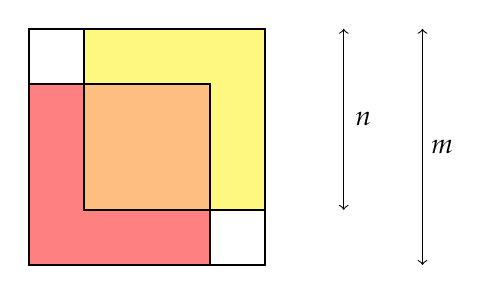
\begin{tikzpicture}
		\draw[thick] (0,0) rectangle (3,3);
		\draw[thick, fill=red!50] (0,0) rectangle (2.3,2.3);
		\draw[thick, fill=yellow!50] (0.7,0.7) rectangle (3, 3);
		\draw[thick, fill=orange!50] (0.7,0.7) rectangle (2.3, 2.3);
		\draw[<->] (4, 0.7)--(4, 3);
		\node at (4.25, 1.85) (n) {$n$};
		\draw[<->] (5, 0)--(5, 3);
		\node at (5.25, 1.5) (m) {$m$};
	\end{tikzpicture}
\end{center}
Puisque $m^2 = 2n^2$, la région où les deux carrés de côté $n$ se
recouvrent a la même aire que la région qu'aucun des deux ne couvre :
l'aire du carré orange est donc égale à la somme des aires des deux
carrés non colorés. Si le carré orange a pour côté $p$ et chacun des
carrés non colorés pour côté $q$, alors $p^2 = 2q^2$. Ainsi,
$\sqrt{2} = \nicefrac{p}{q}$, avec $p < m$, $q < n$ et $p, q \in
\Nat$.\footnote{Précision éditoriale : $p=2n-m$ et $q=m-n$. L'égalité $m^2=2n^2$, avec $m,n>0$, donne $n<m<2n$ ; ainsi $p,q>0$, $p<m$ et $q<n$. Les longueurs sont donc bien des naturels strictement positifs. Ces expressions des côtés sont explicites dans la présentation de Conway.}
Cela contredit la minimalité de $m$ et de $n$, assurée par le choix
d'une fraction irréductible.

\emph{Deuxièmement, par un raisonnement algébrique.} Comme
$m^{2} = 2n^{2}$, $m$ est pair. (On montre aisément que, si $x$ est
impair, alors $x^2$ est impair.) Il existe donc $r \in \Nat$ tel que
$m = 2r$. En réarrangeant, nous obtenons $2r^2 = n^2$,
		%\begin{align*}
		%	(2q)^{2} &= 2n^{2}\\
		%	4q^{2} &= 2n^{2}\\
		%	2q^{2} &= n^{2}
		%\end{align*}
et $n$ est donc lui aussi pair. Les deux nombres $m$ et $n$ étant
pairs, la fraction $\nicefrac{m}{n}$ \emph{peut} encore être simplifiée.
C'est une contradiction !{}
\end{proof}

Cette preuve par le dessin nous permet au passage de revenir à la
\olref[his][set][mythology]{sec}. Tennenbaum (1927--2006) était un
mathématicien tout à fait moderne ; pourtant, sa démonstration est
incontestablement élégante, parfaitement rigoureuse et fondée sur
l'intuition géométrique !{}

Quoi qu'il en soit, les réels forment un ensemble «~plus riche~» que les
rationnels. En un certain sens, les rationnels présentent des «~lacunes~»
que les réels comblent. Weierstrass a reconnu que cette idée s'exprime
par une propriété qui distingue les réels des rationnels : la
\emph{propriété de la borne supérieure}. Elle affirme que
\emph{tout ensemble non vide de nombres réels qui admet un majorant
admet un plus petit majorant.}

Il est facile de voir que les rationnels ne possèdent pas cette
propriété. Considérons par exemple l'ensemble des rationnels
strictement inférieurs à $\sqrt{2}$, c'est-à-dire :
\[
	\Setabs{p \in \Rat}{p^2 < 2 \text{ ou }p < 0}
\]
Cet ensemble admet un majorant rationnel : tous ses !!{element}s sont,
par exemple, strictement inférieurs à $3$. Mais quel serait son plus
petit majorant ? Nous voudrions répondre «~$\sqrt{2}$~» ; or nous venons
de voir que $\sqrt{2}$ n'est \emph{pas} rationnel. Et il n'existe pas
de \emph{plus petit} rationnel strictement supérieur à $\sqrt{2}$.
Cet ensemble admet donc un majorant rationnel, mais pas de plus petit
majorant rationnel. Les rationnels ne possèdent ainsi pas la propriété
de la borne supérieure.\footnote{Correction typographique : un signe $<$ parasite suivait le marqueur désignant les éléments dans la source. Il est retiré ; la comparaison avec $3$ reste inchangée.}

En revanche, la propriété de la borne supérieure répond à ce que nous
attendons intuitivement du continu. Nous ne voulons pas seulement que
$\sqrt{2}$ soit un nombre réel : nous voulons combler toutes les
«~lacunes~» de la droite rationnelle, et que le continu lui-même n'en
présente aucune. C'est précisément ce qu'assure cette propriété.


\endgroup
% END embedded source: content/sets-functions-relations/arithmetization/reals.tex


% BEGIN embedded source: content/sets-functions-relations/arithmetization/cuts.tex
\begingroup
\expandafter\def\csname ol@sectioncs\endcsname{section}
\def\olfilename{cuts}


\olfileid[fr]{sfr}{arith}{cuts}
\olsection{De $\Rat$ à $\Real$}

La propriété de la borne supérieure exprime, pour l'essentiel, la manière
dont un point $\alpha$ partage la droite réelle sans laisser de lacune :
il est la borne supérieure des points situés à sa gauche et la borne
inférieure de ceux situés à sa droite. Pour \emph{construire} les nombres
réels à partir des rationnels, Dedekind a proposé de prendre pour réels
les \emph{coupures} qui partagent les rationnels. Nous identifions ainsi
$\sqrt{2}$ à la \emph{coupure} qui sépare les rationnels
$< \sqrt{2}$ des rationnels $> \sqrt{2}$.

Précisons cette idée. Lorsque nous partageons les rationnels en deux
parties, la partie \emph{inférieure} suffit à déterminer la partition.
Nous adoptons donc la définition suivante :

\begin{defn}[Coupure]
Une \emph{coupure} $\alpha$ est un segment initial non vide et propre
de l'ensemble des rationnels, sans plus grand élément. Autrement dit,
$\alpha$ est une coupure si et seulement si :
\begin{enumerate}
	\item \emph{non vide et propre} : $\emptyset \neq \alpha \subsetneq \Rat$ ;
	\item \emph{segment initial} : pour tous $p,q \in \Rat$, si $p < q \in \alpha$, alors $p \in \alpha$ ;
	\item \emph{sans plus grand élément} : pour tout $p \in \alpha$, il existe $q \in \alpha$ tel que $p < q$.
\end{enumerate}
Nous définissons alors $\Real$ comme l'ensemble des coupures.
\end{defn}

Nous pouvons maintenant poser $\sqrt{2} = \Setabs{p \in \Rat}{p^2 < 2\text{
ou }p < 0}$. Bien entendu, il faut vérifier qu'il s'agit \emph{bien}
d'une coupure ; nous reportons cette vérification à la \olref[check]{sec}.

Comme précédemment, après avoir défini les objets, nous devons définir
les fonctions et relations usuelles sur leur ensemble. Commençons par
une relation simple :
\begin{align*}
	\alpha \leq \beta \liff \alpha \subseteq \beta.
\end{align*}
Cette définition de l'ordre permet d'\emph{énoncer} le résultat central :
l'ensemble des coupures possède la propriété de la borne supérieure.
Explicitons l'énoncé. Si $S$ est un ensemble non vide de coupures qui
admet un majorant, alors il admet un plus petit majorant. Plus précisément,
il existe une coupure $\lambda$ qui majore $S$, c'est-à-dire que
$(\forall \alpha \in S)\alpha \subseteq \lambda$, et $\lambda$ est la plus
petite de ces coupures, c'est-à-dire que
$(\forall \beta \in \Real)((\forall \alpha \in S)\alpha \subseteq \beta \lif \lambda \subseteq \beta)$.
Voici la démonstration :

\begin{thm}\ollabel{realcompleteness}
L'ensemble des coupures possède la propriété de la borne supérieure.
\end{thm}

\begin{proof}
Soit $S$ un ensemble non vide de coupures admettant un majorant. Posons
$\lambda = \bigcup S$.
%\Setabs{p \in \Rat}{(\exists \alpha \in S)p \in \alpha}$$
Montrons d'abord que $\lambda$ est une coupure :
\begin{enumerate}
\item Puisque $S$ est non vide, il contient au moins une coupure, elle-même
non vide ; ainsi $\emptyset \neq \lambda$.\footnote{Correction éditoriale : la source déduit à tort l'existence d'une coupure dans $S$ du fait que $S$ admet un majorant. C'est l'hypothèse $S\neq\emptyset$ qui intervient ici. La majoration est utilisée ensuite pour montrer que la réunion est propre.}
Puisque $S$ est un ensemble de coupures, $\lambda \subseteq \Rat$.
Comme $S$ admet une coupure majorante, un rationnel $p \in \Rat$
extérieur à cette coupure n'appartient à aucune coupure $\alpha \in S$.
Ainsi $p\notin \lambda$, donc $\lambda \subsetneq \Rat$.
\item Supposons que $p < q \in \lambda$. Il existe alors $\alpha \in S$
tel que $q \in \alpha$. Comme $\alpha$ est une coupure, $p \in \alpha$,
donc $p \in \lambda$.
\item Supposons que $p \in \lambda$. Il existe alors $\alpha \in S$
tel que $p \in \alpha$. Comme $\alpha$ est une coupure, il existe
$q \in \alpha$ tel que $p < q$. Nous avons donc aussi $q \in \lambda$.
\end{enumerate}
L'affirmation est démontrée. De plus,
$(\forall \alpha \in S)\alpha \subseteq \bigcup S = \lambda$ :
$\lambda$ est donc un majorant de $S$. Supposons maintenant que
$\beta \in \mathbb{R}$ soit un autre majorant, c'est-à-dire que
$(\forall \alpha \in S)\alpha \subseteq \beta$. Pour tout $p \in \Rat$,
si $p \in \lambda$, il existe $\alpha \in S$ tel que $p \in \alpha$,
et donc $p \in \beta$. Nous en déduisons $\lambda \subseteq \beta$.
Ainsi, $\lambda$ est le \emph{plus petit} majorant de $S$.
\end{proof}

Nous avons donc construit des objets qui satisfont la propriété de la
borne supérieure. Nous pouvons exprimer ce résultat en disant que nos
coupures ne présentent aucune «~lacune~» : former de nouvelles
«~coupures~» de réels, plutôt que de rationnels, ne fournirait pas
de nouveaux objets mathématiquement intéressants.

Définissons maintenant les opérations sur les réels. Commençons par
plonger les rationnels dans les réels en posant
$p_\Real = \Setabs{q \in \Rat}{q < p}$ pour chaque $p \in \Rat$.
Définissons ensuite :
\begin{align*}
	\alpha + \beta &= \Setabs{p + q}{p \in \alpha \land q \in \beta}\\
%	\alpha - \beta &\defis \Setabs{p - q}{p \in \alpha \land q \in \Rat \setminus \beta}\\
	\alpha \times \beta &=
	\Setabs{p \times q}{0 \leq p \in \alpha \land 0 \leq q \in \beta} \cup 0_\Real & \text{si }\alpha, \beta \geq 0_\Real.
%	\alpha \div \beta &\defis
%	\Setabs{\nicefrac{p}{q}}{p \in \alpha \land q \in \Rat \setminus \beta}  & \text{si }\alpha \geq 0_\Real, \beta > 0_\Real
\end{align*}
Pour traiter les autres cas du produit, posons d'abord
$0_\Real \times \alpha = 0_\Real = \alpha \times 0_\Real$ pour toute
coupure $\alpha$, puis définissons l'opposé :
% La source suggère en commentaire de poser d'abord l'annulation par la coupure nulle ; cette règle est rendue explicite ci-dessus.
\begin{align*}
	-\alpha &= \Setabs{p - q}{p,q \in \Rat \land p < 0 \land q \notin \alpha}.
\end{align*}
Posons enfin :
\begin{align*}
	\alpha \times \beta &\defis
	\begin{cases}
		\mathord{-}\alpha \times \mathord{-}\beta &\text{si }\alpha < 0_\Real\text{ et }\beta < 0_\Real\\
		\mathord{-}(\mathord{-}\alpha \times \beta) &\text{si }\alpha < 0_\Real \text{ et }\beta > 0_\Real\\
		\mathord{-}(\alpha \times \mathord{-}\beta) &\text{si }\alpha > 0_\Real \text{ et }\beta < 0_\Real.
	\end{cases}
\end{align*}
Il faut vérifier que chacune de ces définitions produit toujours une
coupure. Il restera enfin à établir, par une démonstration élémentaire
mais longue, que les coupures ainsi munies de ces opérations ont toutes
les propriétés attendues. Nous reportons ces vérifications à la
\olref[check]{sec}.\footnote{Corrections et précisions éditoriales : la notation $0^\mathbb{R}$ du produit positif est remplacée par $0_\Real$, la coupure nulle déjà définie. Les cas où un facteur est nul et l'autre strictement négatif manquaient dans les définitions actives ; la règle d'annulation, suggérée par un commentaire source, les complète. Dans la définition de l'opposé, les domaines rationnels de $p$ et $q$, implicites dans le contexte original, sont écrits explicitement.}

\endgroup
% END embedded source: content/sets-functions-relations/arithmetization/cuts.tex


% BEGIN embedded source: content/sets-functions-relations/arithmetization/reflections.tex
\begingroup
\expandafter\def\csname ol@sectioncs\endcsname{section}
\def\olfilename{reflections}


\olfileid[fr]{sfr}{arith}{ref}
\olsection{Quelques réflexions philosophiques}

Voilà pour les aspects techniques. Mais qu'avons-nous obtenu ?

D'abord, et cela ne prête guère à contestation, de très belles
mathématiques pures. Nous avons aussi obtenu des résultats conceptuels
profonds. Comprendre que la propriété de la borne supérieure exprime
la différence cruciale entre réels et rationnels constitue une avancée
majeure. De plus, la construction explicite des réels comme coupures de
Dedekind donne à l'analyse un fondement solide. Nous savons que la
notion de \emph{corps ordonné complet} est cohérente, puisque les
coupures forment précisément un tel corps.
\begin{editorial}
Cette dernière affirmation est relative au cadre ensembliste dans
lequel la construction est menée : celle-ci réalise les propriétés
d'un corps ordonné complet. Elle ne démontre pas, à elle seule,
la cohérence absolue de la théorie des ensembles employée.
\end{editorial}

Ces résultats appellent néanmoins quelques réserves.

Premièrement, il n'est pas clair qu'envisager les réels comme des
coupures soit \emph{plus} rigoureux que de les envisager à partir de
leurs développements décimaux familiers, éventuellement infinis.
Cette dernière « construction » ressemble quelque peu à celle par
les suites de Cauchy ; pour l'essentiel, elle était en fait connue
des mathématiciens dès le début du dix-septième siècle
(voir la \olref[cauchy]{sec}). Le véritable gain de rigueur est venu de
la reconnaissance de la propriété de la borne supérieure.
La possibilité de construire les réels comme des ensembles particuliers
n'est peut-être pas, à elle seule, si intéressante.

Il est encore moins clair que l'arithmétisation, beaucoup plus facile,
des entiers relatifs ou des rationnels accroisse la rigueur dans ces
domaines. Une observation simple mérite ici d'être faite. Après avoir
\emph{construit} les entiers relatifs comme classes d'équivalence de
couples ordonnés de naturels, puis les rationnels comme classes
d'équivalence de couples ordonnés d'entiers relatifs, puis les réels
comme ensembles de rationnels, nous \emph{oublions} immédiatement
ces constructions. En particulier, personne ne voudrait les
\emph{invoquer} dans une démonstration mathématique, sauf, bien sûr,
pour démontrer qu'elles ont les propriétés attendues. Il est bien
plus facile de parler directement d'un réel que d'un ensemble
d'ensembles d'ensembles d'ensembles d'ensembles d'ensembles d'ensembles
de naturels.
% (Les réels ont été construits comme ensembles de rationnels ;
% ceux-ci ont été construits comme classes d'équivalence de couples
% ordonnés d'entiers relatifs, c'est-à-dire comme ensembles d'ensembles
% d'ensembles d'entiers relatifs ; et ainsi de suite.)
% 2/3 = [2,3]
% c'est-à-dire {<2,3>, ... }
% { {{2},{2,3}}, ... }
%
% les réels sont
% des ensembles de rationnels
%
% les rationnels sont
% des ensembles d'ensembles d'ensembles d'entiers relatifs
%
% les entiers relatifs sont
% des ensembles d'ensembles d'ensembles de naturels

Plus douteux encore est que ces définitions nous disent ce que
\emph{sont} les entiers relatifs, les rationnels ou les réels,
\emph{sur le plan métaphysique}. Autrement dit, il est douteux que
les réels, par exemple, \emph{soient} certains ensembles
(d'ensembles d'ensembles\ldots). Le principal obstacle est que
la construction aurait pu être menée de bien des façons. Dans le
cas des réels, il existe des constructions différentes qui présentent
un réel intérêt (voir la \olref[cauchy]{sec}). Mais voici un moyen
tout à fait élémentaire d'obtenir d'autres constructions : comme
dans la \olref[sfr][rel][ref]{sec}, nous aurions pu définir les couples
ordonnés un peu autrement. Avec cette autre définition, nos
constructions auraient tout aussi bien fonctionné, mais nous aurions
obtenu d'autres objets. Il existe donc de nombreuses constructions
ensemblistes concurrentes des entiers relatifs, des rationnels et
des réels. Affirmer que les entiers relatifs, par exemple, sont
\emph{ces} ensembles plutôt que \emph{ceux-là} serait alors arbitraire,
et embarrassant. Comme dans la \olref[sfr][rel][ref]{sec}, il s'agit
d'un cas de l'argument rendu célèbre par \citealt{Benacerraf1965}.

Un autre point mérite d'être soulevé : nos constructions ont quelque
chose d'assez \emph{étrange}. Nous sommes partis des nombres naturels.
Nous construisons ensuite les entiers relatifs et le « $0$ des entiers
relatifs », c'est-à-dire $\equivrep{0,0}{\Intequiv}$.
Or, dans la réalisation ensembliste usuelle,
$0\neq\equivrep{0,0}{\Intequiv}$ ; avec ces constructions,
\emph{aucun} naturel n'est un entier relatif ainsi construit.
Cela paraît pourtant très contraire à l'intuition.
Dans la \olref[sfr][set][imp]{sec}, nous avons même affirmé,
sans véritable justification, que $\Nat\subseteq\Rat$.
Si ces constructions nous disent exactement \emph{ce que sont}
les nombres, cette affirmation, prise littéralement dans cette
réalisation, est manifestement fausse.
\begin{editorial}
Les inégalités et la séparation littérale invoquées ici dépendent du
codage des objets. Elles valent, par exemple, si les naturels sont les
ordinaux finis de von Neumann : les classes de couples qui représentent
les entiers relatifs et les rationnels sont infinies, tandis que chaque
naturel est un ensemble fini. La source laisse ce choix de réalisation
implicite. En revanche, les plongements déjà définis permettent
d'identifier chaque système de nombres à son image dans le suivant ;
ils justifient les inclusions usuelles après cette identification.
La distinction pertinente est celle entre égalité littérale des objets
et identification au moyen d'un plongement.
\end{editorial}

Prenons donc du recul. En travaillant dans une théorie naïve des
ensembles et en nous donnant les naturels, nous pouvons \emph{traiter}
les entiers relatifs, les rationnels et les réels comme certains
ensembles. En ce sens, nous pouvons \emph{plonger} les théories de
ces objets dans une théorie des ensembles. La portée philosophique
de ce plongement n'est cependant pas si simple à déterminer.

Bien sûr, ce n'est pas le dernier mot !{} Il s'agit seulement de
souligner ceci : montrer que l'arithmétisation des réels \emph{a}
une portée philosophique profonde exigerait un argument
\emph{philosophique} supplémentaire.

% De plus, tout au long de ce chapitre, nous avons tenu les naturels
% pour simplement donnés. Mais que pouvons-nous faire à leur sujet ?
% C'est l'objet du chapitre suivant.


\endgroup
% END embedded source: content/sets-functions-relations/arithmetization/reflections.tex


% BEGIN embedded source: content/sets-functions-relations/arithmetization/checking-details.tex
\begingroup
\expandafter\def\csname ol@sectioncs\endcsname{section}
\def\olfilename{checking-details}


\olfileid[fr]{sfr}{arith}{check}
\olsection{Anneaux et corps ordonnés}

Tout au long de ce chapitre, nous avons affirmé que certaines définitions
donnaient aux objets construits les propriétés « attendues ». Dans cette
annexe technique, nous allons préciser ce que nous entendons par là et
montrer, ou esquisser comment montrer, qu'elles ont bien cet effet.

Dans la \olref[int]{sec}, nous avons défini l'addition et la multiplication
sur $\Int$. Nous voulons montrer que ces opérations, telles que nous
les avons définies, munissent $\Int$ de la structure attendue.
Il s'agit, plus précisément, d'une structure d'anneau commutatif.

\Needspace{16\baselineskip}\begin{defn}
Un \emph{anneau commutatif} est un ensemble $S$ muni de deux éléments
distingués $0$ et $1$ et de deux opérations $+$ et $\times$ de
$S\times S$ dans $S$, qui satisfont les huit formules suivantes :
\begin{align*}
  \emph{Associativité}&&a + (b+ c) & = (a + b) + c \\
  && (a \times b) \times c & = a \times (b\times c)\\
  \emph{Commutativité}&&a + b &= b+ a  \\
  && a \times b&= b\times a\\
  \emph{Éléments neutres}&&a + 0 &= a \\
  && a \times 1 &= a\\
  \emph{Existence d'un opposé}&&(\exists b\in S)0&=a + b\\
  \emph{Distributivité}&&a \times (b+ c ) &= (a \times b) + (a \times c)
\end{align*}
Dans chaque formule, les variables libres sont implicitement quantifiées
universellement sur $S$ ; le $b$ de la formule sur l'opposé est déjà lié
par son quantificateur existentiel. Les éléments $0$ et~$1$ ne sont pas
nécessairement les nombres naturels qui portent ces noms.
\end{defn}

Pour vérifier que les entiers relatifs forment un anneau commutatif, il
suffit donc de vérifier ces huit conditions. Aucune n'est difficile à
établir, mais l'ensemble des vérifications est un peu laborieux. Voici,
par exemple, comment démontrer l'\emph{associativité} de l'addition :

\begin{proof}
Fixons $i, j, k \in \Int$. Il existe donc
$a_1, b_1, a_2, b_2, a_3, b_3 \in \Nat$ tels que
$i = \equivrep{a_1, b_1}{}$, $j = \equivrep{a_2,b_2}{}$ et
$k = \equivrep{a_3, b_3}{}$. Pour alléger les notations, nous écrivons
« $\equivrep{x, y}{}$ » au lieu de
« $\equivrep{x, y}{\Intequiv}$ » dans toute cette section. On a alors :
\begin{align*}
  i + (j + k) &= \equivrep{a_1, b_1}{}+(\equivrep{a_2, b_2}{} + \equivrep{a_3, b_3}{}) \\
  &= \equivrep{a_1, b_1}{} + \equivrep{a_2+a_3, b_2+b_3}{}\\
  &= \equivrep{a_1 + (a_2 + a_3), b_1 + (b_2 + b_3)}{}\\
  &= \equivrep{(a_1 + a_2) + a_3, (b_1 + b_2) + b_3}{}\\
  &= \equivrep{a_1 + a_2, b_1 + b_2}{} + \equivrep{a_3, b_3}{}\\
  &= (\equivrep{a_1, b_1}{} + \equivrep{a_2, b_2}{}) + \equivrep{a_3, b_3}{}\\
  &= (i+j) + k
\end{align*}
en utilisant librement les propriétés de l'addition dans $\Nat$.
\end{proof}

De même, voici comment établir l'\emph{existence d'un opposé} :

\begin{proof}
Fixons $i \in \Int$ ; on a donc $i = \equivrep{a,b}{}$ pour certains
$a,b \in \Nat$. Posons $j = \equivrep{b,a}{} \in \Int$.
Les propriétés des naturels donnent $(a+b) + 0 = 0 + (a+b)$.
Par définition, $\tuple{a+b, b+a} \sim_\Int \tuple{0,0}$, d'où
$\equivrep{a+b, b+a}{} = \equivrep{0, 0}{} = 0_\Int$.
Ainsi, $i + j = \equivrep{a,b}{}+\equivrep{b,a}{}
=\equivrep{a+b, b+a}{}=\equivrep{0,0}{} = 0_\Int$.
\end{proof}

Voici enfin une démonstration de la \emph{distributivité} :

\begin{proof}
Comme ci-dessus, fixons $i = \equivrep{a_1, b_1}{}$,
$j = \equivrep{a_2,b_2}{}$ et $k = \equivrep{a_3, b_3}{}$. Alors :
\begin{align*}
  i \times (j + k)
  &= \equivrep{a_1, b_1}{} \times (\equivrep{a_2,b_2}{} + \equivrep{a_3, b_3}{})\\
  &= \equivrep{a_1, b_1}{} \times \equivrep{a_2 + a_3,b_2+b_3}{}\\
  &= \equivrep{a_1 (a_2 + a_3) + b_1 (b_2+b_3), a_1 (b_2 + b_3) + b_1 (a_2 + a_3)}{}\\
  &= \equivrep{a_1 a_2 + a_1a_3 + b_1 b_2+b_1b_3, a_1 b_2 + a_1b_3 + a_2b_1 + a_3b_1}{}\\
% Ligne inactive de la source, erronée par répétition du terme b_1b_2 :
% &= \equivrep{a_1 a_2 + b_1b_2 + a_1a_3 + b_1 b_2+b_1b_3, a_1 b_2 + a_1b_3 + a_2b_1 + a_3b_1}{}\\
  &= \equivrep{a_1a_2 + b_1b_2, a_1b_2 + a_2b_1}{} + \equivrep{a_1a_3 + b_1b_3, a_1b_3 + a_3b_1}{}\\
  &= (\equivrep{a_1, b_1}{} \times \equivrep{a_2,b_2}{}) + (\equivrep{a_1, b_1}{} \times \equivrep{a_3, b_3}{})\\
  &= (i \times j) + (i \times k)
\end{align*}
\end{proof}

Nous laissons en exercice la démonstration des cinq autres conditions.
Une fois ces vérifications faites, nous aurons montré que $\Int$ forme
un anneau commutatif : l'addition et la multiplication définies plus
haut ont bien les propriétés attendues.

\begin{prob}
Démontrer que $\Int$ est un anneau commutatif.
\end{prob}

Le travail n'est toutefois pas terminé. Outre l'addition et la
multiplication sur $\Int$, nous avons défini une relation d'ordre
$\leq$ ; il faut vérifier qu'elle aussi a les propriétés attendues.
Plus précisément, il faut montrer que $\Int$ est un anneau
\emph{ordonné}.\footnote{Rappelons, d'après la
\olref[sfr][rel][ord]{def:linearorder}, qu'un ordre total est une
relation réflexive, transitive, antisymétrique et connexe. Pour un tel
ordre, la connexité donne la \emph{trichotomie} de l'ordre strict
associé : pour tous $a$ et $b$, exactement l'une des relations
$a < b$, $a = b$, $a > b$ est vérifiée.
\emph{Précision éditoriale :} la source écrit ici
$a \leq b \lor a = b \lor a \geq b$ ; cette disjonction est vraie,
mais ses trois cas ne sont pas exclusifs.}

\begin{defn}
Un \emph{anneau ordonné} est un anneau commutatif muni d'une relation
d'ordre total $\leq$ telle que, pour tous $a,b,c\in S$ :
\begin{align*}
  a \leq b &\lif a + c \leq b + c\\
  (a \leq b \land 0 \leq c) &\lif a \times c \leq b \times c
\end{align*}
\end{defn}

\begin{prob}
Démontrer que $\Int$ est un anneau ordonné.
\end{prob}

Comme précédemment, montrer que $\Int$, tel que nous l'avons construit,
est un anneau ordonné demande des vérifications laborieuses mais
usuelles. Nous vous les laissons.

Cela règle le cas des entiers relatifs. Il faut maintenant établir des
propriétés très semblables pour les rationnels. Plus précisément, nous
devons montrer qu'avec nos définitions de $+$, $\times$ et $\leq$, les
rationnels forment un \emph{corps} ordonné :
\begin{defn}\ollabel{orderedfield}
Un \emph{corps ordonné} est un anneau ordonné $S$ dans lequel
$0\neq1$ et qui satisfait en outre :
\begin{align*}
  \emph{Existence d'un inverse}& &
  (\forall a \in S \setminus \{0\})(\exists b \in S) a\times b& = 1
\end{align*}
\end{defn}
\begin{editorial}
La condition $0\neq1$, omise dans la source, exclut l'anneau réduit à un
seul élément. Sans elle, la condition sur les éléments non nuls serait
vide et ne suffirait pas à définir un corps.
\end{editorial}

Une fois établi que $\Int$ est un anneau ordonné, il est facile, quoique
laborieux, de montrer que $\Rat$ est un corps ordonné.

\begin{prob}
Démontrer que $\Rat$ est un corps ordonné.
\end{prob}

Après les entiers relatifs et les rationnels, il ne reste que les réels.
Il faut montrer que $\Real$ est un corps ordonné \emph{complet},
c'est-à-dire un corps ordonné ayant la propriété de la borne supérieure.
Or, le \olref[cuts]{realcompleteness} établit déjà cette propriété pour
$\Real$. Il reste toutefois à effectuer les vérifications, fastidieuses,
qui montrent que $\Real$ est un corps ordonné.

Avant d'entreprendre cet exercice laborieux, il faut vérifier quelques
faits plus « immédiats ». Par exemple, nous devons nous assurer que
$\alpha + \beta$, tel que nous l'avons défini, est bien une
\emph{coupure} dès que $\alpha$ et $\beta$ sont des coupures.
En voici une démonstration :

\begin{proof}
Puisque $\alpha$ et $\beta$ sont des coupures,
$\alpha + \beta = \Setabs{p + q}{p \in \alpha \land q \in \beta}$
est une partie non vide et propre de $\Rat$. En effet, chacune des
deux coupures contient un rationnel, dont la somme appartient à
$\alpha+\beta$. Choisissons aussi $r\in\Rat\setminus\alpha$ et
$s\in\Rat\setminus\beta$. Tout $p\in\alpha$ vérifie $p<r$ et tout
$q\in\beta$ vérifie $q<s$, car les coupures sont des segments initiaux.
Ainsi $p+q<r+s$, et $r+s\notin\alpha+\beta$.
Supposons maintenant que $x < p + q$ pour certains $p \in \alpha$ et
$q \in \beta$, avec $x\in\Rat$. Alors $x - p < q$, donc
$x - p \in \beta$, et $x = p + (x - p) \in \alpha + \beta$.
La somme est donc un segment initial de $\Rat$.
Enfin, pour tout $p + q \in \alpha + \beta$, les deux coupures étant
sans maximum, il existe $p_1 \in \alpha$ et $q_1 \in \beta$ tels que
$p < p_1$ et $q < q_1$. Ainsi
$p + q < p_1 + q_1 \in \alpha + \beta$, et $\alpha+\beta$ n'a pas de maximum.
\end{proof}

Des vérifications analogues permettent de montrer que $\alpha - \beta$,
$\alpha \times \beta$ et $\alpha \div \beta$ sont des coupures, en
excluant, dans le dernier cas, celui où $\beta$ est la coupure nulle.
Là encore, nous vous laissons ces vérifications.
\begin{editorial}
La source n'active pas ses définitions de la soustraction et de la
division des coupures. Pour donner un sens précis à cet exercice,
on pose $\alpha-\beta=\alpha+(-\beta)$ et
$\alpha\div\beta=\alpha\times\beta^{-1}$ pour $\beta\neq0_\Real$.
Si $\beta>0_\Real$, on définit
\[
\beta^{-1}=\Setabs{q\in\Rat}{q\leq0\ \lor\
(\exists r\in\Rat\setminus\beta)(r>0\land q<1/r)}.
\]
Si $\beta<0_\Real$, on pose $\beta^{-1}=-((-\beta)^{-1})$.
Les opposés et les produits sont ceux définis précédemment ; vérifier
que cette construction donne bien l'inverse fait partie de l'exercice.
\end{editorial}

\begin{prob}
Démontrer que $\Real$ est un corps ordonné.
\end{prob}

Il reste enfin un petit point à régler. Dans la \olref[cuts]{sec},
nous proposons de prendre
$\sqrt{2}=\Setabs{p \in \Rat}{p < 0 \text{ ou }p^2 < 2}$.
Il faut cependant montrer que cet ensemble est une \emph{coupure}.
En voici une démonstration :

\begin{proof}
Cet ensemble est un segment initial non vide et propre de $\Rat$ :
il contient $1$ et ne contient pas $2$ ; si $x<p$ et si $p$ appartient
à l'ensemble, alors soit $x<0$, soit $0\leq x<p$ et $x^2<p^2<2$.
Il suffit donc de montrer qu'il n'a pas de maximum. Si $p\leq0$,
l'élément $1$ lui est supérieur. Il suffit ainsi de traiter le cas
d'un rationnel strictement positif $p$ tel que $p^2<2$.
Posons $q=\frac{2p+2}{p+2}$ et montrons que $p<q$ et $q^2<2$.
Puisque $p+2>0$, la première inégalité résulte du calcul suivant :
\begin{align*}
  p^2 &< 2\\
  p^2 + 2p &< 2 + 2p\\
  p(p + 2) &< 2 + 2p\\
  p &< \tfrac{2+2p}{p+2} = q
\end{align*}
Pour établir $q^2<2$, il suffit de remarquer que :
\begin{align*}
  p^2 &< 2\\
  2p^2 + 4p + 2 &< p^2 + 4p+ 4\\
  4p^2 + 8p + 4 &< 2(p^2 + 4p + 4)\\
  (2p+2)^2 &< 2(p+2)^2\\
  \tfrac{(2p+2)^2}{(p+2)^2} &< 2\\
  q^2 &< 2
\end{align*}
\end{proof}

\endgroup
% END embedded source: content/sets-functions-relations/arithmetization/checking-details.tex


% BEGIN embedded source: content/sets-functions-relations/arithmetization/cauchy.tex
\begingroup
\expandafter\def\csname ol@sectioncs\endcsname{section}
\def\olfilename{cauchy}


\olfileid[fr]{sfr}{arith}{cauchy}

\olsection{Annexe : les réels construits à partir des suites de Cauchy}

Dans la \olref[cuts]{sec}, nous avons construit les réels comme coupures
de Dedekind. Nous allons présenter ici une autre construction. Elle
s'appuie sur la définition, due à Cauchy, de ce que nous appelons
aujourd'hui une suite de Cauchy. Son emploi pour \emph{construire} les
réels est toutefois dû à d'autres auteurs du dix-neuvième siècle,
notamment Weierstrass, Heine, M\'{e}ray et Cantor. Pour un exposé
historique, voir \citeauthor{OConnorRobertson:RN}
\citeyear{OConnorRobertson:RN}.

Avant d'aborder le dix-neuvième siècle, arrêtons-nous sur Simon Stevin
(1548--1620). Pour résumer, Stevin a compris que l'on pouvait envisager
chaque réel à partir de son développement décimal. Même un nombre
irrationnel tel que $\sqrt{2}$ possède un développement décimal dont
le début est :
\[
1{,}41421356237\ldots
\]
Il est très facile de représenter ces développements en théorie des
ensembles : il suffit de les considérer comme des fonctions
$d \colon \Nat \to \Nat$, où $d(n)$ est le chiffre décimal de rang $n$
qui nous intéresse. Il faut ensuite adapter un peu cette représentation
pour tenir compte de ce qui précède la virgule, ici simplement $1$.
Une autre adaptation, au moyen d'une relation d'équivalence, garantit
par exemple que $0{,}999\ldots=1$. Il n'est cependant pas difficile de
donner, dans l'esprit de Stevin, une construction parfaitement rigoureuse
des réels en théorie des ensembles.
\begin{editorial}
Les valeurs de $d$ sont des chiffres : elles doivent donc appartenir à
$\{0,\ldots,9\}$, restriction laissée implicite dans la source. Pour
représenter tous les réels, il faut également coder le signe et la partie
entière, puis identifier les deux écritures éventuelles d'un même nombre.
\end{editorial}

Stevin ne sera pas notre sujet principal ; pour en savoir davantage,
voir \citealt{KatzKatz2012}. Considérons plutôt une idée très proche.
Au lieu de traiter directement le développement décimal de $\sqrt{2}$,
on peut considérer une \emph{suite} d'approximations rationnelles de
plus en plus précises, obtenues en conservant davantage de chiffres :
\[
1;\ 1{,}4;\ 1{,}414;\ 1{,}4142;\ 1{,}41421;\ldots
\]
L'idée de représenter les réels par des « approximations de plus en
plus précises » conduit à une nouvelle série d'observations, analogues
à celles qui ont guidé la construction de $\Rat$ à partir de $\Int$,
ou de $\Int$ à partir de $\Nat$ :
\begin{enumerate}
\item Tout réel admet un développement décimal, éventuellement infini.
\item L'information contenue dans un tel développement peut tout aussi
bien être représentée par une suite de nombres rationnels.
\item Une suite de rationnels peut être considérée comme une fonction
de $\Nat$ dans $\Rat$ : il suffit de prendre pour $f(n)$ le rationnel
de rang $n$ de la suite.
\end{enumerate}
Bien entendu, une fonction \emph{quelconque} de $\Nat$ dans $\Rat$
ne nous donne pas nécessairement un réel. Considérons par exemple :
\[
f(n)=\begin{cases}
1 &\text{si }n\text{ est impair}\\
0 &\text{si }n\text{ est pair}
\end{cases}
\]
La difficulté est que la suite $0,1,0,1,0,1,0,\ldots$ ne semble
« se rapprocher » d'aucun réel. Pour retenir des suites qui se rapprochent
effectivement d'un réel, il faut donc une condition correspondant à
l'existence d'une \emph{limite}.

Nous avons déjà rencontré la notion de limite dans la
\olref[his][set][limits]{sec}. Nous ne pouvons pourtant pas reprendre
exactement la même définition. L'expression « $(\forall\epsilon>0)$ »
y quantifiait implicitement sur les réels, et nous considérions des
limites de fonctions définies sur les réels. Invoquer cette définition
supposerait donc déjà les réels, alors que nous cherchons précisément
à les \emph{construire}. Heureusement, une notion étroitement liée à
celle de limite permet de procéder autrement.
\begin{defn}\ollabel{def:CauchySequence}
Une fonction $f:\Nat\to\Rat$ est une \emph{suite de Cauchy} si et
seulement si, pour tout $\epsilon\in\Rat$ strictement positif,
$(\exists\ell\in\Nat)(\forall m,n>\ell)|f(m)-f(n)|<\epsilon$,
où $m$ et $n$ parcourent les naturels.
\end{defn}

L'idée reste celle d'une précision prescrite : pour un degré de
précision mesuré par $\epsilon$, on trouve un rang $\ell$ au-delà
duquel les termes sont suffisamment proches les uns des autres.
Notre suite $1$, $1{,}4$, $1{,}414$, $1{,}4142$, $1{,}41421$\ldots
illustre cette idée : pour approcher $\sqrt{2}$ avec une erreur
inférieure à $\nicefrac{1}{10^n}$, il suffit de considérer les termes
situés après celui de rang $n$.
\begin{editorial}
Le langage de la limite réelle reste ici une motivation intuitive,
ou renvoie au réel déjà construit par coupures. La définition de
Cauchy n'affirme pas qu'une limite existe dans $\Rat$ : elle compare
deux termes de la suite. Pour obtenir la condition de Cauchy à partir
d'approximations d'erreur donnée, on prend chaque erreur inférieure à
$\epsilon/2$ et on applique l'inégalité triangulaire.
\end{editorial}

On pourrait alors être tenté de dire qu'un réel \emph{est} simplement
une suite de Cauchy. Ce serait toutefois trop naïf, comme dans les
constructions de $\Int$ et de $\Rat$ : plusieurs suites de Cauchy
distinctes peuvent représenter le même réel. Pour le voir, prenons une
suite de Cauchy $f$ et définissons $g$ exactement comme $f$, sauf que
$g(0)\neq f(0)$. Les deux suites coïncident après le premier terme.
Le critère de la \olref{def:CauchySequence} est donc satisfait par l'une
comme par l'autre, et nous voudrons, au terme de la construction, leur
attribuer la même limite. Elles doivent ainsi « définir » le même réel
et être identifiées en tant que représentations de ce réel.

Il nous faut donc, une nouvelle fois, définir une relation d'équivalence
sur les suites de Cauchy et identifier les réels à des classes
d'équivalence. Définissons d'abord ce que signifie tendre vers $0$.
Pour une fonction $h:\Nat\to\Rat$, on dit que \emph{$h$ tend vers $0$}
si et seulement si, pour tout $\epsilon\in\Rat$ strictement positif,
$(\exists\ell\in\Nat)(\forall n>\ell)|h(n)|<\epsilon$, où $n\in\Nat$.
\footnote{Comparer avec la définition de
$\lim_{x\mathord{\rightarrow}\infty}f(x)=0$ dans la
\olref[his][set][limits]{sec}.}
Pour deux fonctions $f,g:\Nat\to\Rat$, posons en outre
$(f-g)(n)=f(n)-g(n)$. Définissons alors :
\[
f\Realequiv g\quad\text{si et seulement si }(f-g)\text{ tend vers }0.
\]
Il faut vérifier que $\Realequiv$ est une relation d'équivalence ;
c'est bien le cas. On peut alors définir les réels comme les classes,
pour $\Realequiv$, de toutes les suites de Cauchy de $\Nat$ dans $\Rat$.
\begin{editorial}
La source écrit d'abord « relations d'équivalence » là où il faut
« classes d'équivalence ». De même, ce sont les classes de suites qui
formeront un corps ordonné dans les énoncés qui suivent. Une suite
représentante et sa classe sont désormais distinguées partout.
\end{editorial}

\begin{prob}
Posons $f(n)=0$ pour tout $n$ et $g(n)=\frac{1}{(n+1)^2}$.
Montrer que ce sont deux suites de Cauchy et, plus précisément, que
toutes deux tendent vers $0$, de sorte que $f\sim_\Real g$.
\end{prob}

Comme d'habitude, nous noterons $\equivrep{f}{\Realequiv}$ la classe
d'équivalence ayant $f$ pour !!a{element}. Pour alléger la lecture,
nous omettrons désormais l'indice et écrirons simplement
$\equivrep{f}{}$. Pour tout $q\in\Rat$, nous posons aussi
$q_\Real=\equivrep{c_q}{}$, où $c_q$ est la fonction constante définie
par $c_q(n)=q$ pour tout $n\in\Nat$. Nous définissons alors les
relations et les opérations de base sur les réels, par exemple :
\begin{align*}
\equivrep{f}{}+\equivrep{g}{}&=\equivrep{(f+g)}{}\\
\equivrep{f}{}\times\equivrep{g}{}&=\equivrep{(f\times g)}{}
\end{align*}
où $(f+g)(n)=f(n)+g(n)$ et $(f\times g)(n)=f(n)\times g(n)$.
Il faut bien sûr vérifier que $(f+g)$, $(f-g)$ et $(f\times g)$ sont
des suites de Cauchy lorsque $f$ et $g$ en sont ; c'est effectivement
le cas, et nous vous laissons cette vérification.
\begin{editorial}
Il faut également vérifier que les opérations sur les classes ne
dépendent pas des représentants choisis. La stabilité des suites de
Cauchy sous les opérations ne suffit pas, à elle seule, à l'établir.
\end{editorial}

Définissons enfin l'ordre. La classe $\equivrep{f}{}$ est
\emph{strictement positive} si et seulement si
$\equivrep{f}{}\neq0_\Real$ et
$(\exists\ell\in\Nat)(\forall n>\ell)0<f(n)$.
On pose $\equivrep{f}{}<\equivrep{g}{}$ si et seulement si
$\equivrep{(g-f)}{}$ est strictement positive. Il faut vérifier que
cette définition ne dépend pas du choix de la fonction représentante
dans chaque classe d'équivalence.
% Variante inactive conservée de la source. Le cas d'égalité des classes
% est nécessaire : l'inégalité large terme à terme, seule, ne descend
% pas au quotient.
%\begin{align*}
%\equivrep{f}{}\leq\equivrep{g}{}\text{ ssi }&\equivrep{f}{}=\equivrep{g}{}\text{ ou }\\
%&( \exists \ell\in\Nat)(\forall n\in\Nat)(\ell<n\lif f(n)\leq g(n))
%\end{align*}
Une fois cette vérification faite, les propriétés algébriques attendues
s'établissent assez facilement. Autrement dit :
\begin{editorial}
Nous avons corrigé $0_\Rat$ en $0_\Real$ dans la définition de
positivité. La condition que la classe soit non nulle est essentielle :
une suite peut être strictement positive à chaque rang et tendre vers
zéro. Pour justifier l'ordre et les inverses, on utilise le fait
suivant : si une suite de Cauchy $u$ ne tend pas vers zéro, il existe
un rationnel $\delta>0$ tel qu'à partir d'un certain rang,
$|u(n)|>\delta$ et tous les $u(n)$ ont le même signe. En effet, il
existe $\epsilon_0>0$ rationnel tel que des termes arbitrairement
tardifs aient une valeur absolue au moins égale à $\epsilon_0$.
Au-delà d'un rang où les écarts entre termes sont inférieurs à
$\epsilon_0/2$, tous les termes sont donc du même signe et de valeur
absolue supérieure à $\epsilon_0/2$. Ce fait montre aussi que le signe
de la classe ne change pas lorsqu'on remplace $u$ par une suite
équivalente. Pour une classe non nulle, on peut prendre comme
représentante de l'inverse la suite égale à $1/u(n)$ à partir de ce
rang, et à $1$ avant celui-ci. La vérification qu'elle est de Cauchy
utilise
$|1/u(m)-1/u(n)|\leq |u(m)-u(n)|/\delta^2$.
\end{editorial}
\begin{thm}\ollabel{thm:cauchyorderedfield}
Les classes d'équivalence de suites de Cauchy forment un corps ordonné.
\end{thm}

\begin{proof}
En exercice.
\end{proof}

\begin{prob}
Démontrer que les classes d'équivalence de suites de Cauchy forment
un corps ordonné.
\end{prob}

La propriété de la borne supérieure est plus difficile à établir pour
les réels ainsi construits ; nous allons donc en donner la démonstration.

\begin{thm}
Tout ensemble non vide et majoré de classes d'équivalence de suites
de Cauchy admet une borne supérieure.
\end{thm}

\begin{proof}[Esquisse de démonstration]
Soit $\mathcal A$ un ensemble non vide et majoré de classes de suites
de Cauchy. Pour conserver les notations de la construction ci-dessous,
notons $S$ l'ensemble de toutes les suites $h$ telles que
$\equivrep{h}{}\in\mathcal A$. Les éléments de $S$ sont donc des suites,
et ceux de $\mathcal A$ des classes. Il existe $p\in\Rat$ tel que
$p_\Real$ majore $\mathcal A$. Choisissons $r\in S$ ; il existe
$q\in\Rat$ tel que $q_\Real<\equivrep{r}{}$. Ces bornes rationnelles
existent parce que toute suite de Cauchy rationnelle est bornée :
on applique cette observation à une représentante d'un majorant
de $\mathcal A$, puis à $r$. Si la borne supérieure de $\mathcal A$
existe, elle se trouve donc entre $q_\Real$ et $p_\Real$, bornes comprises.

Nous allons nous rapprocher de cette borne supérieure simultanément
par valeurs inférieures et supérieures. Définissons deux fonctions
$f,g:\Nat\to\Rat$, destinées à l'approcher respectivement par valeurs
supérieures et inférieures. Posons d'abord :
\begin{align*}
f(0)&=p\\
g(0)&=q
\end{align*}
Puis, en posant $a_n=\frac{f(n)+g(n)}2$, définissons :
\footnote{Il s'agit d'une définition par récurrence. Nous n'avons
cependant pas encore justifié l'emploi de telles définitions.}
\begin{align*}
f(n+1)&=\begin{cases}
a_n &\text{si }(\forall h\in S)\equivrep{h}{}\leq(a_n)_\Real\\
f(n)&\text{sinon}
\end{cases}\\
g(n+1)&=\begin{cases}
a_n &\text{si }(\exists h\in S)\equivrep{h}{}\geq(a_n)_\Real\\
g(n)&\text{sinon}
\end{cases}
\end{align*}
Les suites $f$ et $g$ sont de Cauchy. On peut le vérifier assez
facilement ; nous laissons le détail de cette vérification en exercice.
Voici les observations utiles : $f$ est décroissante, $g$ est
croissante, les intervalles $[g(n),f(n)]$ sont emboîtés et
\[
0\leq f(n+1)-g(n+1)\leq\frac{f(n)-g(n)}2.
\]
Leur longueur est donc au plus $(p-q)/2^n$. Deux termes suffisamment
tardifs de l'une ou l'autre suite appartiennent au même intervalle,
aussi petit que voulu. En particulier, $(f-g)$ tend vers $0$,
d'où $\equivrep{f}{}=\equivrep{g}{}$.
\emph{Précision éditoriale :} la source affirme que l'écart est divisé
exactement par deux à chaque étape. Avec ses deux conditions larges,
les deux premières branches peuvent s'appliquer simultanément, lorsque
le milieu est un maximum de $\mathcal A$ ; l'écart devient alors nul.
L'inégalité ci-dessus couvre aussi ce cas. Par construction, pour
chaque $n$, $(f(n))_\Real$ majore $\mathcal A$, et il existe
$h\in S$ tel que $(g(n))_\Real\leq\equivrep{h}{}$.

Montrons d'abord que $\equivrep{f}{}$ majore $\mathcal A$,
c'est-à-dire que
$(\forall h\in S)\equivrep{h}{}\leq\equivrep{f}{}$.
Nous utiliserons le \olref{thm:cauchyorderedfield} au cours du raisonnement.
Soit $h\in S$ et supposons, pour obtenir une contradiction, que
$\equivrep{f}{}<\equivrep{h}{}$, donc que
$0_\Real<\equivrep{(h-f)}{}$. La suite $f$ étant de Cauchy et
décroissante, il existe $n\in\Nat$ tel que
$\equivrep{(c_{f(n)}-f)}{}<\equivrep{(h-f)}{}$.
En effet, la positivité de la classe de $h-f$ donne un écart rationnel
$\delta>0$ tel que $h(m)-f(m)>\delta$ à partir d'un certain rang ;
on choisit $n$ assez grand pour que, pour tout $m$ assez grand,
$|f(n)-f(m)|<\delta/2$. La suite
$(h-f)-(c_{f(n)}-f)$ est alors, à partir d'un certain rang,
strictement supérieure à $\delta/2$.
Ainsi :
\[
(f(n))_\Real=\equivrep{c_{f(n)}}{}
<\equivrep{f}{}+\equivrep{(h-f)}{}=\equivrep{h}{},
\]
ce qui contredit $\equivrep{h}{}\leq(f(n))_\Real$, vraie par construction.

Montrons enfin que $\equivrep{f}{}=\equivrep{g}{}$ est le
\emph{plus petit} majorant de $\mathcal A$. Soit $j$ une suite de
Cauchy telle que $\equivrep{j}{}<\equivrep{g}{}$.
Comme ci-dessus, en utilisant cette fois la croissance de $g$,
il existe $n\in\Nat$ tel que $\equivrep{j}{}<(g(n))_\Real$ :
on prend un écart strictement positif pour $g-j$, puis un rang
où les écarts entre termes de $g$ lui sont inférieurs de moitié.
Or, par construction, il existe $h\in S$ tel que
$(g(n))_\Real\leq\equivrep{h}{}$. On a donc
$\equivrep{j}{}<\equivrep{h}{}$, et $\equivrep{j}{}$ ne majore pas
$\mathcal A$.
\end{proof}


\endgroup
% END embedded source: content/sets-functions-relations/arithmetization/cauchy.tex


\OLEndChapterHook


\endgroup
% END embedded source: content/sets-functions-relations/arithmetization/arithmetization.tex


% BEGIN embedded source: content/sets-functions-relations/infinite/infinite.tex
\begingroup
\expandafter\def\csname ol@sectioncs\endcsname{section}
\def\olfilename{infinite}


\olchapter{sfr}{infinite}{Ensembles infinis}

\begin{editorial}
Ce chapitre consacré aux ensembles infinis est tiré de
\emph{Open Set Theory}, de Tim Button.
\end{editorial}


% BEGIN embedded source: content/sets-functions-relations/infinite/hilberts-hotel.tex
\begingroup
\expandafter\def\csname ol@sectioncs\endcsname{section}
\def\olfilename{hilberts-hotel}


\olfileid[fr]{sfr}{infinite}{hilbert}
\olsection{L'hôtel de Hilbert}

L'ensemble des entiers naturels est manifestement infini. Aussi, si nous
ne voulons pas \emph{supposer d'emblée l'existence} des entiers naturels,
notre première étape doit consister à caractériser un ensemble infini
dans des termes qui ne nécessitent pas de mentionner les entiers naturels
eux-mêmes. Voici une approche intéressante, présentée par Hilbert dans
ses cours de l'hiver 1924--1925.\footnote{Note de l'édition française :
la source indique 1924. Nous précisons ici l'intervalle du semestre
d'hiver 1924--1925 donné par les éditeurs pour ces cours, sans attribuer
une date précise à cette séance.} Il nous demande d'imaginer
\begin{quote}
[\ldots] un hôtel ayant un nombre fini de chambres. Toutes ces chambres
doivent être occupées par exactement un client. Si les clients échangent
maintenant leurs chambres d'une manière quelconque, [mais] de telle sorte
que chaque chambre contienne encore au plus une personne, aucune chambre
ne se libérera, et le propriétaire de l'hôtel ne pourra pas créer ainsi
une place pour un client qui vient d'arriver [\ldots
\textparagraph \ldots]

Supposons maintenant que l'hôtel possède une infinité de chambres
numérotées $1$, $2$, $3$, $4$, $5$, \dots, chacune occupée par exactement
un client. Dès qu'un nouveau client arrive, il suffit au propriétaire
de déplacer chacun des clients déjà présents dans la chambre dont le
numéro est supérieur d'une unité, et la chambre~$1$ sera libre pour le
client qui vient d'arriver.
	\begin{center}
		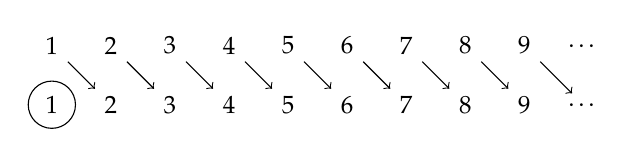
\begin{tikzpicture}[scale = .75]
		\foreach \x in {1, 2, 3, 4, 5, 6, 7, 8, 9}
		{
			\node (\x a) at (\x, 1) {\small{\x}};
			\node (\x b) at (\x, 2) {\small{\x}};
		}
		\node (dotsa) at (10, 1) {\small{\ldots}};
		\node (dotsb) at (10, 2) {\small{\ldots}};
		\draw[->] (1b)--(2a);
		\draw[->] (2b)--(3a);
		\draw[->] (3b)--(4a);
		\draw[->] (4b)--(5a);
		\draw[->] (5b)--(6a);
		\draw[->] (6b)--(7a);
		\draw[->] (7b)--(8a);
		\draw[->] (8b)--(9a);
		\draw[->] (9b)--(dotsa);
		\draw (1,1) circle (.4);
		\end{tikzpicture}
	\end{center}
	(publié dans \citealt[730]{EwaldSieg2013} ; traduction française
	d'après la traduction anglaise donnée dans la source)
\end{quote}
Le point crucial est que l'hôtel de Hilbert possède une infinité de
chambres ; nous pouvons prendre cette explication pour définir ce que
cela signifie. C'était précisément l'approche de Dedekind, présentée
ici, bien entendu, au prix d'un anachronisme considérable : sa définition
date de \citeyear{Dedekind1888}.

\begin{defn}\ollabel{defn:DedekindInfinite}
Un ensemble $A$ est \emph{infini au sens de Dedekind} si et seulement
s'il existe !!a{injection} de~$A$ dans une partie propre de~$A$.
Autrement dit, il existe un élément $o \in A$ et !!a{injection}
$f \colon A \to A$ tels que $o \notin \ran{f}$.
\end{defn}


\endgroup
% END embedded source: content/sets-functions-relations/infinite/hilberts-hotel.tex


% BEGIN embedded source: content/sets-functions-relations/infinite/dedekind-algebra.tex
\begingroup
\expandafter\def\csname ol@sectioncs\endcsname{section}
\def\olfilename{dedekind-algebra}


\olfileid[fr]{sfr}{infinite}{dedekind}
\olsection{Algèbres de Dedekind}

Nous ne voulons pas seulement que les entiers naturels soient en nombre
infini ; nous voulons aussi qu'ils possèdent certaines propriétés
algébriques : l'addition, la multiplication et les autres opérations
doivent se comporter comme il convient.

L'idée de Dedekind consiste à prendre pour notion fondamentale la
\emph{fonction successeur}, puis à caractériser les nombres par les
propriétés suivantes :
\begin{enumerate}
	\item Il existe un nombre, $0$, qui n'est le successeur d'aucun nombre,
	\\c'est-à-dire $0 \notin \ran{s}$,
	\\c'est-à-dire $\forall x\ s(x) \neq 0$.
	\item Des nombres distincts ont des successeurs distincts,
	\\c'est-à-dire que $s$ est !!a{injection},
	\\c'est-à-dire $\forall x \forall y (s(x) = s(y) \lif x = y)$.
	\item\ollabel{repeatedapplication} Tout nombre s'obtient à partir de
	$0$ par applications répétées de la fonction successeur.
\end{enumerate}
Les deux premières conditions s'expriment aisément en logique du premier
ordre, comme on vient de le voir. Mais la condition
\olref{repeatedapplication} ne peut pas s'exprimer à l'aide de la seule
logique du premier ordre dans ce langage arithmétique. L'avancée décisive
de Dedekind consiste à reformuler la condition
\olref{repeatedapplication} en termes ensemblistes, de la manière suivante :
\begin{enumerate}
	\item[3$'$.] Les entiers naturels forment le plus petit ensemble
	contenant $0$ et \emph{stable par la fonction successeur} :
	appliquer $s$ à un !!{element} de cet ensemble donne encore
	un !!{element} de l'ensemble.
\end{enumerate}
Il nous faut toutefois expliciter cette idée pas à pas.\footnote{Note de
l'édition française : la condition « contenant $0$ », omise dans cette
reformulation de la source, est nécessaire ; l'ensemble vide est lui aussi
stable par le successeur. La reformulation ensembliste peut être écrite
dans le langage du premier ordre de la théorie des ensembles, qui permet
de quantifier sur les ensembles.}

\begin{defn}\ollabel{Closure}
	Soit $f\colon A\to A$. Une partie $X\subseteq A$ est
	\emph{stable par $f$} si et seulement si
	$(\forall x \in X)f(x) \in X$. Pour tout $o\in A$, on définit la
	\emph{clôture de $o$ sous $f$} par
	$$\closureofunder{f}{o} = \bigcap\Setabs{X\subseteq A}{o \in X\text{ et }X
\text{ est stable par }f}.$$
\end{defn}
\noindent\emph{Précision de l'édition française.} Nous fixons ici l'ensemble
ambiant $A$ et supposons que $f$ est une application de $A$ dans lui-même.
Ces hypothèses, laissées implicites dans la source, garantissent que la
famille dont on prend l'intersection est un ensemble non vide.

Ainsi, $\closureofunder{f}{o}$ est l'intersection de toutes les parties
de $A$ stables par $f$ qui contiennent $o$ comme !!{element}.
Intuitivement, $\closureofunder{f}{o}$ est donc la \emph{plus petite}
partie de $A$ stable par $f$ qui contient $o$ comme !!{element}.
Le résultat suivant donne un sens précis à cette intuition.
\begin{lem}\ollabel{closureproperties}
	Pour toute application $f\colon A\to A$ et tout $o \in A$ :
	\begin{enumerate}
		\item\ollabel{closurehaselem} $o \in \closureofunder{f}{o}$ ;
		\item\ollabel{closureclosed} $\closureofunder{f}{o}$ est stable par $f$ ;
		\item\ollabel{closuresmallest} si $X\subseteq A$ est stable par $f$
		et si $o \in X$, alors $\closureofunder{f}{o} \subseteq X$.
	\end{enumerate}
\end{lem}

\begin{proof}
Il existe au moins une partie de $A$ stable par $f$ qui contient $o$
comme !!{element}, à savoir $\ran{f}\cup\{o\}$.
En effet, $f$ envoie chacun de ses éléments dans $\ran{f}$.
L'intersection $\closureofunder{f}{o}$ de \emph{toutes} ces parties
existe donc. Il reste à vérifier les points
\olref{closurehaselem}--\olref{closuresmallest}.

Pour le point \olref{closurehaselem} :
$o \in \closureofunder{f}{o}$, car il s'agit de l'intersection
d'ensembles qui contiennent tous $o$ comme !!{element}.

Pour le point \olref{closureclosed}, supposons que
$x \in \closureofunder{f}{o}$. Si $X\subseteq A$ contient $o$
et est stable par $f$, alors $x \in X$ ; on a donc aussi $f(x) \in X$,
puisque $X$ est stable par $f$. Ainsi,
$f(x) \in \closureofunder{f}{o}$.

Pour le point \olref{closuresmallest}, on utilise le fait général
que, si $X \in C$, alors $\bigcap C \subseteq X$.
\end{proof}

Nous pouvons maintenant donner la définition suivante.

\begin{defn}
Une \emph{algèbre de Dedekind} est un ensemble $A$ muni d'une application
$f\colon A\to A$ et d'un élément $o\in A$ tels que :
	\begin{enumerate}
		\item \ollabel{ded:proper} $o \notin \ran{f}$ ;
		\item \ollabel{ded:injection} $f$ est !!a{injection} ;
		\item \ollabel{ded:closure} $A = \closureofunder{f}{o}$.
	\end{enumerate}
\end{defn}

Puisque $A = \closureofunder{f}{o}$, le résultat précédent montre que
$A$ est la plus petite partie stable par $f$ qui contient $o$ comme
!!{element}. Une algèbre de Dedekind est manifestement infinie au sens
de Dedekind : il suffit de regarder les conditions \olref{ded:proper}
et \olref{ded:injection} de la définition. Mais le fait le plus
remarquable est que tout ensemble infini au sens de Dedekind permet de
construire une algèbre de Dedekind.\footnote{Note de l'édition française :
la construction porte sur une partie de l'ensemble infini donné.
La formulation de la source pouvait laisser entendre que l'ensemble
tout entier recevait cette structure ; la preuve établit l'énoncé
d'existence ci-dessous en extrayant la clôture d'un élément.}

\begin{thm}\ollabel{thm:DedekindInfiniteAlgebra}
S'il existe un ensemble infini au sens de Dedekind, alors il existe une
algèbre de Dedekind.
\end{thm}

\begin{proof}
Soit $D$ un ensemble infini au sens de Dedekind. Il existe donc une
injection $g\colon D\to D$ et un élément $o\in D\setminus\ran{g}$.
Posons $A = \closureofunder{g}{o}$ ; d'après le
\olref{closureproperties}, $A$ existe et $o \in A$.
Posons $f = \funrestrictionto{g}{A}$. Comme $A$ est stable par $g$,
$f$ est une application de $A$ dans $A$. Montrons que le triplet
$A,f,o$ est une algèbre de Dedekind.

Pour la condition \olref{ded:proper}, on a $o \notin \ran{g}$ et
$\ran{f} \subseteq \ran{g}$ ; par conséquent, $o\notin\ran{f}$.

Pour la condition \olref{ded:injection}, $g$ est une injection sur $D$ ;
sa restriction $f \subseteq g$ est donc elle aussi injective.

Pour la condition \olref{ded:closure}, le
\olref{closureproperties} assure que $A$ est stable par $g$, donc
aussi par $f$. Ainsi, $\closureofunder{f}{o}\subseteq A$, d'après le
\olref{closureproperties}. De plus, $\closureofunder{f}{o}$ est stable
par $f$ ; comme c'est une partie de $A$ et que
$f = \funrestrictionto{g}{A}$, elle est également stable par $g$.
Puisqu'elle contient $o$, le \olref{closureproperties} donne
$A\subseteq\closureofunder{f}{o}$. Les deux inclusions établissent
l'égalité voulue.
\end{proof}


\endgroup
% END embedded source: content/sets-functions-relations/infinite/dedekind-algebra.tex


% BEGIN embedded source: content/sets-functions-relations/infinite/dedekind-induction.tex
\begingroup
\expandafter\def\csname ol@sectioncs\endcsname{section}
\def\olfilename{dedekind-induction}


\olfileid[fr]{sfr}{infinite}{induction}
\olsection[Récurrence arithmétique]{Algèbres de Dedekind et récurrence arithmétique}

Le point décisif est maintenant qu'une algèbre de Dedekind,
\emph{quelle qu'elle soit}, peut tenir lieu d'ensemble des entiers
naturels. Cela découle de la conséquence immédiate suivante.

\Needspace{6\baselineskip}\begin{thm}[Récurrence arithmétique]\ollabel{thm:dedinfiniteinduction}
Soit $N,s,o$ une algèbre de Dedekind. Pour tout ensemble $X$ :
	\begin{center}
		si $o \in X$ et $(\forall {n} \in N \cap X){s}({n}) \in X$,
		alors $N \subseteq X$.
	\end{center}
\end{thm}

\begin{proof}
Par définition d'une algèbre de Dedekind,
$N = \closureofunder{s}{o}$. Supposons que $o \in X$ et
$(\forall {n} \in N)(n \in X \lif {s}({n}) \in X)$.
La partie $Y=N\cap X$ de $N$ contient alors $o$ et est stable par $s$ :
si $n\in Y$, alors $s(n)\in X$ par hypothèse, et $s(n)\in N$
puisque $s\colon N\to N$. La minimalité de la clôture donne donc
$N=\closureofunder{s}{o}\subseteq Y\subseteq X$.\footnote{Note de
l'édition française : la preuve de la source est explicitée en appliquant
la minimalité à $N\cap X$. L'ensemble $X$ lui-même n'est pas supposé
inclus dans le domaine $N$ de $s$.}
\end{proof}

Puisque la récurrence caractérise les entiers naturels, voici ce que
nous avons obtenu : à partir de n'importe quel ensemble infini au sens
de Dedekind, nous pouvons former une algèbre de Dedekind et utiliser
cette algèbre pour représenter les entiers naturels.

Certes, le \olref{thm:dedinfiniteinduction} formule la récurrence
en termes \emph{ensemblistes}. Mais nous pouvons aisément donner à ce
principe une formulation peut-être plus familière.

\begin{cor}\ollabel{natinductionschema}
Soit $N,s,o$ une algèbre de Dedekind. Pour toute formule $\phi(x)$,
éventuellement avec des paramètres :
\begin{center}
	si $\phi(o)$ et $(\forall {n} \in N)(\phi(n)\lif
	\phi({s}({n})))$, alors $(\forall n \in N)\phi(n)$.
\end{center}
\end{cor}

\begin{proof}
Posons $X = \Setabs{n \in N}{\phi(n)}$, puis appliquons le
\olref{thm:dedinfiniteinduction}.
\end{proof}

Dans cet énoncé, nous avons parlé d'une formule « avec des paramètres ».
Cela signifie, approximativement, que, pour des objets quelconques
$c_1,\ldots,c_k$, nous pouvons travailler avec
$\phi(x,c_1,\ldots,c_k)$. Plus précisément, nous pouvons énoncer le
résultat sans parler de « paramètres » : pour toute formule
$\phi(x,v_1,\ldots,v_k)$ dont toutes les variables libres sont
explicitement indiquées, nous avons
	\begin{align*}
			\forall v_1 \ldots \forall v_k((&\phi(o, v_1,\ldots, v_k) \land {}\\
			&	(\forall x \in N)(\phi(x,v_1, \ldots, v_k) \lif \phi(s(x), v_1,\ldots, v_k))) \lif {}\\
			&\hspace{3em} (\forall x \in N)\phi(x, v_1,\ldots, v_k))
	\end{align*}
On voit que parler de « paramètres » peut rendre les énoncés beaucoup
plus faciles à lire. Dans la \olref[sth][][]{part}, nous recourrons assez
souvent à cette façon de présenter les choses.

Revenons aux algèbres de Dedekind. À partir d'une telle algèbre, nous
pouvons aussi définir les opérations arithmétiques usuelles :
l'addition, la multiplication et l'exponentiation. Ce n'est toutefois
pas immédiat : il faut faire appel à la \emph{définition par récurrence}.
Nous présenterons et justifierons cette méthode beaucoup plus loin,
dans un cadre bien plus général. Les lecteurs intéressés pourront
revenir sur cette question après le \olref[sth][ord-arithmetic][]{chap},
ou consulter une autre présentation, par exemple
\citealt[pp.~95--8]{Potter2004}. Lorsque $N,s,o$ est une algèbre de
Dedekind, nous pourrons donc, le moment venu, poser les équations
suivantes :
\begin{align*}
	{a} + {o} &= {a} & & & {a} \times {o} &= {o} & & & {a}^{o} &= s(o)\\
{a} + {s}({b}) &= {s}({a}+{b}) &&& {a} \times {s}({b}) &= ({a}\times {b}) + {a}  & & & {a}^{{s}({b})} &= {a}^{b} \times {a}
\end{align*}
et montrer que les opérations ainsi définies se comportent comme
on l'attend.


\endgroup
% END embedded source: content/sets-functions-relations/infinite/dedekind-induction.tex


% BEGIN embedded source: content/sets-functions-relations/infinite/dedekinds-proof.tex
\begingroup
\expandafter\def\csname ol@sectioncs\endcsname{section}
\def\olfilename{dedekinds-proof}


\olfileid[fr]{sfr}{infinite}{dedekindsproof}

\olsection[La « preuve » de Dedekind]{La « preuve » de Dedekind
de l'existence d'un ensemble infini}

Dans ce chapitre, nous avons présenté un traitement ensembliste des
entiers naturels à l'aide des algèbres de Dedekind. Dans la
\olref[sfr][arith][ref]{sec}, nous avons réfléchi, entre autres,
à la portée philosophique de l'arithmétisation de l'analyse.\footnote{Note
de l'édition française : le renvoi incomplet de la source est rétabli
vers la section de réflexions philosophiques du chapitre précédent.}
Il nous faut maintenant réfléchir à la portée de ce que nous avons
accompli ici.

Tout au long du \olref[sfr][arith][]{chap}, nous avons pris
les entiers naturels comme donnés, puis nous nous en sommes servis pour
construire explicitement les entiers relatifs, les rationnels et les réels.
Dans le présent chapitre, nous n'avons pas donné de construction explicite
des entiers naturels. Nous avons seulement montré qu'\emph{étant donné
un ensemble infini au sens de Dedekind, quel qu'il soit}, nous pouvons
définir un ensemble qui se comporte exactement comme nous souhaitons
que~$\Nat$ se comporte.

Nous ne pouvons donc manifestement pas prétendre avoir répondu à une
question métaphysique telle que : \emph{quels objets sont les entiers
naturels ?} Mais c'est une bonne chose. Après tout, dans la
\olref[sfr][arith][ref]{sec}, nous avons souligné qu'il serait erroné
de voir dans la définition de $\Real$ comme ensemble des coupures de
Dedekind une \emph{découverte}, plutôt qu'une convention commode.
L'observation cruciale est que les coupures de Dedekind possèdent les
propriétés mathématiques essentielles des nombres réels. De même ici,
l'observation cruciale est que \emph{toute} algèbre de Dedekind possède
les propriétés mathématiques essentielles des entiers naturels.
Dedekind a d'ailleurs précisé ce point en prouvant que toutes les algèbres
de Dedekind sont \emph{isomorphes}
(\citeyear[théorèmes 132--3]{Dedekind1888}). Il n'est donc pas surprenant
que de nombreux « structuralistes » contemporains voient en lui
un précurseur.

Nous avons en outre montré comment intégrer la théorie des entiers
naturels à une théorie naïve et simple des ensembles. Celle-ci reste
assez informelle, mais elle ne semble pas présupposer les entiers naturels.
Nous sommes donc peut-être en voie de réaliser l'ambitieux projet de
Dedekind lui-même, qu'il exposait ainsi :
\begin{quote}
En science, rien de ce qui est susceptible d'être démontré ne devrait
être tenu pour vrai sans démonstration. Si raisonnable que paraisse cette
exigence, je ne peux considérer qu'elle soit satisfaite, même dans les
méthodes les plus récentes pour établir les fondements de la science
la plus simple, à savoir cette partie de la logique qui traite de la
théorie des nombres. En parlant de l'arithmétique (de l'algèbre,
de l'analyse) comme d'une simple partie de la logique, j'entends affirmer
que je considère le concept de nombre comme entièrement indépendant
des notions ou des intuitions de l'espace et du temps ; je le considère
bien plutôt comme un produit immédiat des lois pures de la pensée.
\citep[préface]{Dedekind1888}
\end{quote}
L'idée audacieuse de Dedekind est donc la suivante. Nous venons de montrer
comment construire les entiers naturels à l'aide de la seule théorie
naïve des ensembles. Dans le \olref[sfr][arith][]{chap},
nous avons vu comment construire les réels à partir des entiers naturels
et d'un peu de théorie des ensembles. Peut-être « l'arithmétique
(l'algèbre, l'analyse) » s'avère-t-elle donc n'être « qu'une partie
de la logique », au sens étendu que Dedekind donne au mot « logique ».

Telle est l'idée. Mais arrêtons-nous un instant. Notre construction
d'une algèbre de Dedekind, qui nous tient lieu d'ensemble des entiers
naturels, est subordonnée à l'existence d'un ensemble infini au sens
de Dedekind. Il suffit de revenir au
\olref[sfr][infinite][dedekind]{thm:DedekindInfiniteAlgebra}
pour le constater. Si l'existence d'un ensemble infini au sens de
Dedekind ne peut être établie par la « logique » ou les « lois pures
de la pensée », le projet ne peut aboutir.

L'existence d'un ensemble infini au sens de Dedekind \emph{peut-elle}
donc être établie par les « lois pures de la pensée » ? Voici la
tentative de Dedekind :
\begin{quote}
Mon propre domaine de pensées, c'est-à-dire la totalité $S$ de toutes
les choses qui peuvent être des objets de ma pensée, est infini.
En effet, si $s$ désigne un élément de~$S$, la pensée $s'$ selon
laquelle~$s$ peut être un objet de ma pensée est elle-même un élément
de~$S$. Si nous la considérons comme une image $\phi(s)$ de
l'élément~$s$, alors \dots~$S$ est infini [au sens de Dedekind],
ce qu'il fallait démontrer.
\citep[\S66]{Dedekind1888}
\end{quote}
Il est assez stupéfiant de trouver un tel passage au milieu d'un ouvrage
composé pour une grande part de démonstrations mathématiques d'une
grande rigueur. Deux remarques s'imposent.

Premièrement, cette « preuve » n'a guère ce que nous reconnaîtrions
aujourd'hui comme un caractère « mathématique ». Elle parle d'objets
psychologiques, les pensées, et encore ne s'agit-il que de pensées
\emph{possibles}.

Deuxièmement, du moins dans la présentation que nous avons donnée des
algèbres de Dedekind, cette « preuve » présente une lacune technique
précise. Si l'argument de Dedekind réussit, il établit seulement qu'il
existe une infinité de choses, plus précisément une infinité de pensées.
Mais Dedekind doit aussi nous donner une raison de considérer~$S$ comme
un seul \emph{ensemble}, ayant une infinité d'!!{element}s, plutôt que
de penser~$S$ comme \emph{des choses}, au pluriel.

Le fait que Dedekind n'ait pas vu de lacune ici pourrait suggérer que
son emploi du mot « totalité » ne correspond pas exactement à
\emph{notre} emploi du mot « ensemble ».\footnote{Nous avons d'ailleurs
d'autres raisons de le penser ; voir \citet[p.~23]{Potter2004}.}
Cela n'aurait toutefois rien de très surprenant. Le projet que nous
avons poursuivi dans les deux derniers chapitres, à savoir une
« construction » des entiers naturels, puis, à partir de ceux-ci,
une « construction » des entiers relatifs, des réels et des rationnels,
a été entièrement mené de manière naïve. Nous nous sommes accordé tel
ou tel ensemble selon les besoins, sans poser beaucoup de principes
généraux précisant exactement quels ensembles existent, et dans quels cas.
Nous savons pourtant que \emph{certains} principes généraux sont
nécessaires : sans eux, nous retomberons sur le paradoxe de Russell.

Il est temps de dépasser notre naïveté.


\endgroup
% END embedded source: content/sets-functions-relations/infinite/dedekinds-proof.tex


% BEGIN embedded source: content/sets-functions-relations/infinite/card-sb.tex
\begingroup
\expandafter\def\csname ol@sectioncs\endcsname{section}
\def\olfilename{card-sb}


\olfileid[fr]{sfr}{infinite}{card-sb}

\olsection{Annexe : une démonstration de Schröder--Bernstein}

Avant de quitter la théorie naïve des ensembles, il nous reste une
dernière preuve naïve, mais élaborée, à examiner. Il s'agit d'une preuve
du théorème de Schröder--Bernstein
(\olref[sfr][siz][sb]{thm:schroder-bernstein}) : si $\cardle{A}{B}$ et
$\cardle{B}{A}$, alors $\cardeq{A}{B}$. Autrement dit, étant données
des !!{injection}s $f\colon A\to B$ et $g\colon B\to A$, il existe
!!a{bijection} $h\colon A\to B$.

Dans ce chapitre, nous avons suivi l'idée de \emph{clôture} de Dedekind.
Dedekind a justement donné une belle preuve de Schröder--Bernstein
fondée sur cette notion ; nous allons la présenter ici. Notre preuve
suit de près celle de \citet[pp.~157--8]{Potter2004}, auquel on pourra
se reporter pour une présentation un peu différente, mais semblable
pour l'essentiel. Une brève recherche sur le Web permet aussi de constater
que ce théorème, tout comme l'irrationalité de $\sqrt{2}$, admet de
\emph{nombreuses} preuves différentes et intéressantes.

Avec une notation analogue à celle de la
\olref[sfr][infinite][dedekind]{Closure}, posons, pour une application
$f\colon U\to U$ et une partie $B\subseteq U$,
\[
\Closureofunder{f}{B} = \bigcap \Setabs{X\subseteq U}{B \subseteq X
\text{ et }X\text{ est stable par }f}.
\]
Ainsi définie, $\Closureofunder{f}{B}$ est la plus petite partie de $U$
stable par $f$ qui contient $B$, au sens suivant.\footnote{Note de
l'édition française : comme pour la clôture d'un élément, on fixe
l'ensemble ambiant et on suppose que l'application le préserve.
La famille de parties à intersecter contient $U$ ; elle est donc
non vide, y compris lorsque $B$ est vide.}

\begin{lem}\ollabel{Closureprops}
	Pour toute application $f\colon U\to U$ et toute partie $B\subseteq U$ :
	\begin{enumerate}
		\item\ollabel{Closurehaselem} $B \subseteq \Closureofunder{f}{B}$ ;
		\item\ollabel{Closureclosed} $\Closureofunder{f}{B}$ est stable par $f$ ;
		\item\ollabel{Closuresmallest} si $X\subseteq U$ est stable par $f$
		et si $B\subseteq X$, alors $\Closureofunder{f}{B}\subseteq X$.
	\end{enumerate}
\end{lem}

\begin{proof}
La preuve est exactement la même que celle du
\olref[sfr][infinite][dedekind]{closureproperties}.
\end{proof}

Un dernier résultat nous permettra d'obtenir le théorème de
Schröder--Bernstein.

\begin{prop}\ollabel{sbhelper}
Si $A \subseteq B \subseteq C$ et $A \approx C$, alors
$\cardeq{\cardeq{A}{B}}{C}$.
\end{prop}

\begin{proof}
Étant donnée !!a{bijection} $f\colon C\to A$, considérons-la aussi
comme une application de $C$ dans $C$, puisque $A\subseteq C$.
Posons $F=\Closureofunder{f}{C\setminus B}$ et définissons une
fonction $g$ de domaine $C$ par
\[
	g(x) =
	\begin{cases}
			f(x) &\text{si $x \in F$},\\
			x &\text{sinon}.
		\end{cases}
\]
Nous allons montrer que $g$ est !!a{bijection} de $C$ sur $B$.
Il s'ensuivra que $\comp{f^{-1}}{g}\colon A\to B$ est
!!a{bijection}, ce qui achèvera la preuve.

Montrons d'abord que, si $x\in F$ et $y\notin F$, alors
$g(x)\neq g(y)$. Supposons le contraire pour obtenir une contradiction :
on aurait $y=g(y)=g(x)=f(x)$. Or $x\in F$ et $F$ est stable par $f$,
d'après le \olref{Closureprops}. On aurait donc $y=f(x)\in F$,
ce qui est contradictoire.

Supposons maintenant que $g(x)=g(y)$. D'après ce qui précède,
$x\in F$ si et seulement si $y\in F$. Si $x,y\in F$, alors
$f(x)=g(x)=g(y)=f(y)$ ; ainsi, $x=y$, puisque $f$ est !!a{bijection}.
Si $x,y\notin F$, alors $x=g(x)=g(y)=y$. Dans les deux cas, $x=y$ :
$g$ est donc !!a{injection}.

Il reste à montrer que $\ran{g}=B$. Vérifions d'abord que
$\ran{g}\subseteq B$ : si $z\in F$, alors $g(z)=f(z)\in A\subseteq B$ ;
si $z\in C\setminus F$, alors $z\notin C\setminus B$, puisque
$C\setminus B\subseteq F$, donc $g(z)=z\in B$.\footnote{Note de
l'édition française : cette inclusion, implicite dans la source, est
nécessaire pour établir que $g$ a bien ses valeurs dans $B$.}
Fixons maintenant $x\in B\subseteq C$. Si $x\notin F$, alors $g(x)=x$.
Si $x\in F$, il existe $y\in F$ tel que $x=f(y)$ : sinon
$F\setminus\{x\}$ serait stable par $f$ et contiendrait $C\setminus B$.
En effet, l'image de chacun de ses éléments serait dans $F$ par stabilité,
et serait différente de $x$ par l'absence supposée d'antécédent dans $F$ ;
de plus, retirer $x\in B$ ne retire aucun élément de $C\setminus B$.
Cela contredirait la minimalité donnée par le \olref{Closureprops}.
Nous avons donc $g(y)=f(y)=x$, ce qui prouve l'inclusion réciproque.
\end{proof}

Voici enfin la preuve du résultat principal. Rappelons que, pour une
fonction $h$ et un ensemble $D$ inclus dans son domaine, on définit
$\funimage{h}{D}=\Setabs{h(x)}{x\in D}$.

\begin{proof}[Preuve du théorème de Schröder--Bernstein]
Soient $f\colon A\to B$ et $g\colon B\to A$ des !!{injection}s.
Puisque $\funimage{f}{A}\subseteq B$, nous avons
$\funimage{g}{\funimage{f}{A}}\subseteq g[B]\subseteq A$.
De plus, $\comp{f}{g}\colon A\to\funimage{g}{\funimage{f}{A}}$
est une !!{injection}, puisque $g$ et $f$ sont toutes deux injectives ;
c'est même !!a{bijection}, par la définition de son codomaine.
Ainsi, $\cardeq{\funimage{g}{\funimage{f}{A}}}{A}$, et la
\olref{sbhelper} fournit donc !!a{bijection}
$h\colon A\to\funimage{g}{B}$. En outre, $g^{-1}$ est !!a{bijection}
de $\funimage{g}{B}$ sur $B$. Par conséquent,
$\comp{h}{g^{-1}}\colon A\to B$ est !!a{bijection}.
\end{proof}


\endgroup
% END embedded source: content/sets-functions-relations/infinite/card-sb.tex



\endgroup
% END embedded source: content/sets-functions-relations/infinite/infinite.tex

\tagfalse{FOL}

% BEGIN embedded source: content/propositional-logic/syntax-and-semantics/syntax-and-semantics.tex
\begingroup
\expandafter\def\csname ol@sectioncs\endcsname{section}
\def\olfilename{syntax-and-semantics}


\olchapter{pl}{syn}{Syntaxe et sémantique}

\begin{editorial}
Ce chapitre ne donne qu'un aperçu très rapide des définitions. Il
devrait être développé pour introduire progressivement les
démonstrations par induction sur les formules, avec bien davantage
d'exemples.
\end{editorial}


% BEGIN embedded source: content/propositional-logic/syntax-and-semantics/introduction.tex
\begingroup
\expandafter\def\csname ol@sectioncs\endcsname{section}
\def\olfilename{introduction}


\olfileid[fr]{pl}{syn}{int}

\olsection{Introduction}

La logique propositionnelle étudie des !!{formula}s construites à partir
de !!{propositional variable}s au moyen des connecteurs propositionnels
$\lnot$, $\land$, $\lor$, $\lif$ et $\liff$. Intuitivement,
!!a{propositional variable}~$p$ représente une phrase ou une proposition
qui est vraie ou fausse. Dès que les valeurs de vérité des
!!{propositional variable}s sont fixées, celles de toutes les !!{formula}s
construites à partir d'elles au moyen de ces connecteurs le sont aussi.
On dit que la logique propositionnelle est \emph{vérifonctionnelle},
car sa sémantique est donnée par des fonctions des valeurs de vérité.
En particulier, on laisse de côté toute autre détermination du vrai
et du faux : on ne se demande pas si quelque chose est nécessairement
vrai plutôt que vrai de façon contingente, si l'on sait que c'est vrai,
ou si c'est vrai maintenant plutôt que dans le passé ou dans l'avenir.
On ne considère que deux valeurs de vérité, le vrai ($\True$) et le faux
($\False$), et l'on exclut donc de cette étude la possibilité qu'un
énoncé ne soit ni vrai ni faux, ou ne soit qu'à moitié vrai. On se
limite aussi aux connecteurs pour lesquels la valeur de vérité d'une
!!{formula} composée dépend entièrement des valeurs de vérité de ses
constituants, et non, par exemple, de leur sens. En particulier, le
caractère vérifonctionnel des conditionnels de l'anglais, en ce sens,
est controversé. L'implication matérielle~$\lif$ est vérifonctionnelle ;
d'autres logiques étudient des conditionnels qui ne le sont pas.

Pour développer la théorie et la métathéorie de la logique
propositionnelle vérifonctionnelle, il faut d'abord définir la syntaxe
et la sémantique de ses expressions. Nous présenterons une manière de
construire des !!{formula}s à partir de !!{propositional variable}s au
moyen des connecteurs. D'autres définitions sont possibles. D'autres
systèmes emploient d'autres symboles, prennent d'autres ensembles de
connecteurs comme primitifs et utilisent autrement les parenthèses,
voire s'en passent, comme dans la notation dite polonaise. Toutes ces
approches ont cependant en commun de définir l'ensemble des !!{formula}s
par des règles de formation \emph{inductives}. Si ces règles sont bien
conçues, chaque expression ne peut essentiellement être construite que
d'une seule manière. Cette définition inductive d'expressions à
\emph{lecture unique} permet de leur attribuer un sens par le même
procédé : une définition inductive.

L'attribution d'un sens aux expressions relève de la sémantique. En
logique propositionnelle, la notion centrale est celle de satisfaction
par une !!{valuation}. Une !!{valuation}~$\pAssign{v}$ attribue les
valeurs de vérité $\True$, $\False$ aux !!{propositional variable}s.
Toute !!{valuation} détermine une valeur de vérité $\pValue{v}(!A)$
pour chaque !!{formula}~$!A$. Une !!{formula} est satisfaite par une
!!{valuation}~$\pAssign{v}$ si et seulement si
$\pValue{v}(!A) = \True$ ; on écrit alors $\pSat{v}{!A}$.
Cette relation peut elle aussi se définir par induction sur la
structure de~$!A$. Les fonctions de vérité des connecteurs permettent
par exemple de définir la satisfaction de $!A \land !B$ à partir de
la satisfaction, ou de la non-satisfaction, de $!A$ et de~$!B$.

À partir de la relation de satisfaction $\pSat{v}{!A}$ pour les
formules, on définit les notions sémantiques fondamentales de
tautologie, de conséquence logique et de satisfaisabilité.
Une !!{formula} est une tautologie, $\Entails !A$, si toute
!!{valuation} la satisfait, c'est-à-dire si $\pValue{v}(!A) = \True$
pour toute~$\pAssign{v}$. Elle est conséquence logique d'un ensemble
de !!{formula}s, $\Gamma \Entails !A$, si toute !!{valuation} qui
satisfait toutes les !!{formula}s de~$\Gamma$ satisfait également~$!A$.
Un ensemble de !!{formula}s est satisfaisable s'il existe une
!!{valuation} qui satisfait simultanément toutes ses !!{formula}s.
Les !!{formula}s étant définies inductivement, et la satisfaction
étant à son tour définie par induction sur leur structure, on peut
utiliser l'induction pour démontrer des propriétés de cette sémantique
et établir des liens entre les notions ainsi définies.


\endgroup
% END embedded source: content/propositional-logic/syntax-and-semantics/introduction.tex



% BEGIN embedded source: content/propositional-logic/syntax-and-semantics/formulas.tex
\begingroup
\expandafter\def\csname ol@sectioncs\endcsname{section}
\def\olfilename{formulas}


\olfileid[fr]{pl}{syn}{fml}

\olsection{\usetoken{P}{formula} propositionnelles}

Les !!{formula}s de la logique propositionnelle sont construites à
partir de \emph{!!{propositional variable}s}%
\iftag{prvFalse}{\iftag{prvTrue}{,}{ et} de la constante
propositionnelle~$\lfalse$}{}%
\iftag{prvTrue}{ et de la constante
propositionnelle~$\ltrue$}{} au moyen de \emph{connecteurs logiques}.

\begin{enumerate}
\item Un ensemble~$\PVar$ !!{denumerable} de
  !!{propositional variable}s $\Obj p_0$, $\Obj p_1$, \dots
\tagitem{prvFalse}{La constante propositionnelle de
  !!{falsity}~$\lfalse$.}{}
\tagitem{prvTrue}{La constante propositionnelle de
  !!{truth}~$\ltrue$.}{}
\item Les connecteurs logiques :
  \startycommalist
  \iftag{prvNot}{\ycomma $\lnot$ (négation)}{}%
  \iftag{prvAnd}{\ycomma $\land$ (conjonction)}{}%
  \iftag{prvOr}{\ycomma $\lor$ (disjonction)}{}%
  \iftag{prvIf}{\ycomma $\lif$ (!!{conditional})}{}%
  \iftag{prvIff}{\ycomma $\liff$ (!!{biconditional})}{}%
\item Les signes de ponctuation : (, ) et la virgule.
\end{enumerate}

On note $\Lang L_0$ ce langage de la logique propositionnelle.

\iftag{defNot,defOr,defAnd,defIf,defIff,defTrue,defFalse,defEx,defAll}{%
Outre les connecteurs primitifs ci-dessus, on utilise les symboles
\emph{définis} suivants :
\startycommalist
  \iftag{defNot}{\ycomma $\lnot$ (négation)}{}%
  \iftag{defOr}{\ycomma $\lor$ (disjonction)}{}%
  \iftag{defAnd}{\ycomma $\land$ (conjonction)}{}%
  \iftag{defIf}{\ycomma $\lif$ (!!{conditional})}{}%
  \iftag{defIff}{\ycomma $\liff$ (!!{biconditional})}{}%
  \iftag{defFalse}{\ycomma $\lfalse$ (!!{falsity})}{}%
  \iftag{defTrue}{\ycomma $\ltrue$ (!!{truth})}{}.}{}

\begin{tagblock}{defNot,defOr,defAnd,defIf,defIff,defTrue,defFalse,defEx,defAll}
\begin{explain}
Un symbole défini ne fait pas officiellement partie du langage :
il est introduit comme abréviation informelle. Il permet d'abréger
des formules qui deviendraient assez longues si l'on n'utilisait que
les symboles primitifs. Cet avantage est évident, mais il y en a un
plus important : les démonstrations deviennent plus courtes. Tout
symbole primitif doit en effet y être traité séparément. Plus il y a
de symboles primitifs, plus les démonstrations sont longues.
\end{explain}
\end{tagblock}

% Alternate symbols

\begin{intro}
Vous connaissez peut-être d'autres termes ou symboles que ceux
employés ci-dessus. Les ouvrages de logique et les enseignants
utilisent couramment $\sim$, $\neg$ ou~!\ pour la « négation »,
et $\wedge$, $\cdot$ ou $\&$ pour la « conjonction ».
Le « conditionnel », ou l'« implication », se note souvent
$\rightarrow$, $\Rightarrow$ ou $\supset$.
\iftag{prvIff,defIff}{Le « biconditionnel », la « double implication »
ou l'« équivalence (matérielle) » se notent $\leftrightarrow$,
$\Leftrightarrow$ ou $\equiv$.}{}
\iftag{prvFalse,defFalse}{Le symbole $\lfalse$ est diversement appelé
« faux », « falsum », « absurdité » ou « bottom » (« bas »).}{}
\iftag{prvTrue,defTrue}{Le symbole $\ltrue$ est diversement appelé
« vrai », « verum » ou « top » (« haut »).}{}
\end{intro}

\begin{defn}[Formule]
\ollabel{defn:formulas}
L'ensemble~$\Frm[L_0]$ des \emph{!!{formula}s} de la logique
propositionnelle est défini inductivement comme suit :
\begin{enumerate}
\tagitem{prvFalse}{$\lfalse$ est une !!{formula} atomique.}{}

\tagitem{prvTrue}{$\ltrue$ est une !!{formula} atomique.}{}

\item Toute !!{propositional variable}~$\Obj p_i$ est une
  !!{formula} atomique.

\tagitem{prvNot}{Si $!A$ est une !!{formula}, alors $\lnot !A$
  est une !!{formula}.}{}

\tagitem{prvAnd}{Si $!A$ et $!B$ sont des !!{formula}s,
  alors $(!A \land !B)$ est une !!{formula}.}{}

\tagitem{prvOr}{Si $!A$ et $!B$ sont des !!{formula}s,
  alors $(!A \lor !B)$ est une !!{formula}.}{}

\tagitem{prvIf}{Si $!A$ et $!B$ sont des !!{formula}s,
  alors $(!A \lif !B)$ est une !!{formula}.}{}

\tagitem{prvIff}{Si $!A$ et $!B$ sont des !!{formula}s,
  alors $(!A \liff !B)$ est une !!{formula}.}{}

\tagitem{limitClause}{Rien d'autre n'est une !!{formula}.}{}
\end{enumerate}
\end{defn}

\begin{explain}
La définition des !!{formula}s est une \emph{définition inductive}.
On construit, en substance, leur ensemble en une infinité d'étapes.
À l'étape initiale, on déclare que toutes les formules atomiques sont
des formules. Cela correspond aux premiers cas de la définition,
c'est-à-dire aux cas
\iftag{prvTrue}{$\ltrue$, }{}%
\iftag{prvFalse}{$\lfalse$, }{}%
$\Obj p_i$. Une « !!{formula} atomique » est donc une !!{formula}
de l'une de ces formes.

Les autres cas donnent des règles pour construire de nouvelles
!!{formula}s à partir de celles déjà construites. À la deuxième étape,
on applique ces règles aux !!{formula}s atomiques. À la troisième,
on construit de nouvelles formules à partir des formules atomiques
et de celles obtenues à la deuxième étape, et ainsi de suite.
Est une !!{formula} tout ce qui finit par être construit à l'une
de ces étapes, et rien d'autre.
\end{explain}

Lorsqu'on écrit une formule $(!B \ast !C)$ construite à partir de
$!B$, $!C$ au moyen d'un connecteur binaire~$\ast$, on omet souvent
la paire de parenthèses extérieure et l'on écrit simplement~$!B \ast !C$.

\begin{tagblock}{defNot,defOr,defAnd,defIf,defIff,defTrue,defFalse,defEx,defAll}
\begin{defn}
Les formules construites au moyen des opérateurs définis s'entendent
comme suit :

\begin{tagenumerate}{defTrue,defFalse,defNot,defOr,defAnd,defIf,defIff,defEx,defAll}

\tagitem{defTrue}{$\ltrue$ abrège
  \iftag{prvFalse}{$\lnot\lfalse$}{$(!A \lor \lnot !A)$, où
    l'on fixe une !!{formula} atomique~$!A$}.}{}

\tagitem{defFalse}{$\lfalse$ abrège
  \iftag{prvTrue}{$\lnot\ltrue$}{$(!A \land \lnot !A)$, où
    l'on fixe une !!{formula} atomique~$!A$}.}{}

\tagitem{defNot}{$\lnot !A$ abrège $!A \lif \lfalse$.}{}

\tagitem{defOr}{$!A \lor !B$ abrège
  \iftag{prvAnd}{$\lnot(\lnot !A \land \lnot !B)$}{$\lnot !A \lif
    !B$}.}{}

\tagitem{defAnd}{$!A \land !B$ abrège
  \iftag{prvOr}{$\lnot(\lnot !A \lor \lnot !B)$}{$\lnot (!A \lif
    \lnot !B)$}.}{}

\tagitem{defIf}{$!A \lif !B$ abrège
  \iftag{prvOr}{$(\lnot !A \lor !B)$}{$\lnot (!A \land \lnot !B)$}.}{}

\tagitem{defIff}{$!A \liff !B$ abrège $(!A \lif !B) \land (!B
  \lif !A)$.}{}
\end{tagenumerate}
\end{defn}
\begin{editorial}
Dans la branche où la disjonction est primitive, la source omet la
parenthèse ouvrante de l'abréviation de l'implication. Elle est rétablie ici.
\end{editorial}
\end{tagblock}

\begin{defn}[Identité syntaxique]
Le symbole $\ident$ exprime l'identité syntaxique de deux chaînes de
symboles : $!A \ident !B$ si et seulement si $!A$ et $!B$ ont la même
longueur et comportent le même symbole à chaque position.
\end{defn}

De part et d'autre du symbole $\ident$, on peut écrire des chaînes
obtenues par concaténation. Par exemple, $!A \ident (!B \lor !C)$
signifie que la chaîne~$!A$ est celle obtenue en concaténant, dans cet
ordre, une parenthèse ouvrante, la chaîne $!B$, le symbole $\lor$,
la chaîne~$!C$ et une parenthèse fermante. On sait alors que le premier
symbole de $!A$ est une parenthèse ouvrante, que $!A$ contient $!B$
comme sous-chaîne à partir du deuxième symbole, que cette sous-chaîne
est suivie de $\lor$, etc.


\endgroup
% END embedded source: content/propositional-logic/syntax-and-semantics/formulas.tex



% BEGIN embedded source: content/propositional-logic/syntax-and-semantics/preliminaries.tex
\begingroup
\expandafter\def\csname ol@sectioncs\endcsname{section}
\def\olfilename{preliminaries}


\olfileid[fr]{pl}{syn}{pre}

\olsection{Préliminaires}

\begin{thm}[\emph{Principe d'induction sur les !!{formula}s}]
  \ollabel{thm:induction}
  Soit $P$ une propriété vérifiée par toutes les !!{formula}s atomiques
  et telle que :
  \begin{enumerate}
    \tagitem{prvNot}{si elle est vérifiée par~$!A$, elle l'est
      par $\lnot !A$ ;}{}
    \tagitem{prvAnd}{si elle est vérifiée par $!A$ et~$!B$,
      elle l'est par $(!A \land !B)$ ;}{}
    \tagitem{prvOr}{si elle est vérifiée par $!A$ et~$!B$,
      elle l'est par $(!A \lor !B)$ ;}{}
    \tagitem{prvIf}{si elle est vérifiée par $!A$ et~$!B$,
      elle l'est par $(!A \lif !B)$ ;}{}
    \tagitem{prvIff}{si elle est vérifiée par $!A$ et~$!B$,
      elle l'est par $(!A \liff !B)$ ;}{}
  \end{enumerate}
  Alors $P$ est vérifiée par toutes les !!{formula}s.
\end{thm}

\begin{proof}
  Soit $S$ la collection de toutes les !!{formula}s qui vérifient~$P$.
  On a évidemment $S \subseteq \Frm[L_0]$. De plus, $S$ remplit toutes
  les conditions de la \olref[fml]{defn:formulas} : il contient toutes
  les !!{formula}s atomiques et il est stable par les !!{operator}s.
  Comme $\Frm[L_0]$ est la plus petite classe ayant ces propriétés,
  $\Frm[L_0] \subseteq S$. Ainsi $\Frm[L_0] = S$, et toute formule
  vérifie~$P$.
\end{proof}

\begin{prop}\ollabel{prop:balanced}
   Toute !!{formula} de~$\Frm[L_0]$ est \emph{équilibrée} :
   elle comporte autant de parenthèses ouvrantes que de parenthèses
   fermantes.
\end{prop}

\begin{prob}
Démontrer la \olref[pl][syn][pre]{prop:balanced}.
\end{prob}

\begin{prop}\ollabel{prop:noinit}
Aucun préfixe propre d'une !!{formula} n'est une !!{formula}.
\end{prop}

\begin{prob}
  Démontrer la \olref[pl][syn][pre]{prop:noinit}.
\end{prob}

\begin{prop}[Lecture unique]
Toute !!{formula}~$!A$ de $\Frm[L_0]$ se décompose selon exactement
l'un des cas suivants :
\begin{enumerate}
\tagitem{prvFalse}{$\lfalse$.}{}

\tagitem{prvTrue}{$\ltrue$.}{}

\item $\Obj p_n$, pour un certain $\Obj p_n \in \PVar$.

\tagitem{prvNot}{$\lnot !B$, pour une !!{formula}~$!B$.}{}

\tagitem{prvAnd}{$(!B \land !C)$, pour des !!{formula}s $!B$ et~$!C$.}{}

\tagitem{prvOr}{$(!B \lor !C)$, pour des !!{formula}s $!B$ et~$!C$.}{}

\tagitem{prvIf}{$(!B \lif !C)$, pour des !!{formula}s $!B$ et~$!C$.}{}

\tagitem{prvIff}{$(!B \liff !C)$, pour des !!{formula}s $!B$ et~$!C$.}{}
\end{enumerate}
De plus, cette décomposition est \emph{unique}.
\end{prop}

\begin{proof}
Par induction sur $!A$. Supposons par exemple que $!A$ admette deux
lectures distinctes, $(!B \lif !C)$ et $(!B' \lif !C')$. Alors $!B$
et $!B'$ doivent être identiques, sinon l'une serait un préfixe propre
de l'autre. Si les deux lectures de $!A$ sont distinctes, $!C$ et $!C'$
doivent donc être deux lectures distinctes de la même chaîne de
symboles, ce qui contredit l'hypothèse d'induction.
\end{proof}

\begin{defn}[Substitution uniforme]
Si $!A$ et $!B$ sont des !!{formula}s et $\Obj p_i$ une
!!{propositional variable}, on note $\Subst{!A}{!B}{\Obj p_i}$ le
résultat du remplacement de chaque occurrence de $\Obj p_i$ dans $!A$
par une occurrence de $!B$. De même, on note
$\SSubst{!A}{\subst{!B_1}{\Obj p_1},\dots,\subst{!B_n}{\Obj p_n}}$
la substitution simultanée des !!{formula}s $!B_1$, \dots,~$!B_n$
aux variables $\Obj p_1$, \dots,~$\Obj p_n$.
\end{defn}

\begin{prob}
Pour chacune des cinq !!{formula}s ci-dessous, déterminer si elle
peut s'écrire comme une substitution \(\Subst{!A}{!B}{\Obj p_i}\)
où \(!A\) est (i)~\(\Obj p_0\) ; (ii)~\((\lnot \Obj p_0 \land \Obj
p_1)\) ; (iii)~\(((\lnot \Obj p_0 \lif \Obj p_1) \land \Obj
p_2)\). Préciser dans chaque cas la substitution correspondante.
  \begin{enumerate}
    \item \(\Obj p_1\)
    \item \((\lnot \Obj p_0 \land \Obj p_0)\)
    \item \(((\Obj p_0 \lor \Obj p_1) \land \Obj p_2)\)
    \item \(\lnot ((\Obj p_0 \lif \Obj p_1) \land \Obj p_2)\)
    \item \(((\lnot (\Obj p_0 \lif \Obj p_1) \lif (\Obj p_0 \lor \Obj p_1)) \land \lnot (\Obj p_0 \land \Obj p_1))\)
  \end{enumerate}
\end{prob}

\begin{prob}
Donner une définition mathématiquement rigoureuse de $\Subst{!A}{!B}{p}$
par induction.
\end{prob}


\endgroup
% END embedded source: content/propositional-logic/syntax-and-semantics/preliminaries.tex



% BEGIN embedded source: content/propositional-logic/syntax-and-semantics/formation-sequences.tex
\begingroup
\expandafter\def\csname ol@sectioncs\endcsname{section}
\def\olfilename{formation-sequences}


\olfileid[fr]{pl}{syn}{fseq}

\olsection{Suites de formation}

Définir les !!{formula}s inductivement et démontrer leurs propriétés
par induction constituent deux démarches complémentaires, élégantes
et efficaces. Il peut cependant être utile de suivre leur construction
pas à pas, en partant des éléments les plus simples. C'est ce que
permet la notion de \emph{suite de formation}.

\begin{defn}[Suites de formation des formules]
\ollabel{defn:fseq-frm}
Une suite finie $\tuple{!A_0,\dotsc,!A_n}$ de chaînes de symboles
du langage~$\Lang L_0$ est une \emph{suite de formation} de $!A$ si
$!A \ident !A_n$ et si, pour tout $i \leq n$, ou bien $!A_i$ est
une formule atomique, ou bien il existe $j,k < i$ tels que l'un
des cas suivants se présente :
\begin{enumerate}
    \tagitem{prvNot}{$!A_i \ident \lnot !A_j$.}{}%
    \tagitem{prvAnd}{$!A_i \ident (!A_j \land !A_k)$.}{}%
    \tagitem{prvOr}{$!A_i \ident (!A_j \lor !A_k)$.}{}%
    \tagitem{prvIf}{$!A_i \ident (!A_j \lif !A_k)$.}{}%
    \tagitem{prvIff}{$!A_i \ident (!A_j \liff !A_k)$.}{}%
\end{enumerate}
\end{defn}

\begin{ex}
\[
\tuple{
    \Obj p_0,
    \Obj p_1,
    (\Obj p_1 \land \Obj p_0),
    \lnot (\Obj p_1 \land \Obj p_0)
}
\]
est une suite de formation de
$\lnot (\Obj p_1 \land \Obj p_0)$, tout comme
\[
\tuple{
    \Obj p_0,
    \Obj p_1,
    \Obj p_0,
    (\Obj p_1 \land \Obj p_0),
    (\Obj p_0 \lif \Obj p_1),
    \lnot (\Obj p_1 \land \Obj p_0)
}.
\]
%
Comme le montre le second exemple, une suite de formation peut
contenir des éléments superflus : des formules redondantes ou
qui ne contribuent pas à la construction.
\end{ex}

\begin{prop}
\ollabel{prop:formed}
Toute !!{formula}~$!A$ de~$\Frm[L_0]$ admet une suite de formation.
\end{prop}

\begin{proof}
Supposons $!A$ atomique. Alors la suite~$\tuple{!A}$ est une suite
de formation de~$!A$.
%
Supposons maintenant que $!B$ et~$!C$ admettent respectivement les
suites de formation $\tuple{!B_0,\dotsc,!B_n}$ et
$\tuple{!C_0,\dotsc,!C_m}$.
%
\begin{enumerate}
  \tagitem{prvNot}{Si $!A \ident \lnot !B$,
      alors $\tuple{!B_0,\dotsc,!B_n,\lnot !B_n}$
      est une suite de formation de~$!A$.}{}
  \tagitem{prvAnd}{Si $!A \ident (!B \land !C)$,
      alors $\tuple{!B_0,\dotsc,!B_n,!C_0,\dotsc,!C_m,(!B_n \land !C_m)}$
      est une suite de formation de~$!A$.}{}
  \tagitem{prvOr}{Si $!A \ident (!B \lor !C)$,
      alors $\tuple{!B_0,\dotsc,!B_n,!C_0,\dotsc,!C_m,(!B_n \lor !C_m)}$
      est une suite de formation de~$!A$.}{}
  \tagitem{prvIf}{Si $!A \ident (!B \lif !C)$,
      alors $\tuple{!B_0,\dotsc,!B_n,!C_0,\dotsc,!C_m,(!B_n \lif !C_m)}$
      est une suite de formation de~$!A$.}{}
  \tagitem{prvIff}{Si $!A \ident (!B \liff !C)$,
      alors $\tuple{!B_0,\dotsc,!B_n,!C_0,\dotsc,!C_m,(!B_n \liff !C_m)}$
      est une suite de formation de~$!A$.}{}
\end{enumerate}
Le principe d'induction sur les !!{formula}s permet de conclure que
toute !!{formula} admet une suite de formation.
\end{proof}

On peut également démontrer la réciproque. Ce résultat est important :
il montre que les deux définitions des formules sont équivalentes,
c'est-à-dire qu'elles donnent le même ensemble. On peut donc aussi
démontrer des théorèmes sur les formules par récurrence ordinaire
sur la longueur des suites de formation.

\begin{lem}
\ollabel{lem:fseq-init}
Supposons que $\tuple{!A_0,\dotsc,!A_n}$ soit une suite de formation
de~$!A_n$ et que $k \leq n$. Alors $\tuple{!A_0,\dotsc,!A_k}$ est
une suite de formation de~$!A_k$.
\end{lem}

\begin{proof}
La démonstration est laissée en exercice.
\end{proof}

\begin{thm}
\ollabel{thm:fseq-frm-equiv}
$\Frm[L_0]$ est l'ensemble de toutes les chaînes de symboles du
langage~$\Lang L_0$ qui admettent une suite de formation.
\end{thm}

\begin{proof}
Soit $F$ l'ensemble des chaînes de symboles du langage~$\Lang L_0$
qui admettent une suite de formation. La
\olref[pl][syn][fseq]{prop:formed} donne $\Frm[L_0] \subseteq F$ ;
il reste à démontrer l'inclusion réciproque.

Supposons que $!A$ admette une suite de formation
$\tuple{!A_0,\dotsc,!A_n}$. Montrons que $!A \in \Frm[L_0]$ par
récurrence forte sur le dernier indice~$n$. L'hypothèse de récurrence
est la suivante : toute chaîne de symboles admettant une suite de
formation $\tuple{!B_0,\dotsc,!B_m}$ avec $m < n$ appartient à
$\Frm[L_0]$. Par définition, $!A_n$ est atomique, ou bien il existe
$j,k < n$ tels que l'un des cas suivants se présente :
\begin{enumerate}
    \tagitem{prvNot}{$!A_n \ident \lnot !A_j$.}{}%
    \tagitem{prvAnd}{$!A_n \ident (!A_j \land !A_k)$.}{}%
    \tagitem{prvOr}{$!A_n \ident (!A_j \lor !A_k)$.}{}%
    \tagitem{prvIf}{$!A_n \ident (!A_j \lif !A_k)$.}{}%
    \tagitem{prvIff}{$!A_n \ident (!A_j \liff !A_k)$.}{}%
\end{enumerate}
Raisonnons par cas. Si $!A_n$ est atomique, alors
$!A_n \in \Frm[L_0]$. Supposons plutôt que
$!A \ident (!A_j \land !A_k)$. D'après le
\olref[pl][syn][fseq]{lem:fseq-init},
$\tuple{!A_0,\dotsc,!A_j}$ et $\tuple{!A_0,\dotsc,!A_k}$
sont des suites de formation de $!A_j$ et de~$!A_k$ respectivement.
Ce sont des préfixes propres de la suite de formation de~$!A$ :
leurs derniers indices $j$ et $k$ sont strictement inférieurs
à~$n$. L'hypothèse de récurrence donne donc
$!A_j,!A_k \in \Frm[L_0]$. Par définition d'une !!{formula},
$(!A_j \land !A_k)$ appartient lui aussi à $\Frm[L_0]$.
Les autres cas se traitent de la même manière.
\end{proof}
\begin{editorial}
La suite indexée de $0$ à $n$ a $n+1$ termes. La source confond
par endroits longueur et dernier indice. La preuve ci-dessus
utilise uniformément le dernier indice pour la récurrence.
Le symbole isolé $\equiv$ de la source y est également remplacé
par le symbole d'identité syntaxique $\ident$.
\end{editorial}


\endgroup
% END embedded source: content/propositional-logic/syntax-and-semantics/formation-sequences.tex



% BEGIN embedded source: content/propositional-logic/syntax-and-semantics/valuations-sat.tex
\begingroup
\expandafter\def\csname ol@sectioncs\endcsname{section}
\def\olfilename{valuations-sat}


\olfileid[fr]{pl}{syn}{val}

\olsection{\usetoken{P}{valuation} et satisfaction}

\begin{defn}[!!^{valuation}s]
Soit $\{\True, \False\}$ l'ensemble des deux valeurs de vérité,
« vrai » et « faux ». Une \emph{!!{valuation}} pour $\Lang{L_0}$
est une fonction~$\pAssign{v}$ qui attribue à chaque
!!{propositional variable} du langage soit $\True$, soit $\False$ :
$\pAssign{v} \colon \PVar \to \{\True, \False\}$.
\end{defn}

\begin{defn}
  Étant donnée une !!{valuation}~$\pAssign{v}$, on définit
  inductivement la fonction d'évaluation
  $\pValue{v} \colon \Frm[L_0] \to \{\True, \False\}$ par :
  \begin{align*}
    \iftag{prvFalse}{\pValue{v}(\lfalse) & = \False; \\}{}
    \iftag{prvTrue}{\pValue{v}(\ltrue) & = \True; \\}{}
    \pValue{v}(\Obj p_n) & = \pAssign{v}(\Obj p_n); \\
    \iftag{prvNot}{\pValue{v}(\lnot !A) & = \begin{cases}
        \True & \text{si } \pValue{v}(!A) = \False;\\
        \False & \text{sinon.}
      \end{cases} \\ }{}
    \iftag{prvAnd}{\pValue{v}(!A \land !B) & = \begin{cases}
        \True &
        \text{si $\pValue{v}(!A) = \True$ et $\pValue{v}(!B) = \True$;}\\
        \False &
        \text{si $\pValue{v}(!A) = \False$ ou $\pValue{v}(!B) = \False$}.
      \end{cases}\\}{}
    \iftag{prvOr}{\pValue{v}(!A \lor !B) & = \begin{cases}
        \True &
        \text{si $\pValue{v}(!A) = \True$ ou $\pValue{v}(!B) = \True$;}\\
        \False &
        \text{si $\pValue{v}(!A) = \False$ et $\pValue{v}(!B) = \False$}.
      \end{cases}\\}{}
    \iftag{prvIf}{\pValue{v}(!A \lif !B) & = \begin{cases}
        \True &
        \text{si $\pValue{v}(!A) = \False$ ou $\pValue{v}(!B) = \True$;}\\
        \False &
        \text{si $\pValue{v}(!A) = \True$ et $\pValue{v}(!B) = \False$}.
      \end{cases}\\}{}
    \iftag{prvIff}{\pValue{v}(!A \liff !B) & = \begin{cases}
        \True &
        \text{si $\pValue{v}(!A) = \pValue{v}(!B)$;}\\
        \False &
        \text{si $\pValue{v}(!A) \neq \pValue{v}(!B)$}.
      \end{cases}}{}
\end{align*}
\end{defn}

\begin{explain}
Ces clauses correspondent aux tables de vérité suivantes :
\begin{center}
\iftag{prvNot}{
  \begin{tabular}{|c||c|} \hline
    $!A$ & $ \lnot !A$ \\
    \hline \hline
    $\True$ & $\False$ \\
    $\False$ & $\True$ \\
    \hline
  \end{tabular}
}{}
\iftag{prvAnd}{
  \begin{tabular}{|cc||c|} \hline
    $!A$ & $!B$ & $!A \land !B$ \\
    \hline \hline
    $\True$ & $\True$ & $\True$ \\
    $\True$ & $\False$ & $\False$ \\
    $\False$ & $\True$ & $\False$ \\
    $\False$ & $\False$ & $\False$ \\
    \hline
  \end{tabular}
}{}
\iftag{prvOr}{
  \begin{tabular}{|cc||c|} \hline
    $!A$ & $!B$ & $!A \lor !B$ \\
    \hline \hline
    $\True$ & $\True$ & $\True$ \\
    $\True$ & $\False$ & $\True$ \\
    $\False$ & $\True$ & $\True$ \\
    $\False$ & $\False$ & $\False$ \\
    \hline
  \end{tabular}
}{}%
\iftag{notprvNot,notprvAnd,notprvOr,notprvIf}{}{\\[1em]}
\iftag{prvIf}{
  \begin{tabular}{|cc||c|} \hline
    $!A$ & $!B$ & $!A \lif !B$ \\
    \hline \hline
    $\True$ & $\True$ & $\True$ \\
    $\True$ & $\False$ & $\False$ \\
    $\False$ & $\True$ & $\True$ \\
    $\False$ & $\False$ & $\True$ \\
    \hline
  \end{tabular}
}{}
\iftag{prvIff}{
  \begin{tabular}{|cc||c|} \hline
    $!A$ & $!B$ & $!A \liff !B$ \\
    \hline \hline
    $\True$ & $\True$ & $\True$ \\
    $\True$ & $\False$ & $\False$ \\
    $\False$ & $\True$ & $\False$ \\
    $\False$ & $\False$ & $\True$ \\
    \hline
  \end{tabular}
}{}
\end{center}
\end{explain}

\begin{prob}
On ajoute à $\Lang{L_0}$ un connecteur ternaire $\diamondsuit$ dont
l'évaluation est donnée par
\begin{gather*}
  \pValue{v}(\diamondsuit( !A , !B , !C ) ) = \begin{cases}
    \pValue{v}( !B ) &
    \text{si $\pValue{v}(!A) = \True$;}\\
    \pValue{v}( !C ) &
    \text{si $\pValue{v}(!A) = \False $}.
  \end{cases}
\end{gather*}
Écrire la table de vérité de ce connecteur.
\end{prob}

\begin{thm}[Détermination locale]
\ollabel{thm:LocalDetermination}
Supposons que les !!{valuation}s $\pAssign{v_1}$ et $\pAssign{v_2}$
coïncident sur les !!{propositional variable}s qui figurent dans
une !!{formula}~$!A$ : autrement dit,
$\pAssign{v_1}(\Obj p_n) = \pAssign{v_2}(\Obj p_n)$ dès que
$\Obj p_n$ figure dans~$!A$. Alors $\pValue{v_1}$ et $\pValue{v_2}$
coïncident aussi sur~$!A$ :
$\pValue{v_1}(!A) = \pValue{v_2}(!A)$.
\end{thm}

\begin{proof}
Par induction sur $!A$.
\end{proof}

\begin{defn}[Satisfaction]
\ollabel{defn:satisfaction}
On peut définir inductivement la \emph{satisfaction d'une
!!{formula}~$!A$ par une !!{valuation}~$\pAssign{v}$},
notée $\pSat{v}{!A}$, de la façon suivante.
(On écrit $\pSat/{v}{!A}$ pour « non $\pSat{v}{!A}$ ».)
\begin{enumerate}
\tagitem{prvFalse}{%
  \indcase{!A}{\lfalse}{$\pSat/{v}{\indfrm}$.}}{}

\tagitem{prvTrue}{%
  \indcase{!A}{\ltrue}{$\pSat{v}{\indfrm}$.}}{}

\item \indcase{!A}{\Obj p_i}{$\pSat{v}{\indfrm}$
  si et seulement si $\pAssign{v}(\Obj p_i) = \True$.}

\tagitem{prvNot}{%
  \indcase{!A}{\lnot !B}{$\pSat{v}{\indfrm}$ si et seulement si
    $\pSat/{v}{!B}$.}}{}

\tagitem{prvAnd}{%
  \indcase{!A}{(!B \land !C)}{$\pSat{v}{\indfrm}$ si et seulement si
    $\pSat{v}{!B}$ et $\pSat{v}{!C}$.}}{}

\tagitem{prvOr}{%
  \indcase{!A}{(!B \lor !C)}{$\pSat{v}{\indfrm}$ si et seulement si
    $\pSat{v}{!B}$ ou $\pSat{v}{!C}$ (éventuellement les deux).}}{}

\tagitem{prvIf}{%
  \indcase{!A}{(!B \lif !C)}{$\pSat{v}{\indfrm}$ si et seulement si
    $\pSat/{v}{!B}$ ou $\pSat{v}{!C}$ (éventuellement les deux).}}{}

\tagitem{prvIff}{%
  \indcase{!A}{(!B \liff !C)}{$\pSat{v}{\indfrm}$ si et seulement si
    $\pSat{v}{!B}$ et $\pSat{v}{!C}$ sont tous deux vrais, ou tous
    deux faux.}}{}
\end{enumerate}
Si $\Gamma$ est un ensemble de !!{formula}s, $\pSat{v}{\Gamma}$
si et seulement si $\pSat{v}{!A}$ pour toute~$!A \in \Gamma$.
\end{defn}

\begin{prop}\ollabel{prop:sat-value}
  $\pSat{v}{!A}$ si et seulement si $\pValue{v}(!A) = \True$.
\end{prop}

\begin{proof}
  Par induction sur~$!A$.
\end{proof}

\begin{prob}
  Démontrer la \olref[pl][syn][val]{prop:sat-value}.
\end{prob}


\endgroup
% END embedded source: content/propositional-logic/syntax-and-semantics/valuations-sat.tex



% BEGIN embedded source: content/propositional-logic/syntax-and-semantics/semantic-notions.tex
\begingroup
\expandafter\def\csname ol@sectioncs\endcsname{section}
\def\olfilename{semantic-notions}


\olfileid[fr]{pl}{syn}{sem}

\olsection{Notions sémantiques}

Définissons les notions sémantiques suivantes :

\begin{defn}
\begin{enumerate}
\item Une !!{formula}~$!A$ est \emph{satisfaisable} s'il existe
  une~$\pAssign{v}$ telle que $\pSat{v}{!A}$ ; elle est
  \emph{insatisfaisable} s'il n'existe aucune $\pAssign{v}$ telle
  que $\pSat{v}{!A}$.
\item Une !!{formula}~$!A$ est une \emph{tautologie} si
  $\pSat{v}{!A}$ pour toute !!{valuation}~$\pAssign{v}$.
\item Une !!{formula}~$!A$ est \emph{contingente} si elle est
  satisfaisable sans être une tautologie.
\item Si $\Gamma$ est un ensemble de !!{formula}s, on écrit
  $\Gamma \Entails !A$ (« $!A$ est conséquence logique de $\Gamma$ »)
  si et seulement si $\pSat{v}{!A}$ pour toute
  !!{valuation}~$\pAssign{v}$ telle que $\pSat{v}{\Gamma}$.
\item Si $\Gamma$ est un ensemble de !!{formula}s, $\Gamma$ est
  \emph{satisfaisable} s'il existe une !!{valuation}~$\pAssign{v}$
  telle que $\pSat{v}{\Gamma}$ ; il est \emph{insatisfaisable}
  dans le cas contraire.
\end{enumerate}
\end{defn}

\begin{prob}
Pour chacune des quatre !!{formula}s suivantes, déterminer si elle est
(a)~satisfaisable, (b)~une tautologie et (c)~contingente.
\begin{enumerate}
  \item \((\Obj p_0 \lif (\lnot \Obj p_1 \lif \lnot \Obj p_0))\).
  \item \(((\Obj p_0 \land \lnot \Obj p_1) \lif (\lnot \Obj p_0 \land \Obj p_2)) \liff ((\Obj p_2 \lif \Obj p_0) \lif (\Obj p_0 \lif \Obj p_1))\).
  \item \((\Obj p_0 \liff \Obj p_1) \lif (\Obj p_2 \liff \lnot \Obj p_1)\).
  \item \(((\Obj p_0 \liff (\lnot \Obj p_1 \land \Obj p_2)) \lor (\Obj p_2 \lif (\Obj p_0 \liff \Obj p_1)))\).
\end{enumerate}
\end{prob}

\begin{prop}
\ollabel{prop:semanticalfacts}
\begin{enumerate}
\item $!A$ est une tautologie si et seulement si
  $\emptyset \Entails !A$.
\item Si $\Gamma \Entails !A$ et $\Gamma \Entails !A \lif !B$,
  alors $\Gamma \Entails !B$.
\item Si $\Gamma$ est satisfaisable, chacun de ses sous-ensembles
  finis l'est aussi.
\item \ollabel{def:monotonicity} Monotonie : si
  $\Gamma \subseteq \Delta$ et $\Gamma \Entails !A$, alors
  $\Delta \Entails !A$.
\item \ollabel{def:Cut} Transitivité : si $\Gamma \Entails !A$ et
  $\Delta \cup \{!A\} \Entails !B$, alors
  $\Gamma \cup \Delta \Entails !B$.
\end{enumerate}
\end{prop}

\begin{proof}
La démonstration est laissée en exercice.
\end{proof}

\begin{prob}
Démontrer la \olref[pl][syn][sem]{prop:semanticalfacts}.
\end{prob}

\begin{prop}\ollabel{prop:entails-unsat}
  $\Gamma \Entails !A$ si et seulement si
  $\Gamma \cup \{\lnot !A\}$ est insatisfaisable.
\end{prop}

\begin{proof}
La démonstration est laissée en exercice.
\end{proof}

\begin{prob}
Démontrer la \olref[pl][syn][sem]{prop:entails-unsat}.
\end{prob}

\begin{thm}[Théorème sémantique de déduction]
  \ollabel{thm:sem-deduction}
  $\Gamma \Entails !A \lif !B$ si et seulement si
  $\Gamma \cup \{!A\} \Entails !B$.
\end{thm}

\begin{proof}
La démonstration est laissée en exercice.
\end{proof}

\begin{prob}
Démontrer le \olref[pl][syn][sem]{thm:sem-deduction}.
\end{prob}


\endgroup
% END embedded source: content/propositional-logic/syntax-and-semantics/semantic-notions.tex


\OLEndChapterHook


\endgroup
% END embedded source: content/propositional-logic/syntax-and-semantics/syntax-and-semantics.tex


% BEGIN embedded source: content/first-order-logic/proof-systems/proof-systems.tex
\begingroup
\expandafter\def\csname ol@sectioncs\endcsname{section}
\def\olfilename{proof-systems}


\iftag{FOL}
      {\olchapter{fol}{prf}{Systèmes de \usetoken{s}{derivation}}}
      {\olchapter{pl}{prf}{Systèmes de \usetoken{s}{derivation}}}

\begin{editorial}
Ce chapitre rassemble des généralités sur les systèmes de
!!{derivation}. Un manuel qui utilise un système particulier peut placer
l'introduction et la section de présentation correspondante au début
du chapitre consacré à ce système.
\end{editorial}


% BEGIN embedded source: content/first-order-logic/proof-systems/introduction.tex
\begingroup
\expandafter\def\csname ol@sectioncs\endcsname{section}
\def\olfilename{introduction}


\iftag{FOL}
      {\olfileid[fr]{fol}{prf}{int}}
      {\olfileid[fr]{pl}{prf}{int}}

\olsection{Introduction}

Une logique comporte généralement une sémantique et un système de
!!{derivation}. La sémantique porte sur des notions telles que la vérité,
la satisfaisabilité, la validité et la conséquence logique. Les systèmes
de !!{derivation} ont pour objet de fournir une méthode purement
syntaxique pour établir la conséquence logique et la validité. Ils sont
purement syntaxiques au sens où une !!{derivation} dans un tel système
est un objet syntaxique fini, généralement une suite (ou un autre
agencement fini) d'!!{sentence}s ou de !!{formula}s. Un bon système de
!!{derivation} permet de vérifier mécaniquement si une suite ou un
agencement donné d'!!{sentence}s ou de !!{formula}s est « correct ».

Les systèmes de !!{derivation} les plus simples, et historiquement les
premiers, pour la logique du premier ordre étaient \emph{axiomatiques}.
Une suite de !!{formula}s constitue une !!{derivation} dans un tel
système si chacune de ses !!{formula}s appartient à un ensemble fixé
d'« axiomes » ou se déduit de !!{formula}s antérieures de la suite par
l'une d'un nombre fixé de « règles d'inférence ». On peut vérifier
mécaniquement si une !!{formula} est un axiome et si elle se déduit
correctement d'autres !!{formula}s par l'une de ces règles. Les systèmes
axiomatiques de !!{derivation} sont faciles à décrire et se prêtent bien
à l'étude métathéorique. Leurs !!{derivation}s sont toutefois difficiles
à lire, à comprendre et à construire.

D'autres systèmes ont été élaborés pour faciliter la construction des
!!{derivation}s ou leur compréhension une fois achevées. C'est le cas de
la déduction naturelle, des arbres de vérité, également appelés preuves
par tableaux, et du calcul des séquents. Certains systèmes de
!!{derivation} sont spécialement conçus pour l'automatisation : la méthode
de résolution, par exemple, est facile à programmer, mais ses
!!{derivation}s sont pratiquement impossibles à comprendre. La plupart
de ces autres systèmes représentent les !!{derivation}s par des arbres
de !!{formula}s plutôt que par des suites. On voit ainsi plus facilement
de quelles autres parties dépend chaque partie d'une !!{derivation}.

Pour une logique donnée, par exemple celle du premier ordre, les
différents systèmes de !!{derivation} précisent donc de différentes
manières ce que signifie être un \emph{théorème} pour un
!!{sentence}, ou être !!{derivable} à partir d'autres !!{sentence}s.
Quelle que soit la présentation retenue (!!{derivation}s axiomatiques,
déductions naturelles, !!{derivation}s en calcul des séquents, arbres de
vérité ou réfutations par résolution), nous voulons que ces relations
correspondent aux notions sémantiques de validité et de conséquence
logique. Écrivons $\Proves !A$ pour « $!A$ est un théorème » et
« $\Gamma \Proves !A$ » pour « $!A$ est !!{derivable} à partir
de~$\Gamma$ ». Quelle que soit la définition de~$\Proves$, nous voulons
qu'elle corresponde à~$\Entails$, c'est-à-dire :
\begin{enumerate}
\item $\Proves !A$ si et seulement si $\Entails !A$ ;
\item $\Gamma \Proves !A$ si et seulement si $\Gamma \Entails !A$.
\end{enumerate}
Le sens « seulement si » de ces équivalences s'appelle la
\emph{correction}. Un système de !!{derivation} est correct si la
!!{derivability} garantit la conséquence logique (ou la validité).
Tout système de !!{derivation} digne de ce nom doit être correct ; un
système incorrect ne sert à rien. En effet, une !!{derivation} a
précisément pour fonction de donner une garantie syntaxique de validité
ou de conséquence logique. Nous démontrerons la correction des systèmes
de !!{derivation} que nous présenterons.

Le sens réciproque, « si », est lui aussi important : il s'appelle la
\emph{complétude}. Un système de !!{derivation} complet est assez
puissant pour établir que $!A$ est un théorème dès que $!A$ est valide,
et que $\Gamma \Proves !A$ dès que $\Gamma \Entails !A$.
La complétude est plus difficile à établir, et certaines logiques
n'admettent aucun système de !!{derivation} complet. La logique du
premier ordre en admet. Kurt G\"odel fut le premier à démontrer la
complétude d'un système de !!{derivation} pour la logique du premier
ordre, dans sa thèse de 1929.

Une autre notion liée aux systèmes de !!{derivation} est celle de
\emph{cohérence}. Un ensemble d'!!{sentence}s est dit incohérent si
l'on peut en !!{derive} n'importe quel !!{sentence}, et cohérent dans
le cas contraire. L'incohérence est le pendant syntaxique de
l'insatisfaisabilité : comme les ensembles insatisfaisables, les
ensembles incohérents d'!!{sentence}s ne constituent pas de bonnes
théories ; ils présentent un défaut fondamental. Les ensembles cohérents
d'!!{sentence}s ne sont pas nécessairement vrais ni utiles, mais ils
satisfont au moins cette condition minimale d'utilité logique. La
définition précise de la cohérence d'un ensemble d'!!{sentence}s peut
varier selon le système de !!{derivation}. Comme pour~$\Proves$, nous
voulons cependant qu'elle coïncide avec son pendant sémantique, la
satisfaisabilité : $\Gamma$ doit être cohérent si et seulement s'il est
satisfaisable. Ici, le sens « seulement si » correspond à la complétude
(la cohérence garantit la satisfaisabilité), et le sens « si » à la
correction (la satisfaisabilité garantit la cohérence). En logique
classique du premier ordre, les deux versions de la correction et de
la complétude sont en fait équivalentes.


\endgroup
% END embedded source: content/first-order-logic/proof-systems/introduction.tex



% BEGIN embedded source: content/first-order-logic/proof-systems/sequent-calculus.tex
\begingroup
\expandafter\def\csname ol@sectioncs\endcsname{section}
\def\olfilename{sequent-calculus}


\iftag{FOL}
      {\olfileid[fr]{fol}{prf}{seq}}
      {\olfileid[fr]{pl}{prf}{seq}}

\olsection{Le calcul des séquents}

Alors que de nombreux systèmes de !!{derivation} manipulent des
agencements d'!!{sentence}s, le calcul des séquents manipule des
\emph{séquents}. Un séquent est une expression de la forme
\[
!A_1, \dots, !A_m \Sequent !B_1, \dots, !B_n,
\]
c'est-à-dire un couple de suites d'!!{sentence}s, séparées par le
symbole de séquent~$\Sequent$. Chacune des deux suites peut être vide.
Une !!{derivation} dans le calcul des séquents est un arbre de séquents
dont ceux qui figurent tout en haut ont une forme particulière (on les
appelle « séquents initiaux » ou « axiomes »), tandis que tout autre
séquent se déduit de ceux qui se trouvent immédiatement au-dessus de
lui par l'une des règles d'inférence. Ces règles manipulent les
!!{sentence}s des séquents (en les ajoutant, en les supprimant ou en
les réordonnant, à gauche ou à droite), ou introduisent une !!{formula}
complexe dans la conclusion de la règle. Par exemple, la règle
$\LeftR{\land}$ permet de passer de $!A, \Gamma \Sequent \Delta$ à
$!A \land !B, \Gamma \Sequent \Delta$, et la règle $\RightR{\lif}$
de $!A, \Gamma \Sequent \Delta, !B$ à
$\Gamma \Sequent \Delta, !A \lif !B$, quels que soient $\Gamma$,
$\Delta$, $!A$ et~$!B$. En particulier, $\Gamma$ et~$\Delta$ peuvent
être vides.
\begin{editorial}
Note de l'édition française : dans l'expression générale du séquent,
l'indice final de la suite de droite est noté $n$ au lieu de $m$ dans
l'original. Les deux suites ont des longueurs indépendantes.
\end{editorial}

La relation $\Proves$ fondée sur le calcul des séquents se définit
ainsi : $\Gamma \Proves !A$ si et seulement s'il existe une suite
$\Gamma_0$ dont chaque terme $!A$ appartient à~$\Gamma$, et une
!!{derivation} ayant le séquent~$\Gamma_0 \Sequent !A$ à sa racine.
$!A$ est un théorème du calcul des séquents si le séquent
$\Sequent !A$ admet une !!{derivation}. Par exemple, la
!!{derivation} suivante établit que $\Proves (!A \land !B) \lif !A$ :
\begin{prooftree}
  \Axiom$!A \fCenter !A$
  \RightLabel{\LeftR{\land}}
  \UnaryInf$!A \land !B \fCenter !A$
  \RightLabel{\RightR{\lif}}
  \UnaryInf$\fCenter (!A \land !B) \lif !A$
\end{prooftree}

Un ensemble $\Gamma$ est incohérent dans le calcul des séquents s'il
existe une !!{derivation} de $\Gamma_0 \Sequent$, où chaque
$!A \in \Gamma_0$ appartient à~$\Gamma$ et où le membre droit du
séquent est vide. La règle \RightR{\Weakening} permet de
!!{derive} n'importe quel !!{sentence} d'un ensemble incohérent.

Le calcul des séquents a été inventé dans les années 1930 par Gerhard
Gentzen. Son organisation systématique et symétrique en fait un
formalisme très utile pour élaborer une théorie des !!{derivation}s.
Il est relativement facile d'y trouver des !!{derivation}s, mais celles-ci
sont souvent difficiles à lire, et leur rapport avec les démonstrations
n'est pas toujours facile à discerner. Le calcul des séquents s'est
néanmoins révélé une approche très élégante des systèmes de
!!{derivation}, et de nombreuses logiques possèdent un tel calcul.


\endgroup
% END embedded source: content/first-order-logic/proof-systems/sequent-calculus.tex



% BEGIN embedded source: content/first-order-logic/proof-systems/natural-deduction.tex
\begingroup
\expandafter\def\csname ol@sectioncs\endcsname{section}
\def\olfilename{natural-deduction}


\iftag{FOL}
      {\olfileid[fr]{fol}{prf}{ntd}}
      {\olfileid[fr]{pl}{prf}{ntd}}

\olsection{La déduction naturelle}

La déduction naturelle est un système de !!{derivation} qui vise à
refléter le raisonnement effectif, en particulier le raisonnement
discipliné des mathématiciens. Celui-ci suit divers schémas « naturels ».
Par exemple, le raisonnement par cas permet d'établir une conclusion à
partir d'une prémisse disjonctive en montrant que cette conclusion se
déduit de chacun des deux termes de la disjonction. Le raisonnement par
l'absurde permet d'établir une conclusion en montrant que sa négation
mène à une contradiction. Pour démontrer une implication « si \dots
alors \dots », on montre que le conséquent se déduit de l'antécédent.
La déduction naturelle formalise certaines de ces inférences naturelles.
À chaque connecteur logique et à chaque quantificateur sont associées
deux règles, l'une d'introduction et l'autre d'élimination, qui
correspondent chacune à un tel schéma d'inférence. Ainsi,
$\Intro{\lif}$ correspond à la démonstration d'une implication, et
$\Elim{\lor}$ au raisonnement par cas. La règle $\Elim{\land}$ est
particulièrement simple : elle permet de passer de $!A \land !B$ à~$!A$
(ou à~$!B$).

La déduction naturelle se distingue notamment des autres systèmes de
!!{derivation} par son usage des hypothèses. Une !!{derivation} en
déduction naturelle est un arbre de !!{formula}s. Une seule !!{formula}
figure à la racine de cet arbre ; ses « feuilles » sont des !!{formula}s
à partir desquelles la conclusion est dérivée. En déduction naturelle,
certaines !!{formula}s situées aux feuilles jouent un rôle au cours de la
!!{derivation}, mais ne sont plus requises lorsque l'on atteint la
conclusion. Cela correspond à la pratique qui consiste, dans un
raisonnement effectif, à introduire des hypothèses qui ne restent en
vigueur que temporairement. Par exemple, dans un raisonnement par cas,
on suppose successivement vrai chacun des termes de la disjonction ;
pour démontrer une implication, on suppose vrai l'antécédent ; dans un
raisonnement par l'absurde, on suppose vraie la négation de la conclusion.
Introduire ainsi des hypothèses temporaires, puis s'en défaire pour
établir une étape intermédiaire, est caractéristique de la déduction
naturelle. Les formules situées aux feuilles d'une !!{derivation} en
déduction naturelle s'appellent des hypothèses, et certaines règles
d'inférence permettent de les « !!{discharge} ». Par exemple, si une
!!{derivation} établit~$!B$ à partir d'hypothèses parmi lesquelles
figure~$!A$, la règle $\Intro{\lif}$ permet d'inférer~$!A \lif !B$ et
de décharger toute hypothèse choisie de la forme~$!A$. Pour indiquer quelle
inférence décharge quelles hypothèses, on marque cette inférence et
les hypothèses qu'elle décharge d'un même numéro. Les hypothèses encore
!!{undischarged}s à la fin de la !!{derivation} suffisent ensemble à
garantir la vérité de la conclusion. Une !!{derivation} établit donc
que sa conclusion est une conséquence logique de ses hypothèses
!!{undischarged}s.

La relation $\Gamma \Proves !A$ fondée sur la déduction naturelle est
vérifiée si et seulement s'il existe une !!{derivation} dont le dernier
!!{sentence} est~$!A$ et dont toute feuille !!{undischarged} appartient
à~$\Gamma$. $!A$ est un théorème en déduction naturelle si et seulement
s'il existe une !!{derivation} dont le dernier !!{sentence} est~$!A$
et dont toutes les hypothèses sont !!{discharged}s. Par exemple, la
!!{derivation} suivante établit que $\Proves (!A \land !B) \lif !A$ :
\begin{prooftree}
  \AxiomC{$\Discharge{!A \land !B}{1}$}
  \RightLabel{\Elim{\land}}
  \UnaryInfC{$!A$}
  \DischargeRule{\Intro{\lif}}{1}
  \UnaryInfC{$(!A \land !B) \lif !A$}
\end{prooftree}
Le numéro~$1$ indique que l'hypothèse $!A \land !B$ est
!!{discharged} lors de l'inférence \Intro{\lif}.

Un ensemble~$\Gamma$ est incohérent si et seulement si
$\Gamma \Proves \lfalse$ en déduction naturelle. La règle \FalseInt{}
permet de !!{derive} n'importe quel !!{sentence} d'un ensemble incohérent.

Les systèmes de déduction naturelle ont été élaborés par Gerhard Gentzen
et Stanis\l{}aw Ja\'skowski dans les années 1930, puis développés
par Dag Prawitz et Frederic Fitch. Comme leurs inférences reflètent
des méthodes naturelles de démonstration, ils ont la faveur des
philosophes. Les versions de Fitch sont souvent utilisées dans les
manuels d'introduction à la logique. En philosophie de la logique,
on a parfois considéré que les règles de la déduction naturelle donnent
le sens des opérateurs logiques : c'est la « sémantique fondée sur la
théorie de la démonstration ».


\endgroup
% END embedded source: content/first-order-logic/proof-systems/natural-deduction.tex



% BEGIN embedded source: content/first-order-logic/proof-systems/tableaux.tex
\begingroup
\expandafter\def\csname ol@sectioncs\endcsname{section}
\def\olfilename{tableaux}


\iftag{FOL}
      {\olfileid[fr]{fol}{prf}{tab}}
      {\olfileid[fr]{pl}{prf}{tab}}

\olsection{\usetoken{P}{tableau}}

Alors que de nombreux systèmes de !!{derivation} manipulent des
agencements d'!!{sentence}s, les !!{tableau}s manipulent des
!!{signed formula}s. Une !!{signed formula} est un couple formé d'un
signe de valeur de vérité ($\True$ ou $\False$) et d'un !!{sentence} :
\[
\sFmla{\True}{!A} \text{ ou } \sFmla{\False}{!A}.
\]
Un !!{tableau} est constitué de !!{signed formula}s disposées dans un
arbre qui se ramifie vers le bas. Il commence par un certain nombre
d'\emph{hypothèses}, puis se poursuit par des !!{signed formula}s
obtenues à partir de l'une des !!{signed formula}s situées au-dessus,
par application d'une règle d'inférence. Chaque règle permet d'ajouter
une ou plusieurs !!{signed formula}s à l'extrémité d'une branche,
ou deux !!{signed formula}s côte à côte. Dans ce dernier cas, la branche
se divise en deux, et les deux formules ajoutées constituent les
extrémités des deux nouvelles branches.

Les règles de décomposition propositionnelles, appliquées à une
!!{signed formula} complexe, ajoutent des !!{signed formula}s dont les
formules sont des sous-!!{formula}s immédiates. Elles vont par paires,
une règle pour chacun des deux signes. Par exemple, la règle
$\TRule{\True}{\land}$ s'applique à $\sFmla{\True}{!A \land !B}$ et
permet d'ajouter les deux !!{signed formula}s $\sFmla{\True}{!A}$
et~$\sFmla{\True}{!B}$ à l'extrémité de toute branche contenant
$\sFmla{\True}{!A \land !B}$. La règle $\TRule{\False}{\land}$
permet quant à elle de diviser une branche en ajoutant côte à côte
$\sFmla{\False}{!A}$ et $\sFmla{\False}{!B}$.
Un !!{tableau} est fermé si chacune de ses branches contient une paire
de !!{signed formula}s $\sFmla{\True}{!A}$ et $\sFmla{\False}{!A}$
portant sur la même formule.
\begin{editorial}
Note de l'édition française : la description par sous-formules est
limitée ici aux règles de décomposition propositionnelles. La coupure,
présentée plus loin dans l'original, n'est pas une telle règle.
Le nom de la règle de conjonction fausse est corrigé : l'original
y place toute la formule au lieu du seul connecteur. Dans le tableau
ci-dessous, les deux dernières étapes portent également le nom de la
règle de conjonction vraie, et non celui de l'implication vraie.
\end{editorial}

La relation $\Proves$ fondée sur les !!{tableau}s se définit ainsi :
$\Gamma \Proves !A$ si et seulement s'il existe un ensemble fini
$\Gamma_0 = \{!B_1, \dots, !B_n\} \subseteq \Gamma$ pour lequel il
existe un !!{tableau} fermé ayant pour hypothèses
\[
\{\sFmla{\False}{!A}, \sFmla{\True}{!B_1}, \dots, \sFmla{\True}{!B_n}\}.
\]
Voici, par exemple, un !!{tableau} fermé qui établit que
$\Proves (!A \land !B) \lif !A$ :
\begin{oltableau}
  [\sFmla{\False}{(\formula{A} \land \formula{B}) \lif \formula{A}}, just = \TAss
    [\sFmla{\True}{\formula{A} \land \formula{B}}, just = {\TRule{\False}{\lif}[1]}
      [\sFmla{\False}{\formula{A}}, just = {\TRule{\False}{\lif}[1]}
        [\sFmla{\True}{\formula{A}}, just = {\TRule{\True}{\land}[2]}
          [\sFmla{\True}{\formula{B}}, just = {\TRule{\True}{\land}[2]}, close]
        ]
      ]
    ]
  ]
\end{oltableau}

Un ensemble $\Gamma$ est incohérent dans le calcul des !!{tableau}s
s'il existe un !!{tableau} fermé ayant pour hypothèses
\[
\{\sFmla{\True}{!B_1}, \dots, \sFmla{\True}{!B_n}\}
\]
pour certains $!B_i \in \Gamma$.

Les !!{tableau}s ont été inventés indépendamment dans les années 1950
par Evert Beth et Jaakko Hintikka, puis simplifiés et popularisés par
Raymond Smullyan. Ils sont très faciles à utiliser, car leur construction
suit une procédure très systématique. Cette propriété les rend aussi
faciles à mettre en œuvre sur ordinateur. Toutefois, un !!{tableau}
est souvent difficile à lire, et son rapport avec une démonstration
n'est pas toujours facile à discerner. La méthode est par ailleurs très
générale : de nombreuses logiques différentes possèdent des systèmes de
!!{tableau}s. Ceux-ci aident aussi à trouver des !!{structure}s qui
satisfont des !!{sentence}s donnés, ou des ensembles d'!!{sentence}s.
Si l'ensemble est satisfaisable, il n'admet aucun !!{tableau} fermé :
tout !!{tableau} possède donc une branche ouverte. On peut « lire »
sur une branche ouverte une !!{structure} qui satisfait l'ensemble,
à condition que toutes les règles susceptibles d'être appliquées sur
cette branche l'aient été. Le lien avec le calcul des séquents est
également très étroit : pour l'essentiel, un !!{tableau} fermé est une
!!{derivation} condensée du calcul des séquents, écrite dans l'autre sens.


\endgroup
% END embedded source: content/first-order-logic/proof-systems/tableaux.tex



% BEGIN embedded source: content/first-order-logic/proof-systems/axiomatic-deduction.tex
\begingroup
\expandafter\def\csname ol@sectioncs\endcsname{section}
\def\olfilename{axiomatic-deduction}


\iftag{FOL}
      {\olfileid[fr]{fol}{prf}{axd}}
      {\olfileid[fr]{pl}{prf}{axd}}

\olsection{\usetoken{P}{derivation} axiomatiques}

Les systèmes de !!{derivation} axiomatiques sont les plus anciens et
les plus simples des systèmes logiques de !!{derivation}. Leurs
!!{derivation}s sont de simples suites d'!!{sentence}s. Une telle
suite est une !!{derivation} correcte si chacun de ses !!{sentence}s
$!A$ satisfait l'une des conditions suivantes :
\begin{enumerate}
\item $!A$ est un axiome ; ou
\item $!A$ est un !!{element} d'un ensemble donné~$\Gamma$ d'%
  !!{sentence}s ; ou
\item $!A$ est justifié par une règle d'inférence.
\end{enumerate}
Pour être un axiome, $!A$ doit avoir la forme de l'un de plusieurs
schémas fixés d'!!{sentence}s. De nombreux ensembles de schémas
d'axiomes donnent un système de !!{derivation} satisfaisant, c'est-à-dire
correct et complet, pour la logique du premier ordre. Certains sont
organisés selon les connecteurs qu'ils régissent. Ainsi, les schémas
\[
!A \lif (!B \lif !A) \qquad !B \lif (!B \lor !C) \qquad (!B \land !C) \lif !B
\]
sont des axiomes usuels pour $\lif$, $\lor$ et~$\land$.
Certains systèmes axiomatiques cherchent à réduire au minimum le nombre
d'axiomes. Selon les connecteurs choisis comme primitifs, il est même
possible de trouver des systèmes qui ne comportent qu'un seul axiome.

Une règle d'inférence est un énoncé conditionnel qui donne une condition
suffisante pour qu'un !!{sentence} d'une !!{derivation} soit justifié.
Le modus ponens est une règle très courante : si $!A$ et $!A \lif !B$
sont déjà justifiés, alors $!B$ l'est aussi. Autrement dit, une ligne
d'une !!{derivation} contenant l'!!{sentence}~$!B$ est justifiée
lorsque $!A$ et $!A \lif !B$, pour un certain !!{sentence}~$!A$,
figurent tous deux avant~$!B$ dans cette !!{derivation}.

La relation $\Proves$ fondée sur les !!{derivation}s axiomatiques se
définit ainsi : $\Gamma \Proves !A$ si et seulement s'il existe une
!!{derivation} dont la dernière formule est l'!!{sentence}~$!A$,
tous les !!{sentence}s justifiés par la condition~(2) ci-dessus étant
pris dans~$\Gamma$. $!A$ est un théorème s'il admet une
!!{derivation} où $\Gamma$ est vide, c'est-à-dire où chaque
!!{sentence} est justifié par~(1) ou par~(3). Voici, par exemple,
une !!{derivation} qui établit que
$\Proves !A \lif (!B \lif (!B \lor !A))$ :
\begin{derivation}
  1. & $!B \lif (!B \lor !A)$ \\
  2. & $(!B \lif (!B \lor !A)) \lif (!A  \lif (!B \lif (!B \lor !A)))$\\
  3. & $!A  \lif (!B \lif (!B \lor !A))$
\end{derivation}
L'!!{sentence} de la ligne~1 a la forme de l'axiome
$!A \lif (!A \lor !B)$, les rôles de $!A$ et de $!B$ étant intervertis.
Celui de la ligne~2 a la forme de l'axiome $!A \lif (!B \lif !A)$.
Les deux lignes sont donc justifiées. La ligne~3 est justifiée par
modus ponens : si on l'abrège par $!D$, la ligne~2 a la forme
$!C \lif !D$, où $!C$ est $!B \lif (!B \lor !A)$, c'est-à-dire la
ligne~1.
\begin{editorial}
Note de l'édition française : l'original identifie ici $\Gamma$
exactement aux prémisses effectivement utilisées. Nous précisons que
ces prémisses appartiennent à $\Gamma$, conformément à la définition
formelle donnée plus loin dans l'original. Le contexte peut ainsi
contenir des hypothèses inutilisées, y compris être infini, tandis
qu'une dérivation reste finie.
\end{editorial}

Un ensemble $\Gamma$ est incohérent si $\Gamma \Proves \lfalse$.
Un système axiomatique complet démontre aussi $\lfalse \lif !A$ pour
tout~$!A$. Si $\Gamma$ est incohérent, on a donc
$\Gamma \Proves !A$ pour tout~$!A$.

Les premiers systèmes de !!{derivation} axiomatiques pour la logique
ont été donnés par Gottlob Frege dans sa \emph{Begriffsschrift} de 1879,
souvent considérée, pour cette raison, comme le premier ouvrage de
logique moderne. Ils ont été perfectionnés dans les
\emph{Principia Mathematica} d'Alfred North Whitehead et de Bertrand
Russell, puis par David Hilbert et ses élèves dans les années 1920.
On les appelle donc souvent « systèmes de Frege » ou « systèmes de
Hilbert ». Ils sont très polyvalents : il est souvent facile de trouver
un système axiomatique pour une logique donnée. Comme leurs
!!{derivation}s ont une structure très simple et ne font appel qu'à
une ou deux règles d'inférence, il est aussi relativement facile de
démontrer des résultats \emph{à leur sujet}. Ils sont cependant très
difficiles à utiliser en pratique : il est difficile d'y trouver et
d'y rédiger des preuves.


\endgroup
% END embedded source: content/first-order-logic/proof-systems/axiomatic-deduction.tex


\OLEndChapterHook


\endgroup
% END embedded source: content/first-order-logic/proof-systems/proof-systems.tex

\tagtrue{FOL}
\backmatter
% La notice Frege1884 cite elle-même cette traduction anglaise.
\nocite{Frege1953}
\bibliographystyle{plainnat}
\bibliography{../../bib/open-logic}
\end{document}
